% Created 2021-03-10 Wed 11:13
% Intended LaTeX compiler: pdflatex
\documentclass[headsepline, hidelinks, footsepline, footinclude=false, oneside, fontsize=11pt, paper=a4, listof=totoc, bibliography=totoc]{scrbook}
\usepackage[utf8]{inputenc}
\usepackage[T1]{fontenc}
\usepackage{graphicx}
\usepackage{grffile}
\usepackage{longtable}
\usepackage{wrapfig}
\usepackage{rotating}
\usepackage[normalem]{ulem}
\usepackage{amsmath}
\usepackage{textcomp}
\usepackage{amssymb}
\usepackage{capt-of}
\usepackage{hyperref}
\usepackage{minted}
\newcommand*{\getUniversity}{Technische Universität München}
\newcommand*{\getFaculty}{Department of Informatics}
\newcommand*{\getTitle}{BAMOT: Bundle Adjustment for Multiple-Object Tracking - a Stereo-based Approach}
\newcommand*{\getTitleGer}{BAMOT: Bundle Adjustment für Multi-Objekt Tracking mit Stereo-Kameras}
\newcommand*{\getAuthor}{Anselm Coogan}
\newcommand*{\getDoctype}{Master's Thesis in Robotics, Cognition, Intelligence}
\newcommand*{\getSupervisor}{Prof. Dr. Laura Leal-Taix\'{e}}
\newcommand*{\getAdvisor}{Dr. Aljo\v{s}a O\v{s}ep and Nikolaus Demmel}
\newcommand*{\getSubmissionDate}{15.03.2021}
\newcommand*{\getSubmissionLocation}{Zurich}

\usepackage[nameinlink, capitalize]{cleveref}
\usepackage[utf8]{inputenc}
\usepackage[T1]{fontenc}
\usepackage{subcaption}
\usepackage[sc]{mathpazo}
\usepackage[ngerman,american]{babel}
\usepackage[autostyle]{csquotes}
\usepackage[
  backend=bibtex,
  url=false,
  style=numeric,
  ]{biblatex}
\usepackage{graphicx}
\usepackage{scrhack} % necessary for listings package
\usepackage{listings}
\usepackage{lstautogobble}
\usepackage{tikz}
\usepackage{pgfplots}
\usepackage{pgfplotstable}
\usepackage{booktabs}
\usepackage[final]{microtype}
\usepackage{caption}
\usepackage{adjustbox}

\usepackage[nopostdot,toc,acronym,nomain,nonumberlist]{glossaries}
\setacronymstyle{long-short}
\loadglsentries[acronym]{myglossaries}

\setkomafont{disposition}{\normalfont\bfseries} % use serif font for headings
\linespread{1.05} % adjust line spread for mathpazo font

% Add table of contents to PDF bookmarks
\BeforeTOCHead[toc]{{\cleardoublepage\pdfbookmark[0]{\contentsname}{toc}}}

% Define TUM corporate design colors
% Taken from http://portal.mytum.de/corporatedesign/index_print/vorlagen/index_farben
\definecolor{TUMBlue}{HTML}{0065BD}
\definecolor{TUMSecondaryBlue}{HTML}{005293}
\definecolor{TUMSecondaryBlue2}{HTML}{003359}
\definecolor{TUMBlack}{HTML}{000000}
\definecolor{TUMWhite}{HTML}{FFFFFF}
\definecolor{TUMDarkGray}{HTML}{333333}
\definecolor{TUMGray}{HTML}{808080}
\definecolor{TUMLightGray}{HTML}{CCCCC6}
\definecolor{TUMAccentGray}{HTML}{DAD7CB}
\definecolor{TUMAccentOrange}{HTML}{E37222}
\definecolor{TUMAccentGreen}{HTML}{A2AD00}
\definecolor{TUMAccentLightBlue}{HTML}{98C6EA}
\definecolor{TUMAccentBlue}{HTML}{64A0C8}

% Settings for pgfplots
\pgfplotsset{compat=newest}
\pgfplotsset{
  % For available color names, see http://www.latextemplates.com/svgnames-colors
  cycle list={TUMBlue\\TUMAccentOrange\\TUMAccentGreen\\TUMSecondaryBlue2\\TUMDarkGray\\},
}

% Settings for lstlistings
\lstset{%
  basicstyle=\ttfamily,
  columns=fullflexible,
  autogobble,
  keywordstyle=\bfseries\color{TUMBlue},
  stringstyle=\color{TUMAccentGreen}
}


\addbibresource{bamot.bib}

\DeclareMathOperator*{\argmax}{argmax}
\DeclareMathOperator*{\argmin}{argmin}
\author{Anselm Coogan}
\date{\today}
\title{BAMOT: Bundle Adjustment for Multiple Object Tracking\\\medskip
\large a Stereo-based Approach}
\begin{document}

\begin{titlepage}
  % HACK for two-sided documents: ignore binding correction for cover page.
  % Adapted from Markus Kohm's KOMA-Script titlepage=firstiscover handling.
  % See http://mirrors.ctan.org/macros/latex/contrib/koma-script/scrkernel-title.dtx,
  % \maketitle macro.
  \oddsidemargin=\evensidemargin\relax
  \textwidth=\dimexpr\paperwidth-2\evensidemargin-2in\relax
  \hsize=\textwidth\relax

  \centering

  \IfFileExists{logos/tum.pdf}{%
    
\includegraphics[height=20mm]{logos/tum.pdf}
  }{%
    \vspace*{20mm}
  }

  \vspace{5mm}
  {\huge\MakeUppercase{\getFaculty{}}}\\

  \vspace{5mm}
  {\large\MakeUppercase{\getUniversity{}}}\\

  \vspace{20mm}
  {\Large \getDoctype{}}

  \vspace{15mm}
  {\huge\bfseries \getTitle{}}

  \vspace{15mm}
  {\LARGE \getAuthor{}}

  \IfFileExists{logos/faculty.png}{%
    \vfill{}
    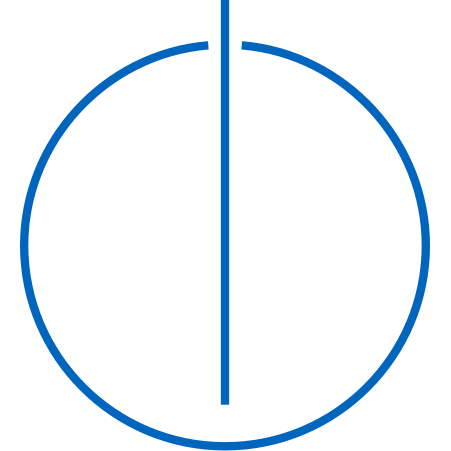
\includegraphics[height=20mm]{logos/faculty.png}
  }{}
\end{titlepage}

\frontmatter{}
\begin{titlepage}
  \centering

  \IfFileExists{logos/tum.pdf}{%
    
\includegraphics[height=20mm]{logos/tum.pdf}
  }{%
    \vspace*{20mm}
  }

  \vspace{5mm}
  {\huge\MakeUppercase{\getFaculty{}}}\\

  \vspace{5mm}
  {\large\MakeUppercase{\getUniversity{}}}\\

  \vspace{20mm}
  {\Large \getDoctype{}}

  \vspace{15mm}
  {\huge\bfseries \getTitle{} \par}

  \vspace{10mm}
  {\huge\bfseries \foreignlanguage{ngerman}{\getTitleGer{}} \par}

  \vspace{15mm}
  \begin{tabular}{l l}
    Author:          & \getAuthor{} \\
    Supervisor:      & \getSupervisor{} \\
    Advisor:         & \getAdvisor{} \\
    Submission Date: & \getSubmissionDate{} \\
  \end{tabular}

  \IfFileExists{logos/faculty.png}{%
    \vfill{}
    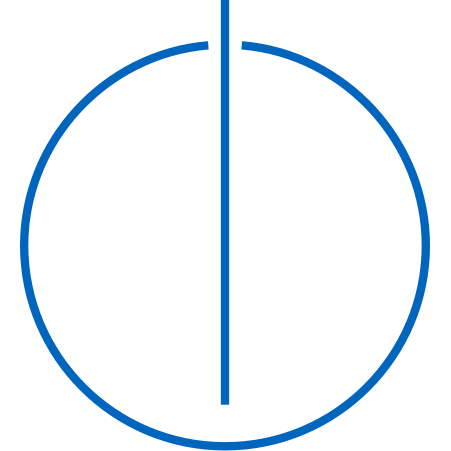
\includegraphics[height=20mm]{logos/faculty.png}
  }{}
\end{titlepage}


\thispagestyle{empty}
\vspace*{0.8\textheight}
\noindent
I confirm that this \getDoctype{} is my own work and I have documented all sources and material used.

\vspace{15mm}
\noindent
\getSubmissionLocation{}, \getSubmissionDate{} \hspace{50mm} \getAuthor{}

\cleardoublepage{}

\addcontentsline{toc}{chapter}{Acknowledgments}
\thispagestyle{empty}

\vspace*{20mm}

\begin{center}
{\usekomafont{section} Acknowledgments}
\end{center}

\vspace{10mm}

First and foremost, I would like to thank Aljo\^{s}a for his advice, guidance, and support while writing this thesis.
In particular, his vast expertise in all things concerning multi-object tracking was invaluable.
My gratitude goes towards Niko, whose SLAM proficiency immensely helped when implementing object-level Bundle Adjustment.
Last but not least, I thank my parents for their continuous support during my studies.

\cleardoublepage{}

\chapter{\abstractname}
This thesis addresses the problem of 3D \glsentrylong{mot} for RGB-based systems.
More specifically, we propose a method that performs sparse feature-based object-level \glsentrylong{ba} for accurate object track localization.
Using the 2D object detector and tracker TrackR-CNN \cite{voigtlaenderMOTSMultiObjectTracking2019}, we introduce a procedure for stereo object detections and improve TrackR-CNN's trained association ability.
We achieve superior association via a multi-stage association pipeline that combines appearance and 3D localization similarity.
Additionally, we leverage a priori knowledge of object shapes and dynamics for both association and keeping a sparse outlier-free point cloud representation of objects.

We evaluate our proposal on the KITTI \cite{geigerVisionMeetsRobotics2013} tracking dataset via the traditional CLEAR \cite{bernardinEvaluatingMultipleObject2008} and the recently introduced HOTA \cite{luitenHOTAHigherOrder2021} metrics.
However, as the official KITTI tracking benchmark only includes 2D \glsentrylong{mot} evaluation, and the extended 3D evaluation from \cite{wengBaseline3DMultiObject2019} only supports CLEAR via 3D \glsentrylong{iou}, we implement a customized
tracking ability assessment.
The evaluation introduces a normalized 3D \glsentrylong{giou} \cite{rezatofighiGeneralizedIntersectionUnion2019} detection similarity score to the official HOTA evaluation scripts.\footnote{\url{https://github.com/JonathonLuiten/TrackEval}}
We compare our performance to the LiDAR-based AB3DMOT \cite{wengBaseline3DMultiObject2019} for which 3D tracking results are readily available and demonstrate promising results, especially w.r.t. association and rigid, moving objects.
Furthermore, we show the contribution of various features of our system on an overall performance increase of 17\% for cars and 27\% for pedestrians.
The code for the proposed implementation and performance evaluation is publicly available.\footnote{\url{https://github.com/AnselmC/bamot}}


\newpage
\microtypesetup{protrusion=false}
\tableofcontents
\microtypesetup{protrusion=true}

\mainmatter{}

\chapter{Introduction \& Contribution}
\label{sec:org75ae8d0}
\section{Introduction}
\label{sec:org0ff1562}
 	Kick-started by the first autonomous vehicle race -  the 2004 DARPA Grand Challenge - the development of robotic autonomous navigation has seen substantial advancement in the previous two decades.
Research in this area encompasses a multitude of domains. 
It includes accurately localizing a robot and mapping its environment; understanding the scenery semantically and detecting and tracking other participants in the robot's surroundings is another crucial dimension - even more so in safety-critical situations such as self-driving cars. 
Path planning, trajectory prediction of detected objects, and motion control are additional essential tasks for a truly autonomous system. 
Solutions to the subproblems mentioned above exist for varying degrees of scene complexity, underlying sensor sets, and computational resources. 
However, fundamentally, autonomous navigation remains an open research problem.

Localization and map creation of the (static) environment (known as \gls{slam}) is among the most well-understood and explored dimensions of the challenge at hand. 
The main formulations based on \gls{sonar} and \gls{lidar} sensors were introduced in the 1990s and then further analyzed and developed in the previous two decades \cite{cadenaPresentFutureSimultaneous2016}.
More recently, \gls{slam} systems based on cheaper RGB-camera setups have received increasing attention and several solutions have been proposed, both for dense disparity maps \cite{engelLSDSLAMLargeScaleDirect2014} and sparse
feature-based maps \cite{engelDirectSparseOdometry2018,mur-artalORBSLAM2OpenSourceSLAM2017}. 
While these procedures work well for non-changing environments, they exhibit difficulties in highly dynamic situations where the static world assumption no longer holds.
This shortcoming has incited research that detects and then removes dynamic parts in the sensor data before running ``traditional'' \gls{slam} culminating in more robust systems \cite{yuDSSLAMSemanticVisual2018,bescosDynaSLAMTrackingMapping2018,salas-morenoSLAMSimultaneousLocalisation2013,liRGBDSLAMDynamic2017}.
This approach was substantially aided with the advent of highly performant \gls{dl} object detectors, e.g., \cite{redmonYouOnlyLook2016,heMaskRCNN2018,renFasterRCNNRealTime2017,xiangSubcategoryawareConvolutionalNeural2017}.


Detecting objects and associating detections across frames, termed \gls{mot}, is another subtask for any self-driving system (but also critical for other applications, e.g., surveillance).
While considerable research exists on tracking in 2D (i.e., in images), e.g., \cite{leal-taixeEverybodyNeedsSomebody2011,sharmaPixelsLeveragingGeometry2018,schulterDeepNetworkFlow2017,lizhangGlobalDataAssociation2008}, the requirement for 3D object localization for autonomous navigation scenarios has recently spawned numerous publications for this task:
although many depend on accurate but expensive \gls{lidar}, e.g., \cite{wengBaseline3DMultiObject2019,baserFANTrack3DMultiObject2019,yinCenterbased3DObject2021,chiuProbabilistic3DMultiObject2020}, 
there also exist implementations that only utilize image data, e.g., \cite{osepCombinedImageWorldSpace2018,luitenTrackReconstructReconstruct2020,liStereoVisionbasedSemantic2018,heneinDynamicSLAMNeed2020,barsanRobustDenseMapping2018,yangCubeSLAMMonocular3D2019,dongVisualInertialSemanticSceneRepresentation2017}.


Of these camera-based 3D multi-object trackers, \cite{liStereoVisionbasedSemantic2018,heneinDynamicSLAMNeed2020,barsanRobustDenseMapping2018,yangCubeSLAMMonocular3D2019,dongVisualInertialSemanticSceneRepresentation2017,luitenTrackReconstructReconstruct2020} combine 3D \gls{mot} and \gls{slam}. 
Such a synthesis comes naturally as both systems can benefit from each other: 
detecting objects enables more robust \gls{slam} in dynamic scenes as well as a higher-level understanding of the environment.
On the other hand, accurate robot odometry and static-map knowledge from \gls{slam} aids precise localization of objects in 3D space.


Due to the nascency of 3D \gls{mot}, most of the systems mentioned above do not evaluate their performance w.r.t. 3D \gls{mot}. 
Instead, they evaluate their 3D \gls{mod} capabilities or revert to assessing their 2D \gls{mot} ability. 
Although the work by Weng et al. \cite{wengBaseline3DMultiObject2019} proposes an extension for 3D \gls{mot} evaluation for the widely-used 2D \gls{mot} CLEAR \cite{bernardinEvaluatingMultipleObject2008} metrics, the authors use 3D \gls{iou} for calculating detection similarity.
This measure, however, does not capture 3D tracking performance well as it does not consider imprecise detections. 
While this is less of a problem for \gls{lidar} systems, detection accuracy for visual-trackers significantly decreases with camera-object distance.
Completely disregarding all of these detections does not reflect the actual tracking performance. 
Moreover, Luiten et al. \cite{luitenHOTAHigherOrder2021} recently presented an argument against current \gls{mot} metrics (including CLEAR) and proposed an alternative: \gls{hota}.

\section{Contribution}
\label{sec:org825632b}
This thesis focuses on stereo-based 3D \gls{mot} that is easily integrable with a static \gls{slam} system.
For 2D object detection, we employ TrackR-CNN \cite{voigtlaenderMOTSMultiObjectTracking2019}. 
Utilizing the tried-and-tested \gls{ba} optimization technique abundant in \gls{slam}, we implement object-level \gls{ba} based on sparse features to perform 3D object localization. 
We also exploit a priori knowledge of object shapes and dynamics for motion estimation and aggressive culling of object landmarks, thus removing outliers and keeping a sparse object representation.
We achieve robust association of detections across frames via a multi-step association pipeline: first, we compute similarity based on a novel combined appearance and 3D localization score.
For remaining detections, we corroborate the world-space motion of appearance-based association from TrackR-CNN with available 3D information. 
In a final association stage, only the Euclidean distance encodes the similarity of detections and existing tracks.

We evaluate our system's 3D \gls{mot} performance on the KITTI \cite{geigerVisionMeetsRobotics2013} tracking dataset employing a normalized \gls{giou} similarity measure and 
demonstrating results w.r.t. the CLEAR metrics as well as the newly introduced \gls{hota}.
We compare our proposal to the LiDAR-based AB3DMOT \cite{wengBaseline3DMultiObject2019} and present promising results for rigid objects in motion. 
We also investigate the impact of our system's multiple high-level features, leading to an increase of 17\% (cars) and 27\% (pedestrians) in overall performance.
Additionally, we discuss and show the capabilities and shortcomings of \gls{bamot} qualitatively.


\newpage
\chapter{Notations \& Conventions}
\label{sec:org16ce9d1}
In this work, we denote scalars as lowercase characters, e.g. \(a\), vectors as bold lowercase characters, e.g.
\(\mathbf{a}^T = \begin{pmatrix}a_x & a_y & a_z\end{pmatrix}\), and matrices as bold uppercase characters, e.g.
\(\mathbf{A} = \begin{pmatrix}a_{00} & a_{01} & a_{02} \\ a_{10} & a_{11} & a_{12} \\ a_{20} & a_{21} & a_{22}\end{pmatrix}\).
The identity matrix of dimension \(n\) is expressed as \(\mathbf{I}^n\), the 3D zero-vector as \(\mathbf{0}\), and the n-dimensional zero matrix (all entries zero) as \(\mathbf{0}^n\). 
\(|\mathbf{a}| = \sqrt{a_x^2 + a_y^2 + a_z^2}\) denotes the length of a vector \(\mathbf{a}\). 
Additionally, \(\mathbf{A}^T\) (\(\mathbf{a}^T\)) is the transpose of a matrix (vector) \(\mathbf{A}\) (\(\mathbf{a}\)) and similarly the inverse of a matrix \(\mathbf{A}\) is \(\mathbf{A}^{-1}\).
A matrix's trace (i.e., the sum of the elements of its main diagonal) is written as \(\text{tr}(\mathbf{A})\).
The cross-product of two vectors is denoted by ``\(\times\)'' and the dot product by ``\(\cdot\)'':
\(\mathbf{a} \times \mathbf{b} = \begin{pmatrix}a_yb_z - a_zb_y \\ a_zb_x - a_xb_z \\ a_xb_y - a_yb_x\end{pmatrix}\) and \(\mathbf{a} \cdot \mathbf{b} = \mathbf{a}^T\mathbf{b}\), respectively. 
Furthermore, a bold uppercase character with indices in the following manner express transformations (see \cref{theoretical-background}) from coordinate system \(Y\) to coordinate system \(X\): \({}^X_Y\mathbf{T}\). If a time component \(t\) is involved, this expression is enhanced: \({}^X_Y\mathbf{T}_t\).
We denote a point/vector \(\mathbf{p}\) given in a specific coordinate system \(X\) as \({}^X\mathbf{p}\).
Further, non-recurring additions to this notation are explained as needed.
All coordinate systems are right-handed (see \cref{fig:right-vs-left-cosy}). 

\begin{figure}[htbp]
\centering
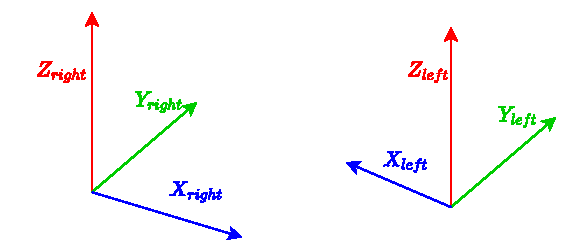
\includegraphics[width=0.5\textwidth]{figures/right-vs-left-cosy.pdf}
\caption{\label{fig:right-vs-left-cosy}Two possible ways to represent coordinate systems. In SLAM one commonly uses the right-handed coordinate system which we adopt for this thesis.}
\end{figure}

\chapter{Theoretical Background \label{theoretical-background}}
\label{sec:org87931b0}
\section{Multiple Object Detection and Tracking \label{modat}}
\label{sec:orgd7d93ac}
   Detecting objects in the sensory output of imaging systems (e.g., RGB images or \gls{lidar} scans) has been a cornerstone to \gls{cv} research since its advent in the mid-sixties of the 20th century \cite{papert1966summer}. It is fundamental to most robotics-related applications today (e.g., surveillance systems or, possibly less dystopian, autonomous driving). Typically, an object detection consists either of a bounding box
 (2D for RGB images, 3D for RGB-D or LiDAR) around said object or, in more precise methods, of pixel- or voxel-wise (for 2D and 3D input, respectively) detections. 
If an object detector can detect more than one type of object, each detection is usually accompanied by a class prediction (e.g., cat, dog, or car). Usually, a detector should also be capable of detecting more than
one object in its input domain. 
Furthermore, frequently merely detecting objects does not suffice: being able to associate detections across multiple input frames (e.g., a video stream) is paramount to understanding a dynamic environment.
This linking of single detections over time is known as object tracking.

\subsection{Classical object detection}
\label{sec:orgd57420f}
    Some of the earliest research on object detection relates to finding humans (or their faces) in images such as the ``Eigenface'' approach introduced in \cite{sirovichLowdimensionalProcedureCharacterization1987a} and based on \gls{pca}, 
a \gls{hog} method patented in \cite{mcconnellMethodApparatusPattern}, or a ML-based system proposed in \cite{violaRobustRealtimeFace2004} known as the Viola-Jones detector. 
All of these approaches extract lower-level image features (such as edges, points, or statistical attributes) and then employ varying techniques (often ML-based) 
to recognize objects based on specific features or clusters thereof.
\cref{fig:classical-object-detection} exemplifies representations of feature spaces for some of these procedures.
Although these techniques work sufficiently well in specific scenarios (e.g., face detection based on Viola-Jones), they 
are limited to a single (or very few) object classes, output imprecise bounding boxes for detections, and often require extensive feature-engineering, 
i.e., how and which low-level characteristics are extracted from the input and fed to a machine-learning algorithm for classification.

\begin{figure}[htbp]
\centering
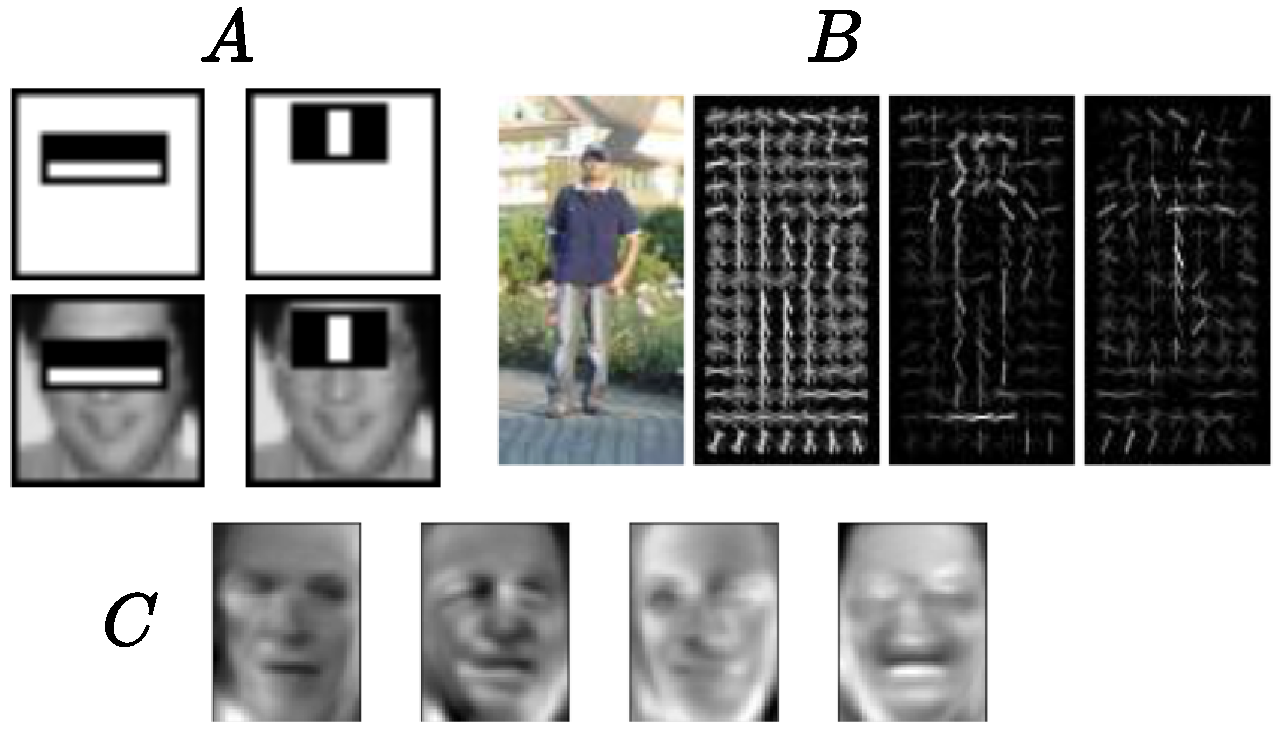
\includegraphics[width=0.5\textwidth]{figures/classical-object-detection.pdf}
\caption{\label{fig:classical-object-detection}\emph{Top Left (A)}: Two example filters/features learned by a Viola-Jones detector for face detection \cite{violaRobustRealtimeFace2004}. \emph{Top Right (B, from left to right)}: An example input image followed by its Histogram-of-Oriented-Gradients representation and two results of learned output weighting of the HOGs for people detection \cite{dalalHistogramsOrientedGradients2005}. \emph{Bottom (C)}: Various examples of eigenfaces used for face detection and recognition (taken from \url{https://scikit-learn.org/stable/auto\_examples/applications/plot\_face\_recognition.html}).}
\end{figure}

\subsection{Deep object detection}
\label{sec:orgc65b510}
    Another early object detection task was recognizing letters, a technique known as \gls{ocr} \cite{schantzHistoryOCROptical1982}.
These feature-engineering heavy systems were revolutionized by the first automatic gradient-based image-filter \gls{dnn} \cite{lecunGradientbasedLearningApplied1998}, introducing a class of \glspl{nn} known today as \glspl{cnn}.
\gls{cnn} are multi-layered \gls{nn} that utilize learned shift-invariant filters to understand locally-correlated input data (e.g. images) for a plethora of tasks including, first and foremost, 
object detection \cite{krizhevskyImageNetClassificationDeep2017}, \cite{renFasterRCNNRealTime2017}, \cite{redmonYouOnlyLook2016}).
Detailed overviews, explanations and discussions on \gls{dl} and, more specifically, \gls{cnn}, can be found in 
\cite{bishopPatternRecognitionMachine2006}, \cite{heatonIanGoodfellowYoshua2018}, and \cite{GuideConvolutionalNeural2017} for example.
The above-cited object detection networks produce bounding boxes and their respective class predictions. 
However, pixel-level object detection networks such as \cite{heMaskRCNN2018} compute so-called segmentation masks and class predictions per mask. \cref{fig:mask-vs-bbox} shows a comparison
of bounding box vs. segmentation mask detections.

\begin{figure}[htbp]
\centering
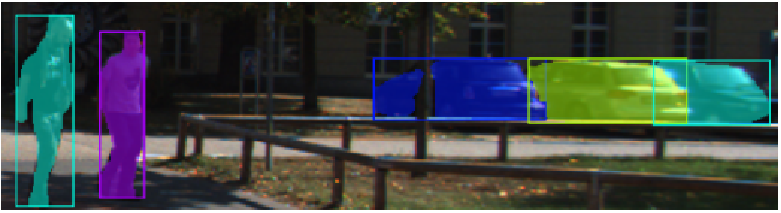
\includegraphics[width=0.75\textwidth]{figures/mask-vs-bbox.pdf}
\caption{\label{fig:mask-vs-bbox}Rectangular bounding boxes are a poor fit for capturing a person's geometry - segmentation masks do this far better. Additionally, segmentation masks are also superior when objects overlap.}
\end{figure}

This pixel-wise precision of object detections is instrumental and even necessary when objects occlude each other or do not fill-out a rectangle very well (as is mostly the case).
3D object detectors that work on \gls{lidar} or RGB-D data as input have also been proposed \cite{kuJoint3DProposal2018}, \cite{wengMonocular3DObject2019a}, \cite{qiFrustumPointNets3D2018}, \cite{shiPointRCNN3DObject2019a}. 
The standard way to describe a 3D object detection is by the seven \glspl{dof} \gls{oobb}. This \gls{oobb} consists of a Euclidean location (\(x\), \(y\), \(z\)), the object's dimensions (height, width, length), and its rotation around gravity (more commonly referred to as its yaw). Note that much like 2D bounding boxes in the image domain, this type of description does not necessarily describe an object well, i.e., it assumes
that objects travel along a fixed plane, only rotate around a single axis, and nicely fill out a rectangular box.


\subsection{Object Tracking \label{object-tracking}}
\label{sec:orga483366}
    As previously mentioned, detecting objects is frequently accompanied by tracking object instances over time. 
There exist two fundamental approaches to tracking: offline and online tracking.
Offline tracking tries to associate detections after-the-fact: given an entire sequence of \(i\) images and \(n_j\) detections for a given image, these methods try to find the globally optimal tracks.
One possibility to solving such global optimization is to pose the tracking problem as a \gls{mcfp} \cite{ahujaNetworkFlowsTheory1993} where detections constitute nodes and the flow along a collection of nodes makes up a track \cite{lizhangGlobalDataAssociation2008,schulterDeepNetworkFlow2017,leal-taixeEverybodyNeedsSomebody2011}.

On the other hand, online tracking associates detections in a streaming fashion, i.e., by processing images and the detections in these images sequentially. Hence at every step, detections need to be matched with
existing object tracks; if the system doesn't match a given detection, it creates a new track. 
One generally formulates the matching problem as a bipartite graph problem where one collection of nodes are the detections \(U_{detections}\) 
and the other are the existing object tracks \(V_{tracks}\) (see \cref{fig:bipartite-graph}). 

\begin{figure}[htbp]
\centering
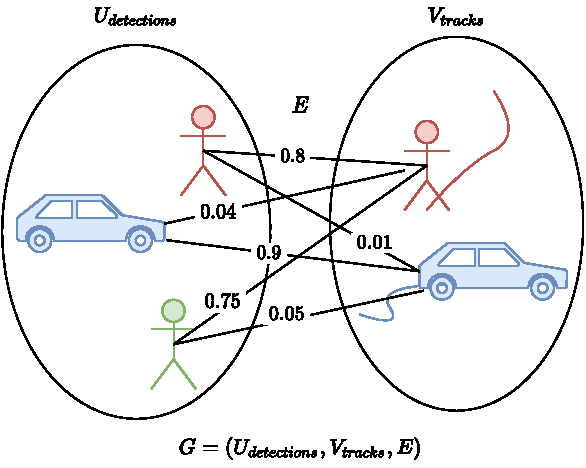
\includegraphics[width=0.5\textwidth]{figures/bipartite-graph.pdf}
\caption{\label{fig:bipartite-graph}The association problem stated as a bipartite graph where one set of nodes are object detections, the other set are object tracks, and the weights of the edges connecting nodes between these two sets are the similarities (or dissimilarities) between each track-detection combination.}
\end{figure}

The edges \(E\) between nodes \(i \in U_{detections}\) and \(j \in V_{tracks}\) of these two sets are weighted by some similarity score \(S(i, j)\) and the optimization goal is to maximize the total similarity by matching all nodes from the respective sets.

\subsubsection{Hungarian Algorithm}
\label{sec:org0b5702f}
    The Hungarian Algorithm \cite{kuhnHungarianMethodAssignment1955} solves the optimization problem of maximizing the sum of the weights of a matching \(M\) between \(U_{detections}\) and \(V_{tracks}\) for the graph \(G =(U_{detections}, V_{tracks}, E)\).
If minimizing similarity is the goal, one can trivially accomplish this by multipliying similarities by \(-1\) and then maximizing the total inverse similarity.

The algorithm introduces the notion of labels for nodes (denoted by \(l(.)\)) where \(l(i) + l(j) \leq w(i, j)\) and from this the equality graph \(G_{l} = (U_{detections}, V_{tracks}, E_l)\) where \(E_l\) only includes edges whose weights 
are equal to the sum of the labels of the nodes, i.e., \(w_l(i, j) = l(i) + l(j)\).
The central theorem of the Hungarian Algorithm is that any \emph{perfect} matching \(M_l\) in this equality graph maximizes the edge weights in the original graph, and hence is an optimal matching \(M\). 
A perfect matching is a matching where all nodes from \(U_{detections}\) are matched to a single node in \(V_{tracks}\) and vice versa, i.e., a 1-to-1 mapping. 
Of course, the number of elements of the node sets may be unequal. Introducing ``dummy'' elements to the smaller set with similarity scores of zero to all other elements in the other set can resolve this discrepancy.
To initialize the algorithm, the labels for nodes in \(U_{detections}\) are set to the maximum weight of outgoing edges, whereas the labels for nodes in \(V_{tracks}\) start at 0. 
This labeling trivially fulfills \(l(i) + l(j) \geq w(i, j)\) and the algorithm now constructs \(E_l\) by adding edges for which \(l(i) + l(j) = w(i, j)\) holds.
Additionally, \(M_l\) initializes to the empty set.

The algorithm now improves \(M_l\) via two procedures: augmenting paths and improving labels.
First, the algorithm searches for an augmented path, e.g., via \gls{bfs}. 
An augmented path is a path that starts at a node \(u \in U_{detections}\) and ends at a node \(v \in V_{tracks}\) both of which are not connected to an edge in \(M_l\). 
Furthermore, the edges in \(E_l\) connecting these nodes must alternately already belong to \(M_l\) and not be part of it. The nodes visited by a path in \(V_{tracks}\) are cached as \(S \subset V_{tracks}\) and likewise
the nodes visited in \(U_{detections}\) are tracked in \(T \subset U_{detections}\).

If an augmented path is found, the procedure adds the edges of the path that were not in \(M_l\) to \(M_l\). It also removes the edges that were previously in \(M_l\) from the matching.
On the other hand, if an augmented path is not found, the algorithm optimizes the labels \(l(.)\) in such a way that existing edges of \(M_l\) remain in \(E_l\), i.e., \(l(i) + l(j) = w(i, j)\).
It then adds new edges to \(E_l\) that fulfill this property.
The algorithm avhieves this by computing a \(\delta\) based on visited nodes \(s \in S\) and unvisited nodes \(y \in U_{detections} \setminus T\) as follows:
\begin{equation}
\delta = \min_{s, y} \{l(s) + l(y) - w(s, y)\}
\end{equation}

From this one constructs a new labeling:

\begin{equation}
l'(n) = 
\begin{cases}
l(n) - \delta ~\text{iff}~ n \in S \\
l(n) + \delta ~\text{iff}~ n \in T \\
l(n) ~\text{else}~
\end{cases}
\end{equation}

This two-step process of finding augmented paths and improving the node labelling repeats until all nodes of both sets are matched.

In scenarios such as object tracking, one doesn't require a one-to-one matching. In fact in many situations such a mapping is not desirable, e.g. when an old object leaves the view and a new object enters it.
Thus, a similarity threshold can help: a match between two nodes \(u \in U_{detections}, v \in V_{tracks}\) is only valid if the similarity scores between them are greater than an application-specific threshold, i.e., \(S(u, v) \geq \alpha\). 
An alternative implementation for solving the Hungarian Algorithm uses adjacency matrices.

Some examples of online 2D trackers include \cite{voigtlaenderMOTSMultiObjectTracking2019,bewleySimpleOnlineRealtime2016};
instances of object trackers operating in 3D space \(\mathbb{E}^3\) (i.e., via \gls{oobb}) are \cite{wengBaseline3DMultiObject2019,osepCombinedImageWorldSpace2018}.


\section{3D Geometry \label{3d-geometry}}
\label{sec:org85187ac}
\subsection{Transformations in 3D space \label{transformations-3d}}
\label{sec:org8db448f}
   An important part of any robotics-related application is describing rotations and translations of rigid bodies in 3D.
These transformations must preserve the following properties \cite{bottemaTheoreticalKinematics1990} w.r.t. two vectors or points \(\mathbf{a}, \mathbf{b} \in \mathbb{R}^3\):

\begin{enumerate}
\item their distance to each other, i.e., \(|\mathbf{a} - \mathbf{b}| = |q(\mathbf{a}) - q(\mathbf{b})|\)
\item the orientation between them, i.e., \(q(\mathbf{a} \times \mathbf{a}) = q(\mathbf{a}) \times q(\mathbf{b})\)
\end{enumerate}

Given a fixed world coordinate frame, a three \glspl{dof} translation can be trivially expressed by a 3D vector \(\mathbf{t}^T=\begin{pmatrix}t_x & t_y & t_z\end{pmatrix}\).

A rotation in 3D Euclidean space also has three \glspl{dof} but has multiple representations \cite{mccarthyIntroductionTheoreticalKinematics1990}:
\begin{enumerate}
\item as a unit-length rotation axis \(\mathbf{u}\) and an angle \(\theta\) around that axis (axis-angle representation)
\item as a unit quaternion \(\mathbf{q} = q_r + q_i\mathbf{i} + q_j\mathbf{j} + q_k\mathbf{k}~\text{with}~|\mathbf{q}|=1~\text{and}~q_i\in\mathbb{R}\) where \(i, j, k\) are imaginary and special mathematical properties apply
\item as \(\mathbf{R}\), a \(3\times3\) orthogonal (i.e., \(\mathbf{R}\mathbf{R}^T=\mathbf{I}\) \cite{murrayMathematicalIntroductionRobotic1994}) rotation matrix with \(\text{det}(\mathbf{R}) = 1\) for right-handed systems (and \(\text{det}(\mathbf{R}) = -1\) for left-handed systems)
\item as a combination of three successively applied rotations around three orthogonal axes (Euler angles).
\end{enumerate}

In the following, we will deal with rotations in their axis-angle representation when expressing incremental rotations. Otherwise, we will use their matrix representations as this enables computationally efficient matrix-vector multiplication.
Computing the corresponding rotation matrix from a rotation axis \(\mathbf{u}\) and an angle \(\theta\) can be achieved with Rodrigues' formula \cite{murrayMathematicalIntroductionRobotic1994}:

\begin{equation}
\label{eq:rodrigues}
\mathbf{R} = \mathbf{I} + (1-\cos(\theta))\mathbf{u}^\wedge\mathbf{u}^\wedge + \sin(\theta)\mathbf{u}^\wedge
\end{equation}

\(\mathbf{u}^{\wedge}\) in \cref{eq:rodrigues} is the skew-symmetric matrix representation of a vector:
\begin{equation}
\mathbf{u}^\wedge = \begin{pmatrix}0 & -u_z & u_y \\ u_z & 0 & -u_x \\ -u_y & u_x & 0 \end{pmatrix}
\end{equation}
This skew-symmetric representation is useful as it linearizes the cross-product between two vectors:
\begin{equation}
\mathbf{a} \times \mathbf{b} = \mathbf{a}^\wedge \mathbf{b}
\end{equation}
The property giving this representation its name is skew-symmetry: \((\mathbf{u}^\wedge)^T = -\mathbf{u}^\wedge\).

Inversely, one can calculate the angle and rotation axis from a rotation matrix as follows:

\begin{enumerate}
\item compute the angle: \(\theta = \arccos(\frac{\text{tr}(\mathbf{R})-1}{2})\)
\item solve the system of equations given by the following relation: \(\mathbf{R}\mathbf{u} = \mathbf{u}\)
\end{enumerate}

The combination of rotation and translation is also a rigid body transformation \(\mathbf{T}\) and describes arbitrary transformations in 3D Euclidean space \(\mathbb{E}^3\).
Such a transformation can be expressed as the rotation of a vector/point followed by its translation: \(\tilde{\mathbf{a}} = \mathbf{R}\mathbf{a} + \mathbf{t}\).
However, ideally, a transformation should be expressed by a single operation.

\cref{fig:rigid-transformation} gives an example of a rigid body transformation from an initial frame A to the final frame B.
\begin{figure}[htbp]
\centering
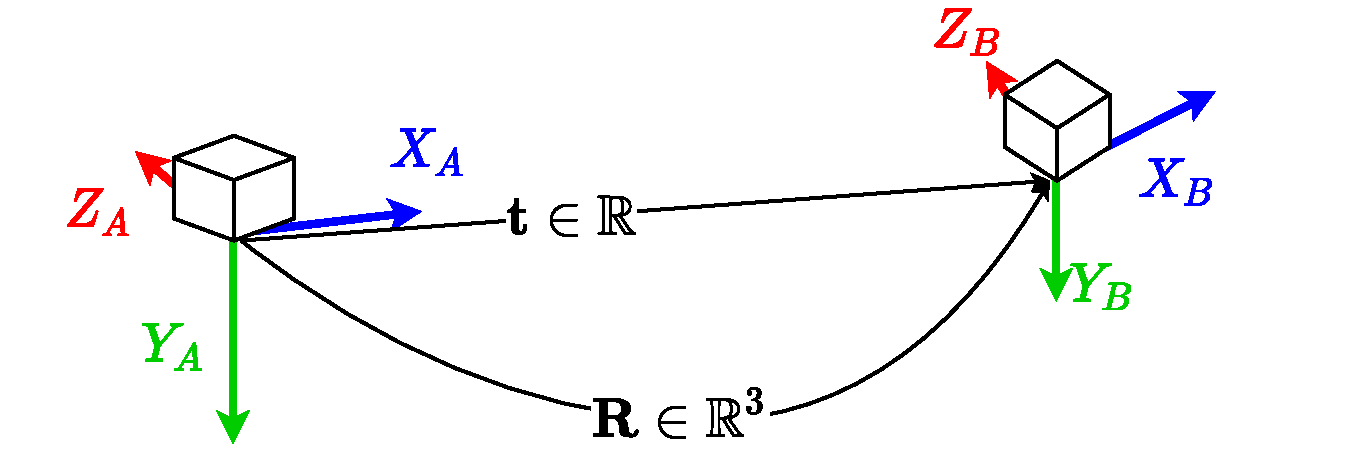
\includegraphics[width=.9\linewidth]{figures/rigid-transformation.pdf}
\caption{\label{fig:rigid-transformation}A rigid body undergoes a transformation in Euclidean space \(\mathbb{E}^3\) from frame A to frame B.}
\end{figure}

\subsection{Homogeneous Coordinates \label{homogeneous-coordinates}}
\label{sec:org312b44c}
    Homogeneous coordinates are a standard tool for transforming points/vectors in a linearized fashion via matrix multiplication \cite{murrayMathematicalIntroductionRobotic1994}. 
Combining the rotational and translational part of a Euclidean transformation into a single 4-by-4 matrix \(\mathbf{T}=\begin{bmatrix} \mathbf{R}  & \mathbf{t} \\ \mathbf{0}^T & 1 \end{bmatrix}\) and 
using the homogeneous representation of Euclidean vectors allows for such computationally desired multiplication (see \cref{eq:homogeneous}) forgoing the need of rotating a vector first and then translating it as described
previously.
In homogeneous coordinates a scaling factor \(w\) is added as the fourth dimension s.t. the vector \(\mathbf{a}^T = \begin{pmatrix}x & y & z\end{pmatrix}\) is represented as \(\mathbf{\tilde{a}}^T = \begin{pmatrix}x\cdot w & y\cdot w & z \cdot w & w\end{pmatrix}\). 
To transform a homogeneous coordinate to Euclidean space, one merely divides the homogeneous vector by \(w\) and discards the fourth dimension (which equals one after division). 
Inversely, to transform a Euclidean vector to its homogeneous counterpart, one can simply multiply all elements by a scaling factor \(w \neq 0\) and add this factor as the fourth dimension to the vector. 
For simplicity, one usually chooses \(w\) to be one. Observe that this results in the fact that homogeneous vectors have infinite representations, whereas their Euclidean complements are unique.
\begin{equation}
\label{eq:homogeneous}
\begin{bmatrix} \mathbf{R}  & \mathbf{t} \\ \mathbf{0}^T & 1 \end{bmatrix}\begin{pmatrix}\mathbf{v} \\ 1 \end{pmatrix}
= \begin{pmatrix}\mathbf{R}\mathbf{v} + \mathbf{t} \\1\end{pmatrix}
\end{equation}

\subsection{Groups \label{groups}}
\label{sec:orgc365e94}
    Group theory is the study of so-called mathematical groups and plays a vital role in algebra, the natural sciences, and engineering. 
A group is the combination of some set \(\mathbf{G}\) and a binary operator \(\cdot\) for which the following four axioms must hold \cite{murrayMathematicalIntroductionRobotic1994}: 
\begin{itemize}
\item \emph{Closure}: combining two elements \(a, b \in \mathbf{G}\) with the binary operator produces another element which is part of the group, i.e., \(a\cdot b=c\in \mathbf{G}\)
\item \emph{Associativity}: \(\forall a, b, c \in \mathbf{G}\) it must hold that \((a\cdot b) \cdot c = a \cdot (b\cdot c)\)
\item \emph{Identity}: there must exist an identity element \(e \in \mathbf{G}\) s.t. \(a \cdot e = a ~\forall a \in \mathbf{G}\)
\item \emph{Invertibility}: for every element \(a\) there must be a (unique) inverse element \(a^{-1} \in \mathbf{G}\) such that \(a \cdot a^{-1} = e\).
\end{itemize}

A basic example of a group is the set of integers \(\mathbb{Z}\) under addition, and typical examples
of non-Groups are the set of integers under multiplication or the set of natural numbers \(\mathbb{N}\)
combined with addition \cite{langAlgebra2002}.

\subsubsection{Lie Groups and Lie Algebras \label{lie-groups}}
\label{sec:org04d1374}
    So-called Lie groups are a subset of groups. These types of groups have the additional unique property that they
locally (i.e., close to an element's identity) approximate Euclidean space and, hence, allow one to perform Euclidean calculus such as differentiation.
Differentiation implicitly then allows parameterizing an element by the variable being differentiated by, e.g., time.

This informal definition is more correctly described as Lie groups exhibiting the attribute of being a smoothly
differentiable manifold, or topological space \cite{adamsLecturesExceptionalLie1996}.

One can investigate this local resemblance to Euclidean space via its tangent space.
The tangent space close to the identity of a Lie group is called the Lie algebra \(\mathfrak{g}\). 
Its vector space  \(\mathbb{V}\) (i.e., the space making up its elements) over some field \(\mathbb{F}\) (i.e., the field where its elements are defined) 
and a binary operator, its Lie bracket, \([,]\), characterize a Lie algebra.

This Lie bracket is an alternating bilinear mapping that satisfies the Jacoby identity given by \cref{eq:jacobi-id} \cite{hallLieGroupsLie2015}. 

\begin{equation}
\label{eq:jacobi-id}
\begin{split}
& \forall \mathbf{X}, \mathbf{Y}, \mathbf{Z} \in  \mathbb{V} , \\ 
& [\mathbf{X}, [\mathbf{Y}, \mathbf{Z}]] + [\mathbf{Z}, [\mathbf{X}, \mathbf{Y}]] + [\mathbf{Y}, [\mathbf{Z}, \mathbf{X}]] = \mathbf{0}
\end{split}
\end{equation}

\newpage
An alternating bilinear mapping is defined as a binary operator for which
the following assumptions must hold \cite{hallLieGroupsLie2015}:

\begin{itemize}
\item \emph{Closure}: operations are closed under composition, i.e.,  \(\forall \mathbf{X}, \mathbf{Y} \in \mathbb{V} \rightarrow [\mathbf{X}, \mathbf{Y}] \in \mathbb{V}\).
\item \emph{Bilinearity}: the Lie algebra must satisfy the bilinear form as given in \cref{eq:bilinear-form}
\item \emph{Alternativity}: application of the operator on the element and itself must result in the origin vector, i.e., \(\forall \mathbf{X} \in \mathbb{V} \rightarrow [\mathbf{X}, \mathbf{X}] = \mathbf{0}\).
\end{itemize}

\begin{equation}
\label{eq:bilinear-form}
\begin{split}
& \forall \mathbf{X}, \mathbf{Y}, \mathbf{Z} \in  \mathbb{V} \wedge u, w \in \mathbb{F}  \\
& [u\mathbf{X} + b\mathbf{Y}, \mathbf{Z}] = \\
& u[\mathbf{X}, \mathbf{Z}] + w[\mathbf{Y}, \mathbf{Z}] \\
& \wedge \\
& [\mathbf{Z}, u\mathbf{X} + w\mathbf{Y}] = \\ 
& = u[\mathbf{Z}, \mathbf{X}] + w[\mathbf{Z}, \mathbf{Y}]
\end{split}
\end{equation}
These axioms of an alternating bilinear map can be more
succinctly denoted with the syntax given in \cref{eq:alt-bi-map}.

\begin{equation}
\label{eq:alt-bi-map}
\mathfrak{g} \times \mathfrak{g} \rightarrow \mathfrak{g}, (\mathbf{X}, \mathbf{Y}) \mapsto [\mathbf{X}, \mathbf{Y}]
\end{equation} 

A more rigorous and in-depth definition can be found in \cite{hallLieGroupsLie2015} or \cite{erdmannIntroductionLieAlgebras2006}.

\subsection{The Special Orthogonal Group SO(3) and its Lie Algebra \(\mathfrak{so}(3)\) \label{so3}}
\label{sec:org1b22466}
    N-dimensional rotations, or more specifically for the case of 3D space, three-dimensional rotations form a
Lie group called the Special Orthogonal Group SO(n) and SO(3), respectively. 
The Special Orthogonal Group are all elements of \(n \times n\) matrices with orthogonal columns and (in right-handed coordinate systems) a determinant of 1 (as previously alluded to in \cref{transformations-3d}).
\cref{eq:son-group} gives the formal definition.

\begin{equation}
\label{eq:son-group}
SO(n)=\{\mathbf{R} \in  \mathbb{R}^{n\times n}|\mathbf{R}\mathbf{R^T} = \mathbf{I^n}, \text{det}(\mathbf{R}) = 1\} 
\end{equation}

The proofs of the three axioms for (Lie) groups as described in \cref{lie-groups} are outside of this work's scope but are demonstrated in \cite{murrayMathematicalIntroductionRobotic1994} or \cite{hallLieGroupsLie2015}.

We now consider the more specific Special Orthogonal Group in three dimensions SO(3).
Rotational matrices have the computationally desirable property that they linearize rotating a vector. Linear operations are very efficient on modern CPUs.
However, a ``problem'' with rotation matrices is that there exists no notion of an infinitesimal rotation matrix. Hence, they can't be parametrized by time - which is crucial in any dynamic (e.g., robotics) application.
As mentioned earlier, the combination of a unit-length rotation axis \(\mathbf{u}\) and an angle around that axis \(\theta\) can also describe a rotation.
In this representations there exist infinitesimal rotations, i.e., when \(d\theta \rightarrow 0\).
Thus, we would like a transformation from rotation matrices to their corresponding angle-axis representation and vice versa.
To get there, assume that we rotate some point \(\mathbf{p}\) around an axis \(\mathbf{u}\) at constant unit velocity:
\begin{equation}
\mathbf{\dot{p}}(t) = \mathbf{u} \times \mathbf{p}(t) = \mathbf{u}^\wedge \mathbf{p}(t)
\end{equation}
This gives us the velocity at point \(\mathbf{p}\) at time \(t_0=0\) in the form of a time-invariant \gls{ode} whose solution is 
\begin{equation}
\mathbf{p}(t) = e^{\mathbf{u}^{\wedge}t}\mathbf{p}(t_0)
\end{equation}
Here \(e^\mathbf{A}\) is the matrix exponential given by the Taylor's Series \(e^\mathbf{A} = \mathbf{I} + \mathbf{A} + \frac{\mathbf{A}^2}{2!} + \frac{\mathbf{A}^3}{3!} \dots\).
Hence, rotating a point for \(\theta\) units of time produces a functional relationship between the resulting net rotation and the angle and axis of this rotation:
\(\mathbf{R}(\theta, \mathbf{u}) = e^{\mathbf{u}^{\wedge}\theta} = e^{\boldsymbol{\phi}}\)
The skew-symmetric elements \(\boldsymbol{\phi}\) representing an angle-axis combination make up the Lie algebra \(\mathfrak{so}(3)\) to the Lie group \(SO(3)\), 
formally defined in \cref{eq:so3} \cite{murrayMathematicalIntroductionRobotic1994}.

\begin{equation}
\label{eq:so3}
\mathfrak{so}(3) =\{\boldsymbol{\phi} \in \mathbb{R}^{3\times3} | \boldsymbol{\phi} = \phi^\wedge, \phi \in \mathbb{R}^3 \}
\end{equation}

The associated Lie bracket is \([\boldsymbol{\phi}_1, \boldsymbol{\phi}_2] = \boldsymbol{\phi}_1\boldsymbol{\phi}_2 - \boldsymbol{\phi}_2\boldsymbol{\phi}_1\).
The derived functional relationship between elements of \(\mathfrak{so}(3)\) and those in \(SO(3)\) is called the exponential map and can be simplified as follows: 

\begin{equation}
\label{so3-expmap}
\mathbf{R}(\boldsymbol{\phi}) = \mathbf{R}(\theta \mathbf{u}^\wedge) = e^{\theta \mathbf{u}^\wedge} = \mathbf{I} + (1-\cos(\theta))\mathbf{u}^\wedge\mathbf{u}^\wedge + \sin(\theta)\mathbf{u}^\wedge
\end{equation}

\cref{so3-expmap} is precisely the Rodrigues formula \ref{eq:rodrigues} mentioned in \cref{transformations-3d}.
The inverse operation, mapping from rotation matrices to the corresponding axis-angle representation \(\boldsymbol{\phi}\), is the logarithmic map:
\(\boldsymbol{\phi}(\mathbf{R}) = \ln(\mathbf{R})\)
\cref{eq:so3-log} shows how the angle \(\theta\) and axis \(\mathbf{u}\) can be derived from a rotation matrix \(\mathbf{R}\). \cite{murrayMathematicalIntroductionRobotic1994} describes the derivation in full detail.

\begin{equation}
\label{eq:so3-log}
\begin{split}
& \theta = \arccos(\frac{\text{tr}(\mathbf{R})-1}{2}) \\
& \mathbf{u} = \frac{1}{2\sin(\theta)} \begin{bmatrix}r_{32} - r_{23} \\ r_{13} - r_{31} \\ r_{21} - r_{12}\end{bmatrix}
\end{split}
\end{equation}

\subsection{The Special Euclidean Group SE(3) and its Lie Algebra \(\mathfrak{se}(3)\) \label{se3}}
\label{sec:org0584930}
    The Special Euclidean Group SE(3) is informally an extension of SO(3) that covers arbitrary rigid-body transformations, i.e., the combination of a rotation and a translation.
As already noted, 4-by-4 matrices constructed from a rotation matrix \(\mathbf{R}\) and a translational vector \(\mathbf{t}\) also represent such transformations.
The set of these transformations forms the Special Euclidean Group:
\begin{equation}
SE(3) = \{\mathbf{T} \in \mathbb{R}^{4 \times 4} | \mathbf{T}=\begin{bmatrix} \mathbf{R}  & \mathbf{t} \\ \mathbf{0}^T & 1 \end{bmatrix}, \mathbf{R} \in SO(3), \mathbf{t} \in \mathbb{R}^3\}
\end{equation}
As for SO(3), there is an equivalent generalization to \(n\) dimensions.

Similarly to SO(3), we need a different representation that resembles Euclidean space, enabling differentiation. Unsurprisingly, this space, the Lie algebra \(\mathfrak{se}(3)\), consists of six-dimensional vectors,
where three dimensions represent the translational component \(\boldsymbol{\rho}\). The other three represent the rotational element \(\boldsymbol{\phi} \in \mathfrak{so}(3)\).
Utilizing the \(\vee\) (vee) operator, which transforms a skew-symmetric matrix to its vector representation, \cref{eq:se-3} formally defines this algebra.

\begin{equation}
\label{eq:se-3}
\mathfrak{se}(3) = \{\xi^\wedge \in \mathbb{R}^{4 \times 4} | \xi = \begin{pmatrix}\boldsymbol{\rho} \\ \boldsymbol{\phi}^\vee\end{pmatrix}, \boldsymbol{\rho} \in \mathbb{R}^3, \boldsymbol{\phi} \in \mathfrak{so}(3)\}
\end{equation}

Analogously to SO(3) and following the example of \cite{murrayMathematicalIntroductionRobotic1994}, to get to a mapping between SE(3) and \(\mathfrak{se}(3)\) consider rotating a point \(\mathbf{p}\) 
around an axis \(\mathbf{u}\) and translating the point by \(\mathbf{t}\).
We can describe the velocity of said point like so:
\begin{equation}
 \dot{\mathbf{p}}(t) = \mathbf{u} \times (\mathbf{p}(t) - \mathbf{t}) = \mathbf{u}^\wedge \mathbf{p}(t) - \mathbf{u}^\wedge \mathbf{t}.
\end{equation}
We now reformulate this using homogeneous coordinates and matrix-vector multiplication as 
\begin{equation}
\begin{pmatrix}\dot{\mathbf{p}} \\ 0\end{pmatrix} = \begin{bmatrix}\mathbf{u}^\wedge & -\mathbf{u}^\wedge \mathbf{t} \\ \mathbf{0}^T & \mathbf{0} \end{bmatrix}\mathbf{p}(t) = \begin{bmatrix}\mathbf{u}^\wedge & \boldsymbol{\rho} \\ \mathbf{0}^T & \mathbf{0} \end{bmatrix}\mathbf{p}(t) = \boldsymbol{\xi}^\wedge \mathbf{p}(t).
\end{equation}
Again, we arrive at a differential equation whose solution is the exponential map: \(\mathbf{p}(t) = e^{\boldsymbol{\xi^\wedge} t}\mathbf{p}(0)\). We then perform a rotation for \(\theta\) units of time \(t\) to arrive at 
\begin{equation}
\mathbf{T}(\theta, \mathbf{u}, \mathbf{t}) = e^{\boldsymbol{\xi}^\wedge\theta}.
\end{equation}
\(\boldsymbol{\xi}^\wedge\) is also known as the twist-parametrization of a rigid-body transformation.

\cref{eq:se3-expmap} gives the closed-form solution \cite{murrayMathematicalIntroductionRobotic1994}.

\begin{equation}
\label{eq:se3-expmap}
\mathbf{T}(\theta, \mathbf{u}, \mathbf{t}) = e^{\boldsymbol{\xi}^\wedge\theta}
= \begin{pmatrix} e^{\mathbf{u}^\wedge \theta} & (\mathbf{I} + \frac{1-\cos(\theta)}{\theta}\mathbf{u}^\wedge + \frac{\theta - \sin(\theta)}{\theta}\mathbf{u}^\wedge \mathbf{u}^\wedge )\boldsymbol{\rho} \\ \mathbf{0}^T & 1\end{pmatrix}
= \begin{pmatrix} e^{\mathbf{u}^\wedge \theta} & \mathbf{J}\boldsymbol{\rho} \\ \mathbf{0}^T & 1\end{pmatrix}.
\end{equation}

Computation of the angle \(\theta\) and rotation axis \(\mathbf{u}\) from \(\mathbf{R}\) is equivalent to the log map of SO(3) (see \cref{eq:so3-log}). \cref{eq:se3-logmap} describes the recovery of the 
translational component \(\boldsymbol{\rho}\) from the translation \(\mathbf{t}\) and the previously computed angle and rotation axis.

\begin{equation}
\label{eq:se3-logmap}
\boldsymbol{\rho}(\mathbf{t}, \theta, \mathbf{u}) = \mathbf{J}^{-1}\mathbf{t} = (\mathbf{I} - \frac{\theta}{2}\mathbf{u}^\wedge + (1 - \frac{\theta(1+\cos(\theta))}{2\sin(\theta)})\mathbf{u}^\wedge\mathbf{u}^\wedge)\mathbf{t}
\end{equation}

These definitions for transformation in Euclidean space for rigid bodies in both representations now allow us to compute transformations of rigid bodies efficiently and likewise utilize their infinitesimal elements to e.g.
calculate velocities at a given moment in time. When these transformations describe a coordinate system's relative transformation attached to a rigid body w.r.t. some reference coordinate system, we will interchangeably use
the term \emph{pose} and \emph{transformation}.

\section{Feature Points \label{feature-points}}
\label{sec:org4e82c32}
Extracting and matching (that is, reidentifying) features or interest points from sensor output - most commonly images, which we will restrict ourselves to here - is a common task for many \gls{cv} algorithms. 

\subsection{Extracting Features \label{extracting-features}}
\label{sec:org5a9c395}
Detected features should generally be invariant to any transformation of the image, in particular to changes in the following properties:
\begin{itemize}
\item brightness and contrast of the image
\item the 2D location and orientation of a feature in the image
\item the relative scale of the feature in the image
\item relative rotational change between image (camera) and 3D space
\end{itemize}

Feature detectors generally present a trade-off between their computational efficiency and their invariance w.r.t. the properties mentioned above.

Different algorithms require varying features, e.g., a geo-mapping application may want to detect edges in satellite images to infer roads or other structures.
Popular edge detectors are \cite{cannyComputationalApproachEdge1986},  \cite{dericheUsingCannyCriteria1987}, and \cite{dimAlternativeApproachSatellite2013}.

Other typical features in images are corners. These have proven to be characteristic and re-identifiable points in an image and, hence, are often interchangeably referred to as interest points. 
Photography software uses such interesting points for stitching images together to form panoramic photos, for example. 
They are also an essential feature for the type of task at hand, i.e., motion tracking.

One of the most common corner detectors, the Harris-Corner detector \cite{harrisCombinedCornerEdge1988}, extracts corners from images by computing the image gradients \(I_x\) and \(I_y\) at each pixel 
(i.e., the change in intensity) along both \(x\) and \(y\) image dimensions. 
Large gradients are an indicator of edges in the image where the image intensity changes significantly, whereas large gradients in both dimensions signal an edge at a given pixel.
An ``edge-response'' function that captures these combined intensity changes together with non-maximum suppression (i.e., filtering only local maxima of edge responses) constitute the Harris-Corner detector.

Rosten and Drummond published a real-time capable detector (\textasciitilde{} 20 times faster than Harris) in 2006 \cite{rostenMachineLearningHighSpeed2006}, titled FAST. This detector looks at a circular area around a pixel
and checks whether a specific amount of contiguous pixels in this ring are above or below a certain threshold level indicating a corner. 
Other ``classic'' interest point detectors include \cite{loweObjectRecognitionLocal1999,loweDistinctiveImageFeatures2004} and \cite{smithSUSANNewApproach1997}.

As \gls{dl} has come to dominate many computer vision tasks, it has also made its way into feature extraction. The main problem for learned features is creating the dataset.
Feature detectors typically extract thousands of features from images making the creation of a hand-annotated dataset infeasible.

The current state-of-the-art feature point extractor in Deep Learning, \emph{SuperPoint} \cite{detoneSuperPointSelfSupervisedInterest2018}, combats this issue in a three-step approach. 
First, a base network, titled \emph{MagicPoint}, is trained to detect corners of various rendered shapes in a synthetic dataset with known corner locations. 
\emph{MagicPoint} uses an Encoder-Decoder architecture (see \cite{bankAutoencoders2020} for a detailed review of so-called autoencoders) to extract feature points. 
Images with arbitrary dimensions can pass through the network as it implements non-trained up- and down-sampling.
In a second step, the authors generate pseudo-ground truth points for the target dataset of real images. They achieve this through their process of Homographic Adaption - transforming an input image through several (sensible/realistic) homographies and then feeding each image through \emph{MagicPoint}. Finally, the images (and the detected features) are transformed back to their original state via the inverse homographies. The subset of overlapping features are the pseudo-ground truth features.
Finally, the \emph{SuperPoint} network is trained on the training dataset using the previously generated features as ground-truth locations. 
The \emph{SuperPoint} net is similar to \emph{MagicPoint}. However, it has a second loss head for computing the descriptors (see the following subsection). 

Another DL-based feature detector is \cite{yiLIFTLearnedInvariant2016}.
Although these types of feature detectors can deal with different image sizes by up- or down-sampling them before feeding them through their learned network, they have the downside that the number of extracted features
is upper-bounded by their output dimension (in contrast to non-DL feature detectors).

\subsection{Creating Descriptors \label{creating-descriptors}}
\label{sec:org7fefdb1}
    As previously mentioned, it is often desirable not only to extract characteristic points or features in an image but also to be able to reidentify the same feature across multiple images 
(under different illumination, at varying scales, and from numerous viewing angles).
Reidentification requires a matching procedure between features. Such procedures so-called feature descriptors for interest point matching.
For non-DL features, the feature extraction methods usually create this descriptor by exploiting information from the neighboring image region.
For example, SIFT \cite{loweDistinctiveImageFeatures2004} uses oriented gradients of the pixels in a square region around a feature pixel to compute 128-dimensional descriptors demonstrably invariant to changes in viewpoint, illumination, scale, rotation, and translation. SIFT can then calculate similarities of features by taking the Euclidean distance between these descriptor vectors.
The BRIEF descriptor \cite{hutchisonBRIEFBinaryRobust2010} is an alternative 256-bit binary vector based on intensity comparisons between the feature pixel and randomly sampled neighboring pixels. Its main advantage is
that the comparison between descriptors is very fast as computing the Hamming distance (vs. the Euclidean distance) is an efficient CPU-instruction-based operation.
\cite{rubleeORBEfficientAlternative2011} introduced a popular alternative to SIFT (arguably the most popular, due to the only recently expired patent on SIFT) based on the FAST feature extractor and BRIEF feature descriptors.
These so-called ORB features extend the FAST extractor to compute orientations of features alongside their location and, additionally, enhance the BRIEF descriptor to be invariant to rotation of a given feature.

Other feature extraction combined with descriptor creation methods include \cite{baySURFSpeededRobust2006} and \cite{alcantarillaFastExplicitDiffusion2013}. 

\subsection{Matching Features \label{matching-features}}
\label{sec:orga218255}
    The descriptors of the extracted features need to be matched. As alluded to, this matching is typically based on the appropriate, e.g., Euclidean or Hamming, distance between vectors.
The task is then to match two sets of descriptors (i.e., extracted from two different images of the same scene). An obvious solution to this association problem is the Hungarian algorithm
described in \cref{object-tracking}. The similarity measure is the distances between the descriptors (and the distance must be below a certain threshold to be considered a good match). 
\cite{loweDistinctiveImageFeatures2004} introduced an extension to this matching by requiring the ratio of the distance to the closest feature over the distance to the second-closest feature to be above a certain threshold.

As with extracting features, DL-approaches that learn feature association also exist, e.g., \emph{SuperGlue} \cite{sarlinSuperGlueLearningFeature2020}.

\section{Stereo Vision \label{stereo-vision}}
\label{sec:orga1c4bcf}
   3D reconstruction is an area of \gls{cv} that concerns itself with extracting 3D information of objects or scenes from sensors, typically in the form of point clouds (i.e., a collection of 3D points)
or three-dimensional shapes (i.e., arbitrary surfaces or shapes parametrized in \(\mathbb{E}^3\)).
Reconstruction requires localization of sensor readings in 3D, i.e., a depth component \(z\) in addition to 2D coordinates \(x\) and \(y\) (plus, optionally, other sensor information such as color).
This depth component can be either directly extracted if it's part of the sensor reading (e.g., LiDAR, Sonar, or RGB-D cameras) or be calculated indirectly. Human vision is the underlying inspiration for the latter approach: depth information is inferred from two cameras viewing the same scene. Such a process is called stereo vision, and it is a sub-area of the more generalized method of inferring depth from multiple images of the same scene or object (known as Multi-View Geometry). 
\cite{hartleyMultipleViewGeometry2004} and \cite{jahneComputerVisionApplications2000} offer in-depth discussions and explanations on the varying methods whereas \cite{moons3DReconstructionMultiple2008} provides a briefer overview.

\subsection{Camera Calibration \label{camera-calibration}}
\label{sec:org548782b}
    In the case of 2D RGB (or grayscale) cameras, the first step to reconstructing three-dimensional points is understanding the projection of a point in Euclidean space to the two-dimensional image plane.
Frequently the Euclidean points are not given (or desired to be known) in a coordinate frame attached to (and possibly moving with) the camera but in a fixed reference coordinate system. 
Typically, this reference coordinate system is called the world coordinate frame.
Hence, transforming the point from world coordinates to image plane coordinates entails two steps:

\begin{enumerate}
\item Transform the point \({}^{w(orld)}\mathbf{p}\) to the camera coordinate system via the transformation \({}^{w(orld)}_{c(am)}\mathbf{T} \in SE(3)\) (see \cref{3d-geometry} for necessary background on rigid body transformations)
\item project the resulting point \({}^{c(am)}\mathbf{p}\) from the camera coordinate system to the 2D image plane.
\end{enumerate}

The process of finding \({}^{w}_{c}\mathbf{T}\) is known as extrinsic camera calibration and needs to be re-estimated if the relative pose of the camera changes w.r.t. the reference frame.
\cref{pnp} describes a possible procedure to finding such a pose.
For now, let's assume 3D points are in camera-coordinates s.t. only the projection function \(\pi(.)\) onto the image plane resulting in pixel-coordinates is of interest.
The most straightforward projective relationship is given by modeling the camera as a so-called (lense-less) pinhole camera resulting in a linear projection (\cref{fig:pinhole-cam} illustrates this model). 

\begin{figure}[htbp]
\centering
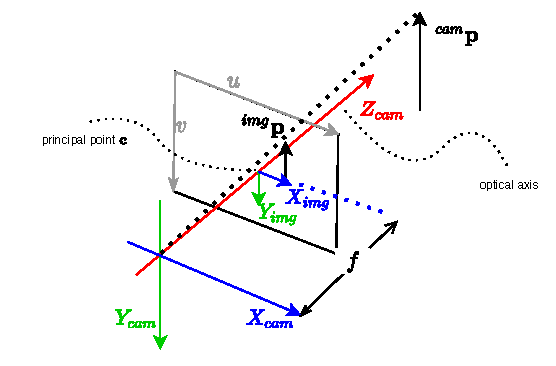
\includegraphics[width=0.75\textwidth]{figures/pinhole-cam.pdf}
\caption{\label{fig:pinhole-cam}The pinhole camera model results in a linear projection function, but typically this simplification comes at the cost of accuracy. The \(u\), \(v\) axes are the pixel-coordinate system whereas the \(X_{img}\), \(Y_{img}\) coordinate system is in world units and has its origin at the principal point \(\mathbf{c}\) where the optical axis intersects the image plane.}
\end{figure}

In its simplest form, the only parameters determining this function are the focal point of the camera \(f\) (the distance from the image screen to the point where the camera bundles light), and the principal point of the image \(\mathbf{c}\) (the point at which the lens axis intersects the image). 
Note that for digital images, the projected point needs to be mapped to the pixel-grid of the image plane (the coordinate frame spanned by \(u\) and \(v\)). 
The pixel dimensions \(p_x\), and \(p_y\) are necessary to compute the focal length and principal point coordinates from world units (i.e., meters) to image plane units (i.e., pixels) and hence discretize the projections. 
The resulting focal length and principal point components in pixel coordinates are denoted by subscripts of \(x\) and \(y\).
\cref{eq:pinhole-cam} shows this linearized projection:
\begin{equation}
\label{eq:pinhole-cam}
{}^{cam}p_z  \begin{pmatrix}p_u \\ p_v \\ 1 \end{pmatrix} = \begin{bmatrix}f_x & 0 & c_x \\ 0 & f_y & c_y \\ 0 & 0 & 1 \end{bmatrix}\begin{pmatrix}{}^{cam}p_x \\ {}^{cam}p_y \\ {}^{cam}p_z \end{pmatrix}
\end{equation}

Note that the z-coordinate of the Euclidean point scales the resulting image point in pixel coordinates. This scaling factor is a result of the fact that all points along the projective line connecting \({}^{cam}\mathbf{p}\) to \({}^{img}\mathbf{p}\) result in the same projected point \({}^{img}\mathbf{p}\). 
Consequently, this entails that one cannot recover the Euclidean point's depth from a projected point.

A model that allows for non-rectangular pixels introduces a skew-coefficient \(s=f_x\tan(\alpha)\) where \(\alpha\) is the angle between the \(x\) and \(y\) axes of the pixels (or, equivalently, the image) - see \cref{fig:skew-coeff} for a visualization of the skew coefficient.
The following equation extends the pinhole model to allow for a non-zero skew-coefficient:

\begin{equation}
\label{eq:pinhole-cam-skew}
{}^{cam}p_z\begin{pmatrix}p_u \\ p_v \\ 1 \end{pmatrix} = \begin{bmatrix}f_x & s & c_x \\ 0 & f_y & c_y \\ 0 & 0 & 1 \end{bmatrix}\begin{pmatrix}{}^{cam}p_x \\ {}^{cam}p_y \\ {}^{cam}p_z \end{pmatrix}
\end{equation}

\begin{figure}[htbp]
\centering
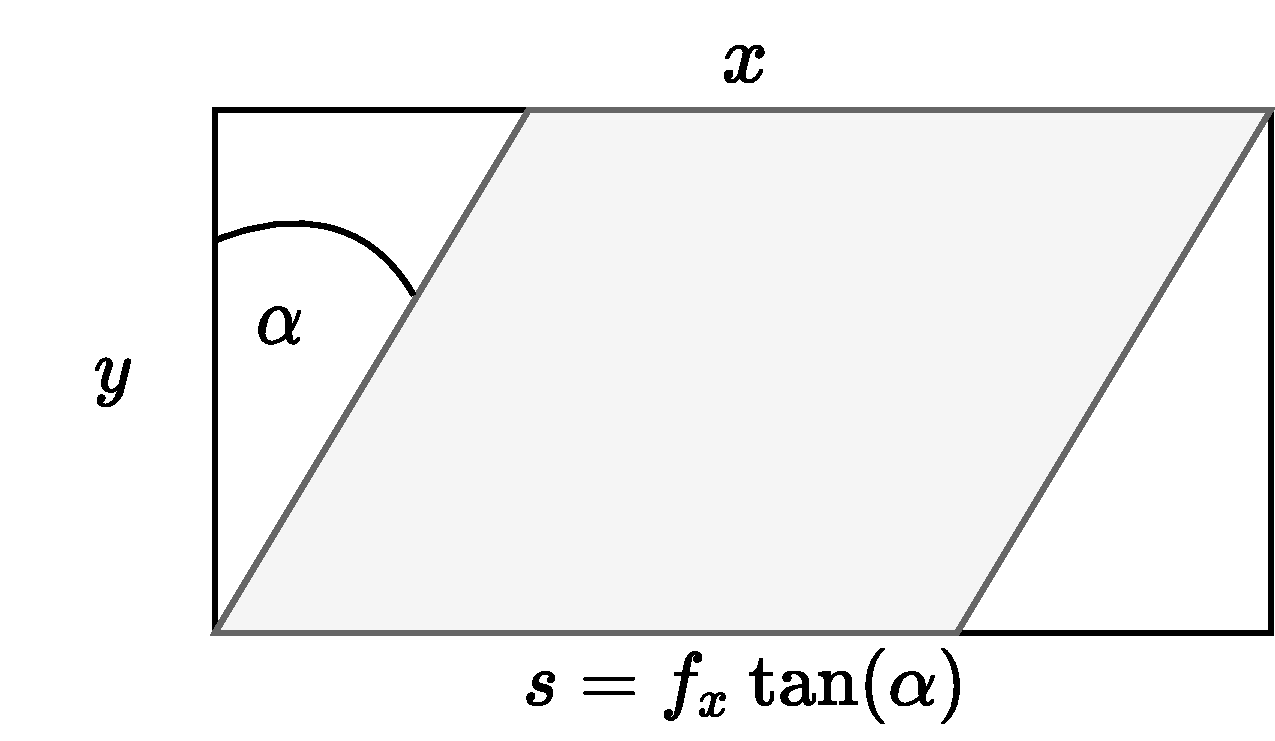
\includegraphics[width=0.5\textwidth]{figures/skew.pdf}
\caption{\label{fig:skew-coeff}The skew coefficient \(s\) measures the non-rectangularity of the pixels of a camera. Typically it is assumed to be 1 (i.e., pixels are rectangular). \(f_x\) is the x-component of the focal length vector in pixels.}
\end{figure}

Of course, this pinhole camera model is a highly idealized version of a projection function - real cameras do have lenses that result in various non-linear aberrations.
\cite{usenkoDoubleSphereCamera2018} presents an overview of camera models in use in real-world applications today. We will, however, only discuss the camera model utilized by this work.
This model is an extension of the pinhole camera allowing for radial and tangential distortion (see \cref{fig:distortion}) 
and is implemented by the computer vision library OpenCV\footnote{\url{https://www.github.com/opencv/opencv}} which we work with in this thesis.

\begin{figure}[htbp]
\centering
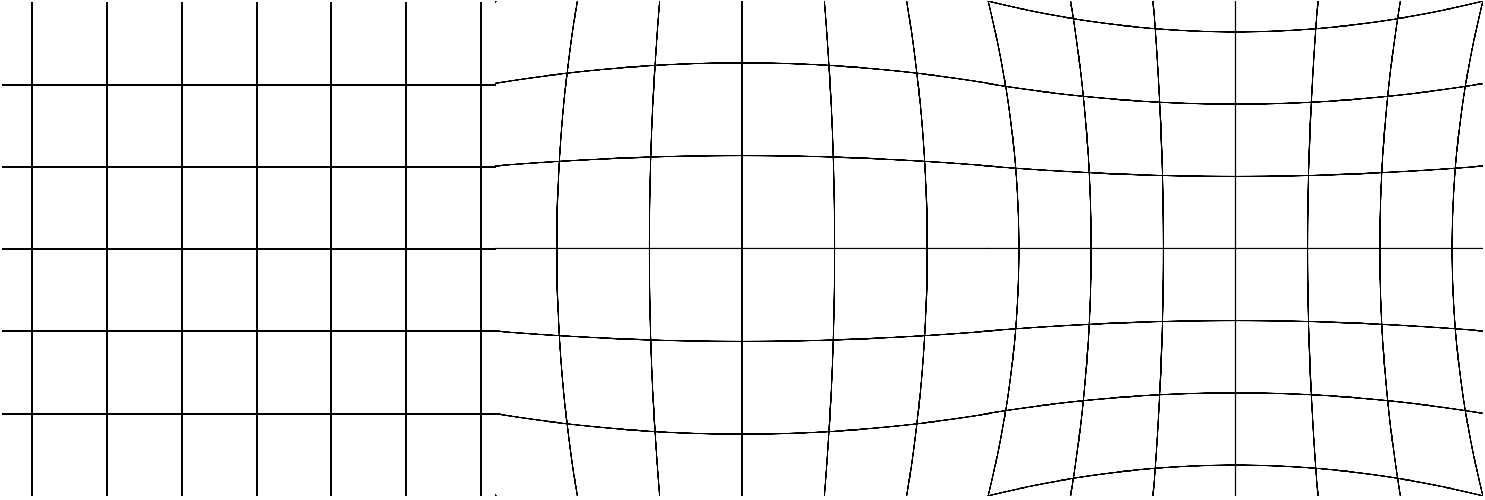
\includegraphics[width=.9\linewidth]{figures/distortion-types.pdf}
\caption{\label{fig:distortion}\emph{Left}: No distortion - lines in the coordinate grid are equally spaced. \emph{Middle}: Radial distortion - image lines converge outside of the image to form a barrel-like effect in the resulting image. \emph{Right}: Tangential distortion - image lines diverge outside of the image resulting in a ``pincushion''-type effect.}
\end{figure}

\newpage
As these two types of distortions introduce non-linearity into the projection function \(\pi(.)\), they can't be succinctly computed via matrix-vector multiplication but require the following steps:

\begin{equation}
\label{eq:cam-model}
\begin{split}
& p_x' = \frac{{}^{c}p_x}{{}^{c}p_z} \\
& p_y' = \frac{{}^{c}p_y}{{}^{c}p_z} \\
& r^2 = p_x'^2 + p_y'^2 \\
& p_x'' = p_x'\frac{1+k_1r^2+k_2r^4+k_3r^6}{1+k_4r^2+k_5r^4+k_6r^6} + 2t_1p_x'p_y'+t_2(r^2+2p_x'^2)\\
& p_y'' = p_y'\frac{1+k_1r^2+k_2r^4+k_3r^6}{1+k_4r^2+k_5r^4+k_6r^6} + 2t_2p_x'p_y'+t_1(r^2+2p_x'^2)\\
& p_u = f_x p_x'' + c_x \\
& p_y = f_y p_y'' + c_y
\end{split}
\end{equation}

In \cref{eq:cam-model} the radial distortion is influenced by the parameters \(k_i, i \in [1, 6]\) and the tangential distortion parameters by \(t_1\) and \(t_2\). Overall these parameters can be combined to 
\(\mathbf{d}^T = \begin{pmatrix}k_1&k_2&k_3&k_4&k_5&k_6&t_1&t_2\end{pmatrix}\).

The process of determining the parameters of the projection function (in our case, the intrinsic parameters \(\mathbf{A}\) - the focal length and principal point - and the distortion parameters \(\mathbf{d}\)) 
of an assumed camera-model is called camera calibration.
As the internal camera parameters typically do not change (for non-photographers), one needs to perform this process only once.

To calibrate a camera, one uses a so-called calibration object or rig. 
This calibration object is equipped with features easily extracted from and recognized in its projected image representation by pattern matching techniques not further discussed here.
The calibration object is typically planar (s.t. it is entirely spanned by two of the three dimensions) with repetitive patterns (see \cref{fig:calib-patterns} for an example of such an object) where the relative distance between elements of the pattern is known.

\begin{figure}[htbp]
\centering
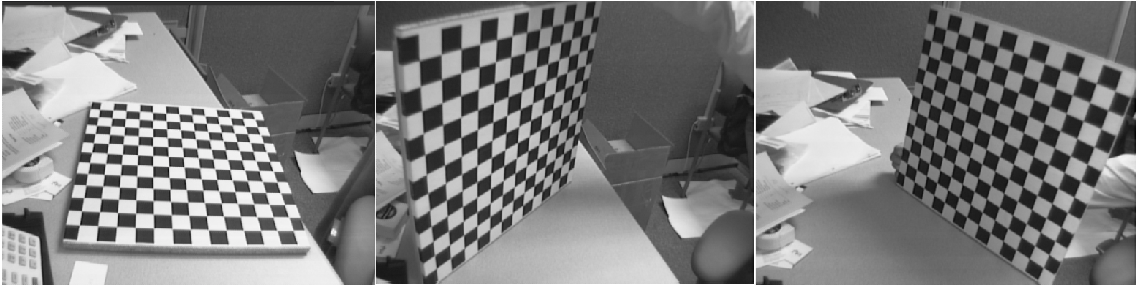
\includegraphics[width=0.8\textwidth]{figures/calib-patterns.pdf}
\caption{\label{fig:calib-patterns}Multiple images from different perspectives taken of a chessboard pattern used as a calibration object (images are freely available at \url{http://www.vision.caltech.edu/bouguetj/calib\_doc/htmls/calib\_example/index.html})}
\end{figure}

The object's origin is then either a uniquely recognizable feature or at some unique location w.r.t. the entire pattern.
This association process results in 2D-3D correspondences with known Euclidean points in the calibration object frame.
One now jointly estimates the extrinsic parameters (the camera pose w.r.t. the object frame), the intrinsic and distortion parameters (of the projection function) by projecting the calibration points to the image plane
and minimizing the distance of the projected points to the extracted feature locations. This distance is referred to as the reprojection error. 
Note that when using such planar calibration objects, at least two images of the object are necessary, and the accuracy of the estimated parameters increases with the number of images. 

Also, note that while a closed-form solution exists, noise in the projection and simplifications inherent to the model make a non-linear optimization objective preferrable \cite{zhangFlexibleNewTechnique2000}.
This non-linear least-squares objective is as follows and can be solved using an appropriate method, e.g. the Levenberg-Marquadt algorithm \cite{levenbergMethodSolutionCertain1944,marquardtAlgorithmLeastSquaresEstimation1963}: 

\begin{equation}
\label{eq:calib}
{}^w_c\mathbf{T}_i^*, \mathbf{A}^*, \mathbf{d}* = \text{argmin}~\frac{1}{2} \sum_{i=0}^{n_{images}}\sum_{j=0}^{n_{features}}||\begin{pmatrix}f^{ij}_u \\ f^{ij}_v \end{pmatrix} - \pi(({}^w_c\mathbf{T}_i)^{-1}{}^w\mathbf{p}^{j}, \mathbf{d}, \mathbf{A})||^2_2
\end{equation}

\(f^{ij}_{\{u, v\}}\) in \cref{eq:calib} are the feature coordinates of feature \(j\) in image \(i\), \({}^w\mathbf{p}^{j}\) is the associated object point, and \({}^w_c\mathbf{T}_i\) the relative camera-object pose at image \(i\).

Minimization of this objective then leads to a known projective function necessary for the following steps of recovering 3D scene information.
The inverse of the projection function \(\pi(.)\) ``back-projects'' a point from the image plane to camera coordinates and is the ray through all Euclidean points which project to the same image points.

\subsection{Epipolar Geometry \label{epipolar-geometry}}
\label{sec:org81b8b23}
    Now that we have calibrated cameras, the remaining piece enabling 3D reconstruction is the geometry between these two cameras.
The intrinsic parameters of both cameras as well as the relative rigid body transformation \({}^r_l\mathbf{T} \in  SE(3)\) from the left to the right camera entirely define this relationship. 
\cref{fig:epipolar-geom} shows a general configuration of such a stereo setup. 

Note that the given configuration and following discussion assumes a pinhole-camera model (as described in the previous section) where both cameras have the same intrinsic matrix \(\mathbf{A}\).
Additionally, the virtual image plane (upright, between object and camera) is considered instead of the real, inverted image plane behind the camera (as was done in \cref{fig:pinhole-cam}).

\begin{figure}[htbp]
\centering
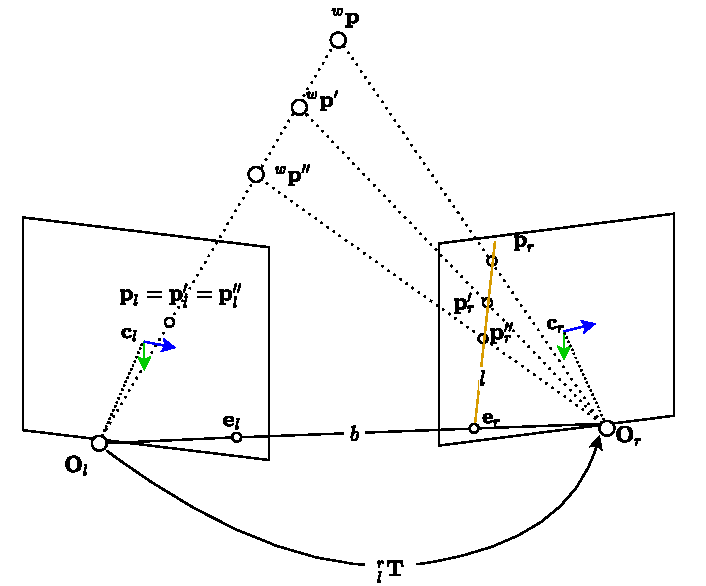
\includegraphics[width=0.7\textwidth]{figures/epipolar-geom.pdf}
\caption{\label{fig:epipolar-geom}The epipolar geometry between two pinhole-cameras. A point projects via the optical centers to the image planes of both cameras.}
\end{figure}


When projecting some arbitrary scene point \({}^w\mathbf{p}\) (seen by both cameras) to the left and right image planes, this results in two 2D points 
\(\mathbf{p}_l\) and \(\mathbf{p}_r\), respectively. Due to the linearity of the projection function, the line, or ray, passing through the 3D point and the
respective image points also passes through the camera's corresponding optical centers \(\mathbf{O}_l\) and \(\mathbf{O}_r\). As these rays are (for objects at finite distances)
not parallel and, generally, \(\mathbf{O}_l \neq \mathbf{O}_r\), all points along these rays through \(O_{\{l, r\}}\) project to a single point in the corresponding image plane: \(\mathbf{p}^0_{\{l, r\}}\). 
However, on the respective other image, the points along these rays \(\mathbf{r}_{\{l, r\}}\) project to a line \(l_{\{r, l\}}\). This line is called the epipolar line. 
All epipolar lines on one image plane intersect at the epipolar point \(\mathbf{e}_{\{l, r\}}\). One can also construct these epipolar points by projecting one camera's optical center to the other's image plane. Furthermore, these two projection rays coincide, i.e., there is a line going through both optical centers and both epipolar points.
This line is often referred to as the baseline \(b\). The plane constructed from the baseline and the rays \(\mathbf{r}_{\{r, l\}}\) is called the epipolar plane.
From the notion of an epipolar line, the so-called epipolar constraint follows \cite{hartleyMultipleViewGeometry2004}: 
if one knows the geometry between two cameras and wants to find a given point from the left image in the right image, one can restricts one's search to the right image's corresponding epipolar line.
Put differently, transforming the left ray \(\mathbf{r}_l\) to the right coordinate system (i.e., \({}^r_l\mathbf{R}\mathbf{r}_l + {}^r_l\mathbf{t}\)) and taking the cross-product of this 
transformed ray and the baseline (which is identical to \({}^r_l\mathbf{t}\)) produces a vector normal to the epipolar plane. 
\begin{equation}
{}^r_l\mathbf{t} \times ({}^r_l\mathbf{R}\mathbf{r}_l + {}^r_l\mathbf{t}) = {}^r_l\mathbf{t} \times {}^r_l\mathbf{R}\mathbf{r}_l
\end{equation}
Thus, taking the dot-product of this vector and the right ray must be zero (as these must also be perpendicular): 
\begin{equation}
\mathbf{r}_r \cdot ({}^r_l\mathbf{t} \times {}^r_l\mathbf{R}\mathbf{r}_l) = 0
\end{equation}
As the projected points are proportional to the rays (and utilizing the cross-product to skew-symmetric transformation introduced in \cref{transformations-3d}) the previous equation simplifies to:

\begin{equation}
\label{eq:epipolar-constraint}
\mathbf{p}_r^T ({}^r_l\mathbf{t}^\wedge {}^r_l\mathbf{R})\mathbf{p}_l = \mathbf{p}_r^T \mathbf{E} \mathbf{p}_l = 0
\end{equation}

\(\mathbf{E}\) in \cref{eq:epipolar-constraint} is called the essential matrix and captures the relative transformation between the two cameras.

The epipolar constraint formulated by \cref{eq:epipolar-constraint} now allows estimating the essential matrix given sufficient point correspondences between the left and right images. 
This estimation can be done with the Eight-Point Algorithm \cite{longuet-higginsComputerAlgorithmReconstructing1981,hartleyDefenseEightpointAlgorithm1997} given - as the name suggests - at least eight point pairs.

Typically, one calibrates the intrinsic parameters of each camera and the relative extrinsic calibration between cameras conjointly. 

A special case of the epipolar geometry is the so-called epipolar standard configuration (see \cref{fig:epipolar-standard}): 
here, both image planes lie in the same plane, s.t. all epipolar lines are parallel to each other (and the baseline), and the epipoles lie at infinity. 

\begin{figure}[htbp]
\centering
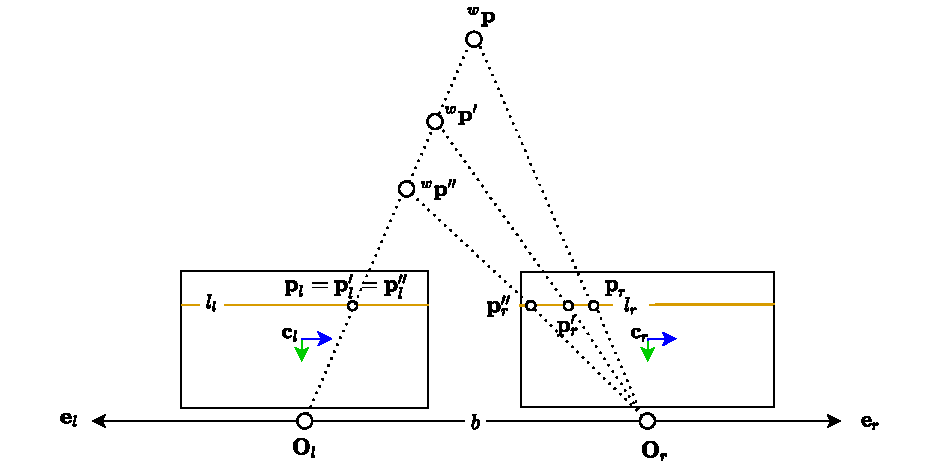
\includegraphics[width=.9\linewidth]{figures/epipolar-standard.pdf}
\caption{\label{fig:epipolar-standard}In the epipolar standard configuration, both image planes lie in the same plane, making the epipolar lines parallel as the epipoles lie at infinity.}
\end{figure}

This configuration is especially desirable when searching for the corresponding point in the other image by exploiting the epipolar constraint:
the configuration constrains the search to a single row in the image plane for which efficient implementations exist. 
Additionally, if one has a calibrated stereo camera system, one can compute the rotation matrices necessary to transform both image planes to the epipolar standard configuration. From this, one can also transform the images so that they display the desired configuration, and their epipolar lines are parallel. 
\cite{hartleyMultipleViewGeometry2004} explains this process known as image rectification.

\newpage
\subsection{Stereo Triangulation \label{triangulation}}
\label{sec:orgff4bed2}
    Knowing the intrinsics of both cameras and the relative transformation between them now allows us to recover the lost depth information from a left-right pair of projected points.
This procedure is known as triangulation: given two corresponding points  \(\mathbf{p}_l\) and \(\mathbf{p}_r\) from left and right images, respectively, the point where the ``back-projected'' 
rays \({}^r\mathbf{r}\) and \({}^l\mathbf{r}\) intersect is the underlying 3D point \({}^c\mathbf{p}\).
However, due to many noise sources (discretized image plane, lenses, etc.), these rays mostly do not intersect (\cref{fig:triangulation} illustrates this).
In the most general sense (i.e., when the projection functions \(\pi_{\{l, r\}}(.)\)) of the cameras are non-linear) one can solve triangulation by posing the problem as a non-linear least squares problem 
and using e.g. Gauss-Newton \cite{bjorckNumericalMethodsLeast1996} to minimize the reprojection errors:

\begin{equation}
\label{eq:triangulation-non-linear}
\min_{{}^w\mathbf{p}} \sum_{i \in \{l, r\}}||\mathbf{p}_i - \pi({}^i_w\mathbf{T}{}^w\mathbf{p})||_2^2
\end{equation}

\({}^w\mathbf{p}\) is really the point in the left camera coordinate system as we only know the relative transformation \({}^l_r\mathbf{T}\) s.t. \({}^w_l\mathbf{T} = \mathbf{I}^4\) and \({}^w_r \mathbf{T} = {}^l_r\mathbf{T}\). 

If the projection functions are linear (i.e., given by the extrinsic camera poses and intrinsic camera matrices), one can also pose triangulation as a regular least-squares problem.

\begin{figure}[htbp]
\centering
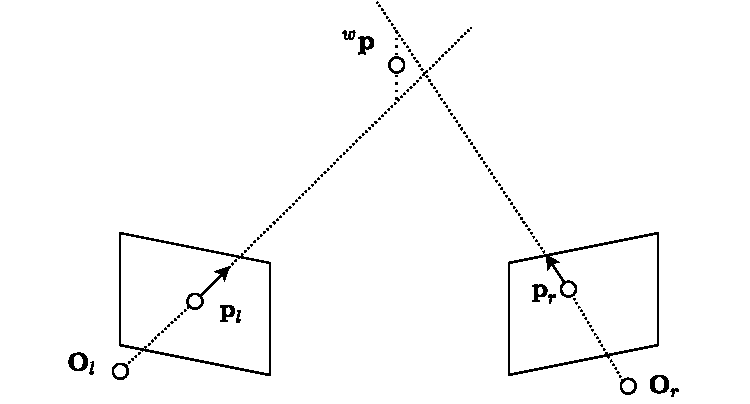
\includegraphics[width=0.7\textwidth]{figures/triangulation.pdf}
\caption{\label{fig:triangulation}In the presence of noise, the two projection rays for a pair of projected points do not intersect. An estimate of the 3D location is then the middle of the shortest path connecting these two rays.}
\end{figure}


\subsection{RANSAC \label{ransac}}
\label{sec:org68c2884}
    Dealing with noise is a challenge for any task that involves real-world data from imperfect sensors or applies simplified assumptions about said's data underlying model.
Estimating a model's parameters using noisy data will especially result in errors if the noise is not uniform across all data points.
Under this assumption, one can divide the data points into two subsets: data supporting a model (within a certain noise threshold), dubbed inliers, and outliers - data corrupted by extreme noise which holds no information about the parameters to be estimated.
\gls{ransac} is a popular method developed in the early 1980s for robust model estimation \cite{fischlerRandomSampleConsensus1981}.
\gls{ransac} is an iterative process that consists of the following two steps and terminates when a stopping criterion is met:

\begin{enumerate}
\item Randomly select a minimum amount of \(n\) points (hypothetical inliers) from the data from which the model parameters can be estimated and fit the model to these
\item Determine the number of points that support this model (the consensus set), i.e., their deviation w.r.t. the model falls within a given threshold
\end{enumerate}

The stopping criteria are: the consensus set must reach a threshold, or the number of iterations must exceed some maximum. The values of these criteria are application-specific.
Typically, if the procedure reaches the maximum number of iterations without crossing the inlier ratio (i.e., inliers over total points), the estimation is considered failed.
If, however, the process finishes successfully, the model can then be re-estimated on the entire consensus set leading to more robust parameters.

Generally, there is no guarantee that \gls{ransac} finds the inlier set. At every iteration, \(n\) points are selected uniformly from the entire dataset.
Given a ground truth inlier ratio \(t_i = \frac{n_i}{n}\) where \(n_i\) are the number of inliers, the probability of selecting \(n\) inlier points
in a single iteration is \((t_i)^n\) and, conversely, the probability of selecting at least one outlier is \(1-(t_i)^n\). Assuming for simplicity that a single
outlier in the hypothetical inlier set will result in a model that doesn't reach the required inlier ratio, it follows that the probability of selecting non-inlier sets for \(k\) consecutive iterations is \((1-(t_i)^n)^k\). This result now allows one to set the maximum iterations \(k_{max}\) by choosing a probability \(p\) for
successful completion of the process. The converse probability of failure is then \(1-p\) and equating the previously deduced probability of failure after \(k\) iterations
to this, i.e., 
\begin{equation}
 (1-(t_i)^n)^k=1-p
\end{equation}
we get 
\begin{equation}
k_{max} = \frac{\log(1-p)}{\log(1-(t_i)^n)}
\end{equation}
As previously mentioned, this deduction assumes that a single outlier in an inlier set will distort the resulting model to the point of failure. Therefore, \(k_{max}\) can be seen as an upper bound. Additionally, the inlier threshold \(t_i\) is generally unknown s.t. it makes sense to use a low estimate for this (and consequently compute a larger \(k_{max}\)).


An example of a (for simplicity, single iteration) \gls{ransac} scheme for fitting a linear function is given in \cref{fig:ransac}.

\begin{figure}[htbp]
\centering
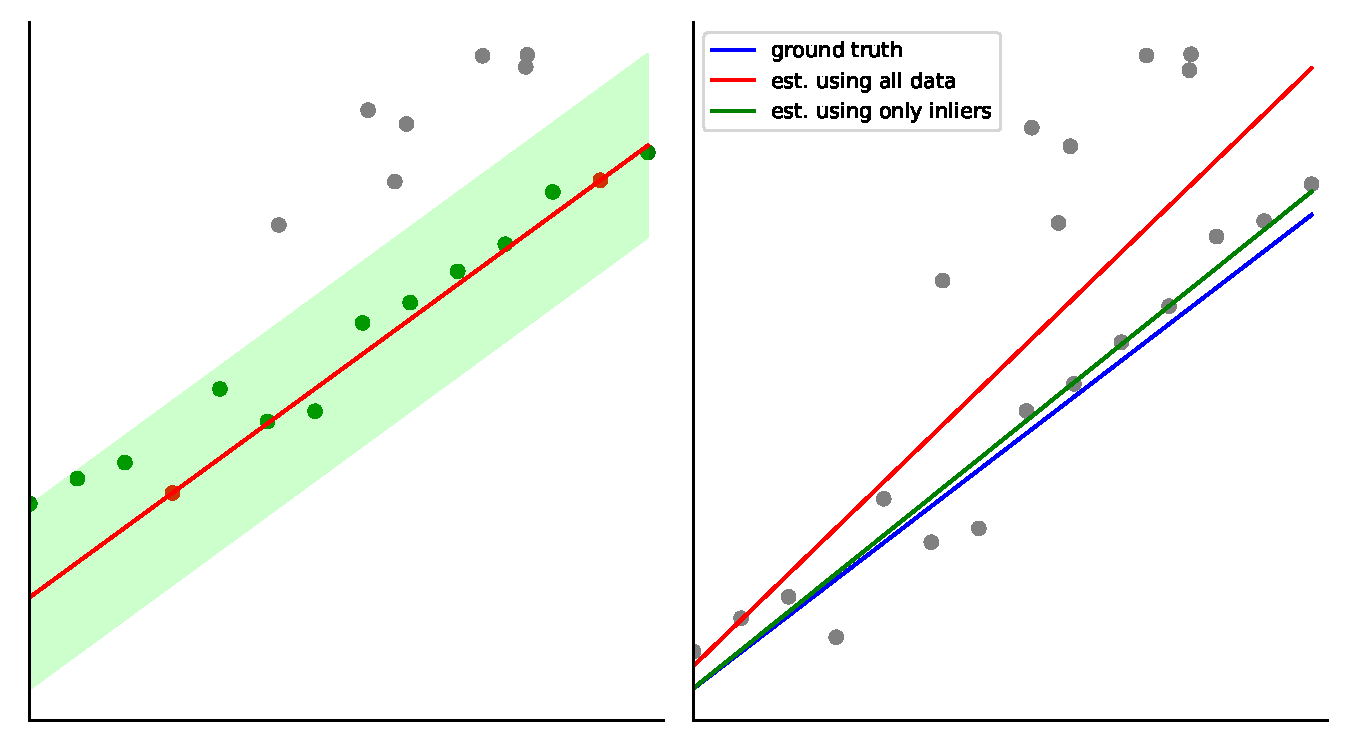
\includegraphics[width=0.7\textwidth]{figures/ransac.pdf}
\caption{\label{fig:ransac}\emph{Left:} A single iteration of a RANSAC scheme on a dataset distorted by outliers (gray) assuming a linear model. Two points (red) are used to estimate the model (red line) and the consensus set (green) are all points within a certain threshold (green area). \emph{Right}: The same set and the underlying ground truth function (blue), the estimated function using the entire consensus set (green) and the estimated function using all datapoints (red). \emph{Best viewed in color.}}
\end{figure}

\subsection{Perspective-n-Point Camera Pose Estimation \label{pnp}}
\label{sec:org28140c1}
    Given a set of known 3D points and their corresponding projected points on an image plane, the extrinsic pose \({}^w_c\mathbf{T} \in SE(3)\) can be estimated via a process known as \gls{pnp} \cite{longquanLinearNpointCamera1999}.
Generally, the problem is similar to the triangulation problem described in \cref{triangulation}, the difference being that we only have a single camera with an unknown pose and multiple Euclidean points with known coordinates.
Still, for \(n\) 2D-3D correspondences the generalized non-linear minimization objective looks familiar:

\begin{equation}
\label{eq:pnp}
\min_{{}^c_w\mathbf{T}} \sum_i^n||\mathbf{p}_i - \pi({}^c_w\mathbf{T}{}^w\mathbf{p}_i)||_2^2
\end{equation}

The desired pose has six \glspl{dof} and, hence, a non-linear solver for \cref{eq:pnp} requires a good initialization for convergence.

However, several linear solutions exist, the earliest dating back as far as 1841 \cite{longquanLinearNpointCamera1999}. 
At a minimum, \gls{pnp} needs three points to solve the problem. This approach is called P3P \cite{xiao-shangaoCompleteSolutionClassification2003}. 
However, using three points results in four feasible solutions. Adding a fourth point can resolve the ambiguity.
A linear approach using \gls{dlt} as a solver exists as well.

The arguably most common procedure for solving the \gls{pnp} problem is \gls{epnp} and was published in 2008 by Lepetit et al. \cite{lepetitEPnPAccurateSolution2009}.
This method solves the non-linear least-squares from \cref{eq:pnp} via Gauss-Newton but initially estimates the rotational and translational components by expressing the world points as linear combinations. The factors are shared across points and termed virtual points. The resulting problem is that of estimating these control points on the image plane.

As outliers (i.e., incorrect 2D-3D correspondences) are a common problem in the \gls{pnp} scenario, one commonly applies a \gls{ransac} scheme to the estimation (as detailed in \cref{ransac}).

\section{SLAM \label{slam}}
\label{sec:org0e0d7d6}
   \gls{slam} is the process by which a robot, car, or even hand-held device uses its sensors to build a model of its surroundings and to localize itself in it simultaneously - 
without having any a priori information of its environment. 

\subsection{Early SLAM solutions}
\label{sec:org07866cc}
That is, the \gls{slam} problem consists of an ego or camera trajectory made up of \(n\) poses \({}^w_c\mathbf{T}_i \in SE(3) ~\text{with}~ i \in [1, n]\) and \(m\) Euclidean points 
(so-called landmarks \(\mathbf{l} = \{\mathbf{l}_1, \mathbf{l}_{2}, ..., \mathbf{l}_m\}\)) that describe the map. 

Each landmark \(\mathbf{l}_i\), in turn, has \(k\) measurements or observations \(\mathbf{o}^i = \{\mathbf{o}^i_1, \mathbf{o}^i_2, ..., \mathbf{o}^i_k\}\) associated with it. 

The set of all observations is then \(\mathbf{o} = \{\mathbf{o}^1, \mathbf{o}^2, ..., \mathbf{o}^m\}\).
Additionally, landmarks may hold supplementary information (e.g. an RGB-color value or a descriptor - see \cref{feature-points}).

Generally, the problem for a single time-step \(t\) can be stated probabilistically as the following posteriori probability encompassing the ego-pose and landmarks:

\begin{equation}
\label{eq:slam-prob}
P({}^w_c\mathbf{T}_t, \mathbf{l} | {}^w_c\mathbf{T}_0, \mathbf{o}_{0:t})
\end{equation}

In \cref{eq:slam-prob}, \(\mathbf{o}_{0:t}\) denotes all landmark observations made up until the current time-step. 

The first \gls{slam} systems were developed by the mobile-robotics community in the 1990s and early 2000s, e.g. \cite{leonardSimultaneousMapBuilding1991,guivantLocalizationMapBuilding2000,gutmannIncrementalMappingLarge1999,10.5555/777092.777184}.

These early approaches solve the \gls{slam} problem either via linear-filtering \cite{leonardSimultaneousMapBuilding1991} (i.e., with \glspl{ekf} - see \cite{brownIntroductionRandomSignals1997} for a discussion on Kalman filters), 
non-linear filtering (i.e., with Rao-Blackwellized particle filter \cite{10.5555/777092.777184}), or through \glspl{mle} \cite{cadenaPresentFutureSimultaneous2016}. 
Generally, these formulations encode the system state (poses \& landmarks) in a single vector and extended the formulation given in \cref{eq:slam-prob} to include knowledge of a robot's control inputs 
\(\mathbf{{u} = \{\mathbf{u}_1, \mathbf{u}_2, ..., \mathbf{u}_n\}}\):

\begin{equation}
\label{eq:slam-prob-ctrl-input}
P({}^w_c\mathbf{T}_t, \mathbf{l} | {}^w_c\mathbf{T}_0, \mathbf{o}_{0:t}, \mathbf{u}_{0:t})
\end{equation}

A central realization of research of the \gls{slam} problem conducted in the wake of the success of these early systems was that the errors of landmarks observations and pose estimates for a single timestep 
are highly correlated and, hence, result in a much more sparse, and thus numerically superior, problem than initially assumed \cite{cadenaPresentFutureSimultaneous2016}. 

\subsection{Solving SLAM via MAP}
\label{sec:orgc0908ab}
The current standard solution (leaving out control inputs for simplicity) to solving \gls{slam} is via \gls{map}:
\begin{equation}
\label{eq:slam-map}
{}^w_c\mathbf{T}_t^*, \mathbf{l}* = \argmax_{{}^w_c\mathbf{T}_t, \mathbf{l}} P({}^w_c\mathbf{T}_t, \mathbf{l} | {}^w_c\mathbf{T}_0, \mathbf{o}_{0:t})
\end{equation}

Combining poses and landmarks to a single state-vector \(\chi_t\), applying Bayes' Theorem and assuming non-correlated measurements between timesteps, we arrive at 

\begin{equation}
\label{eq:slam-map-2}
\chi_t^* = \argmax_{\chi_t} P(\chi_t) \prod_{k=1}^{t}P(\mathbf{o}_{0:k} | \chi_k)
\end{equation}

Further assuming zero-mean Gaussian distribution of measurement noise, an underlying function \(h(.)\) mapping landmarks-poses combinations to the measurement space, and utilizing the fact that
maximizing a Gaussian-distributed function is equivalent to minimizing the negative \(\log\) of it, we arrive at the following least-squares problem (see \cite{cadenaPresentFutureSimultaneous2016} for a step-by-step derivation):

\begin{equation}
\label{eq:slam-map-ls}
\chi_t^* = \argmin_{\chi} \sum_{k=0}^t||h(\chi_k) - \mathbf{o}_{0:k}||_2^2
\end{equation}

As with previously presented least-squares problems (see \cref{camera-calibration} and \cref{triangulation}), non-linear solvers such as Gauss-Newton or Levenberg-Marquardt can solve this.
Many implementations exploit the sparsity, as mentioned earlier, of the problem to solve it more efficiently.

Another critical aspect of \gls{slam} is global map consistency. The process of ensuring such consistency is known as loop-closure and entails recognizing previously-seen places and updating the map once such a closure is detected.
Loop-closure is necessary for accurate map and pose estimates as even minor estimation errors will accumulate over time to result in large so-called drift errors.
\cref{fig:loop-closure} illustrates such a drift and the result of a successful loop-closure.

\begin{figure}[htbp]
\centering
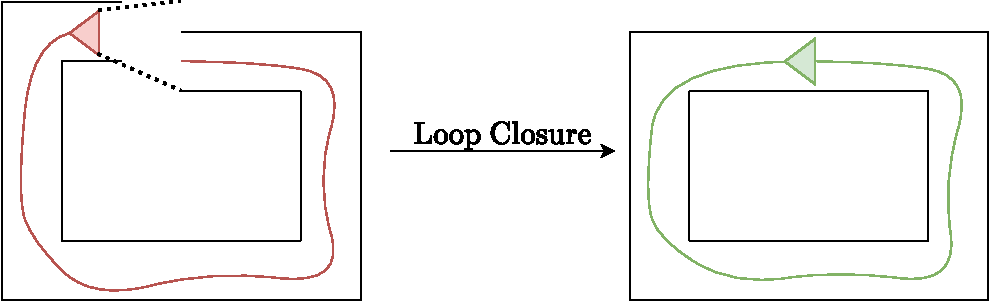
\includegraphics[width=.9\linewidth]{figures/loop-closure.pdf}
\caption{\label{fig:loop-closure}Loop closure enables globally consistent maps via place recognition (left) and consequent map and pose adjustments (right).}
\end{figure}


\subsection{Visual SLAM \label{visual-slam}}
\label{sec:org4622bdd}

    Although \gls{slam} has its origin with robots equipped with \gls{lidar} or SONAR sensors, the success of recreating 3D representations of scenes from a collection of 
unordered images taken from different viewpoints \cite{agarwalBuildingRomeDay2011} (known as \gls{sfm}) motivated the use of RGB-cameras as input for \gls{slam} systems. 
Different approaches exist here as well: either utilizing pixel-intensity data directly \cite{engelLSDSLAMLargeScaleDirect2014,engelDirectSparseOdometry2018} or via indirect feature points (see \cref{feature-points})\cite{mur-artalORBSLAMVersatileAccurate2015a,mur-artalORBSLAM2OpenSourceSLAM2017} extracted from the images.
For the later approach this leads to the following updated optimization objective from \cref{eq:slam-map-ls} (where \(\mathbf{o}_{t}^{m}\) is the image point associated to/measured as landmark \(\mathbf{l}_m\) at timestep \(t\)):

\begin{equation}
\label{eq:slam-map-visual}
    {}^w_c\mathbf{T}_t^*, \mathbf{l}^* =  \argmin \sum_{t, m}||\mathbf{o}_{t}^{m} - \pi({}^{o}_{c}\mathbf{T}^{t}{}^{o}\mathbf{l}_{m})||^2
\end{equation}


\cref{eq:slam-map-visual} is very similar to the optimization procedure in \gls{sfm} known as \gls{ba}. However, it differs in that \gls{sfm} does this optimization globally, whereas \gls{slam} is inherently iterative - optimizing at each step.
Nonetheless, we will refer to this optimization in visual \gls{slam} as \gls{ba}.


A final important measure for \gls{slam} systems is that they aim to operate in real-time. Although the problem is sparse, the number of variables grows exponentially with the number of frames, and, hence, 
one must apply techniques to constrain the optimization problem's dimensionality.
One typically achieves this by choosing measurements to keep or discard and running the optimization only on a subset of the measurement data, e.g., by removing redundant or outlier poses and landmarks.
The arguably most notable addition to visual \gls{slam} systems is ORB-SLAM \cite{mur-artalORBSLAMVersatileAccurate2015a,mur-artalORBSLAM2OpenSourceSLAM2017}.
This system introduces a so-called covisibility graph to ``window'' the optimization by only considering local frames.
Informally, at some time \(t\) only poses and landmarks are included in the optimization if they are part of or see, respectively, the local scene viewed by the camera at time \(t\).

\chapter{Related Work \label{related-work}}
\label{sec:orgfc14dd9}
  This work builds upon state-of-the-art \gls{dl} object detection (see \cref{modat}) and the tried-and-tested graph-optimization technique, i.e., \gls{ba}, from \gls{slam} (see \cref{slam} and \cref{visual-slam}).
Although this work's focus is on 3D \gls{mot}, the ``bigger-picture'' goal is to incorporate the proposed system with a static \gls{slam} system to facilitate dynamic scene understanding.
Thus, this chapter will review systems that have incorporated object detection or object tracking to improve \gls{slam} performance without implementing a \gls{mot} system.
Next, the chapter discusses metrics that try to quantify \gls{mot} performance, and finally, existing 3D \gls{mot} (with and without \gls{slam} incorporation) are presented.


\section{Dynamic SLAM \label{dynamic-slam}}
\label{sec:org5a49cdd}
   Classical \gls{slam} systems fail to differing degrees in highly dynamic environments based on a static-world assumption. However, the capability of dealing with such surroundings is paramount in moving towards robust autonomous navigation outside of empty factory floors. 
There exist several approaches which either detect objects, e.g., \cite{yuDSSLAMSemanticVisual2018,bescosDynaSLAMTrackingMapping2018,salas-morenoSLAMSimultaneousLocalisation2013}, or more generally, 
dynamic parts of the environment, e.g., \cite{liRGBDSLAMDynamic2017}, and then remove the associated areas from the sensor input to improve ego-tracking and static map creation.

\cite{salas-morenoSLAMSimultaneousLocalisation2013} introduce an ``object-oriented'' approach to \gls{slam} for environments with a priori knowledge of object types that are likely present in a given scene. The RGB-D system then detects
objects and matches them via \gls{icp} to 3D models in a database. The proposed systems removes object areas of the RGB-D frame from the static map pose-graph optimization. 
The authors claim improved performance compared to previous systems, especially w.r.t. scene geometry; however, they only show qualitative results.
Li and Lee \cite{liRGBDSLAMDynamic2017} presents a system that divides an RGB-D depth map into static and dynamic points. The authors accomplish this by transforming the previous map to its expected
representation via an estimated ego-motion. They then perform \gls{icp} between this estimated map and the current depth map and discard collections of points whose Euclidean distance is greater than some threshold (they call these ``dynamic edges'').
The authors evaluate their system on the indoor TUM dataset \cite{sturmBenchmarkEvaluationRGBD2012} and compare their ego-tracking to the current state-of-the-art RGB-D-based visual odometry (i.e., no loop-closure)
 systems \cite{kerlRobustOdometryEstimation2013,kimEffectiveBackgroundModelBased2016} and show significant improvement of ego-tracking in highly dynamic environments. 
Additionally, they exhibit improved performance compared to the at-the-time state-of-the-art non-real-time RGB-D \gls{slam} system \cite{sunImprovingRGBDSLAM2017}.

Another system that excludes objects from the \gls{slam} optimization problem is DynaSLAM \cite{bescosDynaSLAMTrackingMapping2018}. 
The authors present monocular, stereo and RGB-D flavors of their system. In their proposal, the authors detect objects via the state-of-the-art object detector MaskR-CNN \cite{heMaskRCNN2018}.
In the RGB-D case, they additionally use multi-view geometry assumptions to enhance the detected object (e.g., the book a person is holding is included in the final dynamic object although it was not part of the MarkR-CNN detection).
The system then excludes those dynamic parts of the frame when optimizing the ego-pose and static map. 
Furthermore, they estimate the masked frame-parts from the existing static map and output an ``inpainted'' frame without the dynamic objects.
The authors evaluate their system on the TUM \cite{sturmBenchmarkEvaluationRGBD2012} and KITTI \cite{geigerVisionMeetsRobotics2013} datasets and compare ego-tracking of their system to ORB-SLAM \cite{mur-artalORBSLAMVersatileAccurate2015a}.
DynaSLAM proves to be much more robust than ORB-SLAM in dynamic environments.

DS-SLAM \cite{yuDSSLAMSemanticVisual2018} follows a similar approach to DynaSLAM. Yu et al. extend ORB-SLAMv2 \cite{mur-artalORBSLAM2OpenSourceSLAM2017} to more robustly handle dynamic environments.
The authors achieve this by introducing a semantic segmentation network (SegNet \cite{badrinarayananSegNetDeepConvolutional2017}) which detects objects. They then exclude the detected objects from the input frame for ORB-SLAMv2.
Additionally, for detected features, they perform an optical-flow-based check to determine whether a feature has moved significantly between frames and if so, regard the feature as an outlier.
They then compare their system to ``vanilla'' ORB-SLAMv2 on the RGB-D TUM dataset \cite{sturmBenchmarkEvaluationRGBD2012} and show one order-of-magnitude improvement in ego-tracking accuracy for highly dynamic scenes.

The relatively recent ClusterSLAM \cite{huangClusterSLAMSLAMBackend2019} assumes no a priori knowledge of object types or topologies. Instead, it clusters objects based on groups of landmarks that show similar relative motion
between frames. This procedure results in clusters for each object as well as a cluster for the static map. All landmarks clusters are then optimized via \gls{ba} independently; ego-motion is estimated from the static cluster.
The authors show that disjunct optimization of clusters outperforms a single optimization objective that combines all clusters. Although objects are tracked, the authors only show
improved ego-tracking and landmark location estimates compared to \cite{mur-artalORBSLAM2OpenSourceSLAM2017,bescosDynaSLAMTrackingMapping2018,reddyCarFusionCombiningPoint2018,muraliUtilizingSemanticVisual2018} 
on synthetic indoor and outdoor scenes created via \cite{songSemanticSceneCompletion2016} and \cite{dosovitskiyCARLAOpenUrban2017}. 

Another issue specific to monocular visual \gls{slam} is that of scale ambiguity. RGB-D systems or stereo cameras do not suffer from this as they either directly (RGB-D) or indirectly (the baseline between stereo cameras)
deduce world points in meters. However, \cite{frostRecoveringStableScale2018} shows that detecting objects with a known scale can diminish this scale ambiguity for monocular setups. 
The presented system detects and tracks cars by detection (based on \cite{zhangUnderstandingHighLevelSemantics2013} and \cite{geiger3DTrafficScene2014}) of 2D bounding boxes. 
It represents objects by a center point and a fixed dimension (i.e., a cube around a center point). This center is then included in the graph-optimization problem to recover scale. Additionally, points in regions of detected objects are not used as static map features. Note that the system is only able to deal with stationary objects and fails to track moving vehicles.
The authors compare performance on the KITTI dataset \cite{geigerVisionMeetsRobotics2013} of their \gls{slam} system with and without including objects in their graph-optimization.
They show that the inclusion of this prior scale knowledge immensely reduces the scale error.

The presented research unambiguously demonstrates that a 3D \gls{mot} system that can mask sensor input for an existing static \gls{slam} system will result in the latter's improvement.

\section{Combining SLAM and Multi-Object Tracking}
\label{sec:orgbe2e88c}
There exist several works which combine visual \gls{slam} and \gls{mot} \cite{liStereoVisionbasedSemantic2018,heneinDynamicSLAMNeed2020,barsanRobustDenseMapping2018,yangCubeSLAMMonocular3D2019,dongVisualInertialSemanticSceneRepresentation2017}.

Dong et al. \cite{dongVisualInertialSemanticSceneRepresentation2017} propose a system that decouples the \gls{slam} and the \gls{mot} subsystems.
For performing ego-tracking and static map creation, the authors utilize \cite{tsotsosRobustInferenceVisualinertial2015} for their non-real-time and \cite{mur-artalORBSLAMVersatileAccurate2015a} for their real-time capable version. 
Their implementation describes objects by a pose \(\in SE(3)\) and an a priori assumed shape. 
The authors detect and track objects via an \gls{ekf}, a combination of a \gls{dl} object detector (SubCNN \cite{xiangSubcategoryawareConvolutionalNeural2017} for the non-real-time version and YOLO \cite{redmonYouOnlyLook2016} otherwise) and the object's class and pose.
The resulting system is evaluated on 3D object detection (not tracking) accuracy on the KITTI dataset \cite{geigerVisionMeetsRobotics2013} and compared to ``vanilla'' SubCNN \cite{xiangSubcategoryawareConvolutionalNeural2017} which it outperforms. 

In contrast to the previous system, CubeSLAM \cite{yangCubeSLAMMonocular3D2019} proposes a sparse feature-based approach that tightly couples \gls{slam} and \gls{mot} s.t. both systems benefit from each other.
First, objects are detected via \cite{redmonYouOnlyLook2016} for indoor scenes or \cite{caiUnifiedMultiscaleDeep2016} for outdoor scenes.
Concurrently, a static \gls{slam} system based on ORB-SLAMv2 \cite{mur-artalORBSLAM2OpenSourceSLAM2017} estimates the ego-pose.
Detections are associated with existing object tracks by estimating existing tracks' positions via optical flow and performing 2D \gls{iou} on the projected bounding box and the detected object bounding box.
The authors then formulate a graph-optimization objective that includes static points and object landmarks. Separately, for each object, a 9 \glspl{dof} bounding box is first estimated from
its 2D bounding box and viewing point and then regressed towards the optimized object landmarks' locations. 
The authors evaluate ego-tracking performance as well as 3D object detection on the KITTI \cite{geigerVisionMeetsRobotics2013} and SUN RGBD \cite{songSUNRGBDRGBD2015} datasets. 
They show that in many (dynamic) cases, their system is more robust than existing non-dynamic \gls{slam} implementations (e.g., \cite{mur-artalORBSLAM2OpenSourceSLAM2017})
and performs comparably or better in 3D object detection to comparable feature-based object detectors. However, the \gls{dl} 3D detector Deep3D \cite{mousavian3DBoundingBox2017} shows superior performance based on 3D \gls{iou}.

A non-feature-based system that aims to couple \gls{mot} and \gls{slam} to create object tracks, as well as dense scene representation, was presented by Barsan et al. \cite{barsanRobustDenseMapping2018}.
In their work, the researchers propose a stereo-based system that separates its environment into moving objects, potentially moving objects (e.g., stationary vehicles), and the static map.
They achieve this by first computing visual odometry (i.e., the ego pose) from a sparse scene flow. 
Additionally, they use \cite{daiInstanceawareSemanticSegmentation2015} for multi-object detection and associate detections across frames via simple \gls{iou}. 
Object motion is estimated from scene flow between detections of consecutive frames.
The authors mask the input images with the detected objects and use them for the static map. Moreover, for reconstructing objects as well as the map, they compute dense depth maps from the stereo input and
then use InfiniTAM \cite{kahlerVeryHighFrame2015} for volumetric fusion.
To analyze performance, the authors assess the accuracy and completeness of the reconstructed static map and objects on the KITTI dataset \cite{geigerVisionMeetsRobotics2013} using the provided \gls{lidar} point clouds as ground truth.
They show that explicitly separating dynamic parts and the static map leads to more accurate reconstruction for both the static map and dynamic objects.

Like our proposal, Li et al. \cite{liStereoVisionbasedSemantic2018} present a system that performs object-level bundle adjustment. 
They use the Faster R-CNN \cite{renFasterRCNNRealTime2017} object detector to extract 2D bounding boxes around objects. 
The authors then have a network that infers the viewpoint of the object from the 2D bounding box. From this, they calculate the corresponding 3D bounding box based on a priori dimension assumptions.
Li et al. associate object detections to tracks via \gls{iou} between the projected 3D bounding boxes of existing tracks and the 2D bounding boxes of detections. 
Feature points are then extracted for each object detection and the remaining static part of the image. The static map and ego-pose are estimated via \gls{pnp} and \gls{ba}.
They also formulate each object track as a \gls{ba} problem and introduce a constant motion assumption to the graph-optimization. Finally, the system aligns the inferred 3D bounding box with the optimized 3D object landmarks
to improve their estimate.
The resulting system is then evaluated on KITTI \cite{geigerVisionMeetsRobotics2013} and Cityscapes \cite{cordtsCityscapesDatasetSemantic2016}. Similar to the works discussed in \cref{dynamic-slam}, the authors
show that their resulting ego-tracking is an improvement over ORB-SLAMv2 \cite{mur-artalORBSLAM2OpenSourceSLAM2017} in these dynamic environments.
Additionally, they show their superior object detections compared to the 3D object detector 3DPO \cite{NIPS2015_6da37dd3} based on the \gls{iou} accuracy of birds-eye-view projected 2D bounding boxes.
They do not analyze object tracking performance or object detection based on 3D bounding boxes (i.e., the height and elevation of bounding boxes is neglected).

\section{Metrics for Multi-Object Tracking \label{mot-metrics}}
\label{sec:orged37c62}
   As explained in \cref{modat}, the task of \gls{mot} consists of detecting objects in sequential data (e.g., a stream of RGB or \gls{lidar} frames) and associating detections across frames to form tracks.
Generally, there are three types of tasks a tracker must accomplish \cite{leichterMonotonicityErrorType2013}: 
first, the system must detect ground truth objects in a frame (\gls{tp} detections) without making incorrect detections (\gls{fp} detections) or missing any ground truth objects (\gls{fn} detections).
Second, the tracker must localize the \gls{tp} detections as accurately as possible, and, finally, the detections must be correctly associated across multiple frames, i.e., grouped into tracks.
The first two tracker-qualities demonstrate a systems' detection capability, whereas the third encodes the ability to ``connect-the-dots'' over time.
Thus, evaluating \gls{mot} systems requires metrics that rank a tracker along these dimensions.

Principally, there exist two approaches to evaluating a tracker: either by associating \emph{detections} per frame, computing detection performance, and then computing \emph{association} performance; 
or by associating \emph{entire} \emph{tracks} and then measuring \emph{association} and \emph{detection} performance.
Both approaches constitute an assignment problem that the Hungarian Algorithm explained in \cref{modat} can solve. 
Hence one needs a similarity score \(S\), either between detections for every frame or between trajectories across an entire sequence, respectively. 
\(S\) should be maximal if ground truth and estimate perfectly overlap and minimal if they are maximally dissimilar.
Additionally, typically a minimal similarity \(\alpha\) is required for an association to be considered valid.


\subsection{Matching Techniques}
\label{sec:org8f6ab2c}
\subsubsection{Matching By Detection \label{matching-by-detection}}
\label{sec:org8b2dbe7}
    When matching by detection ground truth and estimated detections need to be associated for every frame. 
For 2D tracking, a common similarity measure \(S\) is the aforementioned \gls{iou} between the 2D bounding boxes or, more precisely, via the respective segmentation masks 
(see \cite{voigtlaenderMOTSMultiObjectTracking2019} for a discussion on the superiority of segmentation masks over bounding boxes).

A significant problem with \gls{iou} is that if there is zero overlap, the measure does not differentiate between close and far away detections (both have a similarity score of 0), although intuitively, a far away detection should be
penalized more heavily and vice versa. 
A remedy for this is \gls{giou} as introduced in \cite{rezatofighiGeneralizedIntersectionUnion2019}.
\gls{giou} scores similarity between -1 and 1 (compared to 0 and 1 for regular \gls{iou}). 
\newpage
This is achieved by first computing the minimal surrounding bounding box \(C\) around both bounding boxes \(A\) and \(B\) and then determining the similarity score as follows:

\begin{equation}
\label{eq:giou}
\text{GIoU}(A, B) = \text{IoU}(A, B) - \frac{|C \setminus (A \cup B)|}{|C|}
\end{equation}

Consequently, as \(A\) and \(B\) move further apart, their area w.r.t. \(C\) decreases, and similarity decreases as well, converging towards -1. 
On the other hand, if \(A\) and \(B\) are tangent to each other, their computed similarity is 50\% of the maximum (compared to 0\% as in regular \gls{iou}).
Both these similarity scores can be straightforwardly extrapolated to 3D bounding boxes (i.e., \gls{oobb}): 
\gls{iou} is the intersection volume between boxes \(A^{3D}\) and \(B^{3D}\). \(C^{3D}\) is the minimal surrounding bounding box necessary for \gls{giou}. 

Of course, if a similarity score \(S\) is required to be between 0 and 1, normalization can easily accomplish this.

\subsubsection{Matching By Track}
\label{sec:org6ea4e13}
    Matching a set of ground truth tracks to a group of estimated tracks requires a similarity score between tracks. 
Typically, for a given estimated track \(T_{est}\) and a ground truth track \(T_{gt}\), similarity is computed for detections in every overlapping frame and then averaged over the length of the ground truth track.
Again, \gls{iou} or \gls{giou} can achieve this or, if trajectories for tracks are computed, as the Euclidean distance between points on these trajectories.
If a ground truth track is split into two or more estimated tracks by the system, track matching procedures usually only keep the most similar part as a correct association.


\subsection{CLEAR: MOTA and MOTP \label{clear-metrics}}
\label{sec:orgb66ecf3}
    \cite{bernardinEvaluatingMultipleObject2008} introduced the CLEAR metrics to standardize \gls{mot} evaluation. Several tracking benchmarks use them, e.g., KITTI \cite{geigerVisionMeetsRobotics2013} and the MOT-Challenge \cite{dendorferMOTChallengeBenchmarkSingleCamera2020}.
The CLEAR metrics match detections (not tracks). The authors define a \gls{tp} detection as an estimated detection matched to a ground truth detection with a similarity score \(S\) smaller than some threshold \(\alpha\). 
A \gls{fp} is an estimated detection that couldn't be matched to a ground truth detection; a \gls{fn} is a ground truth detection for which no corresponding estimated detection exists. 
Finally, a so-called \gls{idsw} occurs when a tracker associates two \gls{tp} detections to different tracks while the corresponding ground truth track ID remains the same or vice versa when the tracker does not switch IDs while
the ground truth track does. 

From these definitions, the authors then introduce several scoring metrics.

First, \gls{motp}, the detection precision of a tracker based on the set of \gls{tp} detections \(\{TP\}\) where \(S(c)\) is the calculated similarity measure for a given \gls{tp} detection (see \cref{eq:motp}).

\begin{equation}
\label{eq:motp}
    \text{MOTP} = \frac{\sum_{c \in \{TP\}}S(c)}{|\{TP\}|}
\end{equation}

Unlike \gls{motp}, \gls{mota} tries to capture the tracking capability of a tracker and is defined as follows (where \(\{IDSW\}\) is the set of all \glspl{idsw} and \(\{GT\}\) is the set of all ground truth detections over all frames):

\begin{equation}
    \text{MOTA} = 1 - \frac{|\{FN\}| + |\{FP\}| +|\{IDSW\}|}{|\{GT\}|}
\end{equation}

Other miscellaneous metrics belonging to the CLEAR collection are:
\gls{mt} and \gls{mostly-lost} (the number of trajectories where the number of \gls{tp} exceeds or falls below thresholds \(\alpha_{MT}=0.8\) and \(\alpha_{MT}=0.2\), respectively) and the number of fragmentations (i.e., where tracks are ``interrupted'' or fragmented by missing detections).
\gls{pt} are trajectories that are neither mostly tracked nor mostly lost. 

There exist several problems with \gls{mota} and \gls{motp}.
First, they do not take the confidence for a given detection into account. 
This non-varying confidence leads to the fact that authors of trackers that compute confidences evaluate them using different confidence thresholds to filter detections and consequently maximize \gls{mota}. Thus, \cite{wengBaseline3DMultiObject2019} suggests an enhancement to \gls{mota} and \gls{motp} that evaluates the metrics over various thresholds and averages them. This enhancement amounts to a discretized
integration approximation over confidence thresholds from 0 to 1.
Second, similar to confidence thresholds, the evaluation is also very dependent on the similarity threshold \(\alpha\), which determines the minimal required similarity for an estimate-ground truth detection pair to be considered valid.
As every non-matched detection counts both as \gls{fn} and a \gls{fp}, using a single threshold \(\alpha\) can have a detrimental effect on perceived performance. 
Third, the CLEAR metrics provide no single metric which captures all tracker errors equitably and enables straightforward comparison between different methods.
Fourth, \gls{mota} is defined in \((-\infty, 1]\) and not in \([0, 1]\) resulting in unintuitiv results.
Finally, the CLEAR metrics value detection over association \cite{luitenHOTAHigherOrder2021}.

\subsection{IDF1 \& Track-mAP}
\label{sec:org1221aec}
    IDF1 \cite{ristaniPerformanceMeasuresData2016} was initially introduced for multi-camera settings but has gained in popularity for single-camera trackers \cite{luitenHOTAHigherOrder2021}.
Assuming matched ground truth and estimated trajectories, IDF1 introduces the following measures: \gls{idtp}, the number of detections belonging to a matched trajectory whose similarity score
is below some threshold w.r.t. to the associated ground truth trajectory. Similarly, \gls{idfp} are detections of the estimated trajectory which do not have a corresponding ground truth detection, and, finally,
\gls{idfn} are missed ground truth detections or estimated detections that exceed the similarity threshold. From this, the ID-Recall, ID-Precision, and IDF1 scores follow:
\begin{equation}
\text{ID-Recall} = \frac{|\{IDTP\}|}{|\{IDTP\}| + |\{IDFN\}|}
\end{equation}

\begin{equation}
\text{ID-Precision} = \frac{|\{IDTP\}|}{|\{IDTP\}| + |\{IDFP\}|}
\end{equation}

\begin{equation}
\text{IDF1} = \frac{|\{IDTP\}|}{|\{IDTP\}| + 0.5|\{IDFN\}| + 0.5|\{IDFP\}|}
\end{equation}
Track-\gls{mAP} \cite{russakovskyImageNetLargeScale2015}, on the other hand, matches tracks based on trajectory similarities 
(notice that, in contrast to IDF1, detections with low similarity that belong to a \gls{tp} track are not removed).
Matched trajectories result in \gls{tp} tracks, whereas unmatched trajectories create \gls{fp} tracks. If there are \(n\) \gls{tp} tracks, then the recall and precision for some value \(i \leq n\) are (where the length of the associated ground truth track is denoted as \(|\text{GT}|\)):
\begin{equation}
\text{Pr}_i = \frac{|\{TP\}_i|}{n}
\end{equation}

\begin{equation}
\text{Re}_i = \frac{|\{TP\}_i|}{|\text{GT}|}
\end{equation}

Track-mAP then interpolates the precision score:
\begin{equation}
\text{InterPr}_i = \max_{j \geq i}(Pr_j)
\end{equation}
The final score is the area-under-the-curve of \(\text{InterPr}_i\) vs. \(\text{Re}_i\).

Contrary to the CLEAR metrics, both IDF1 and Track-mAP overvalue association and undervalue detection (see \cite{luitenHOTAHigherOrder2021} for a rigorous discussion).

\subsection{HOTA \label{hota}}
\label{sec:org6fbafc0}
    To combat many of the flaws of the \gls{cv} community's current metrics (CLEAR, IDF1, and Track-mAP as mentioned above), Luiten et al. \cite{luitenHOTAHigherOrder2021} recently suggested an improved measure for \gls{mot} which the authors call \gls{hota}.
\gls{hota} is a single metric (\gls{hota}) capturing the previously mentioned tracking performance dimensions in equal measures.
Like \gls{mota}, \gls{hota} implements a per-frame detection-based association. 
Although \gls{hota} is a single score, it can be broken down into separate metrics which encode the three dimensions of tracking performance: detection, localization, and association. 

The authors also address the problem of the dependency between tracker performance and similarity thresholds. 
Similar to the approach by \cite{wengBaseline3DMultiObject2019} which integrates performance over confidence thresholds, 
one integrates \gls{hota} (and the derivative metrics) over the entire range of similarity thresholds \(\alpha\) via discretized approximation.

The first metric (not actually captured by the single \gls{hota} score) measures the localization accuracy based on the similarity scores between a 
ground truth detection and its associated detection over all \gls{tp} detections integrated over all similarity thresholds \(\alpha\):

\begin{equation}
\label{eq:hota-loca}
    \text{LocA} =\int_0^1\text{LocA}_\alpha d\alpha = \int_0^1\frac{1}{|\{TP_\alpha\}|} \sum_{c \in \{TP_\alpha\}} S(c)d\alpha
\end{equation}

The second metric measures detection accuracy. Again, integrating over all similarity thresholds, detection accuracy is given as follows:
\begin{equation}
\label{eq:hota-deta}
\text{DetA} = \int_0^1 \text{DetA}_\alpha d\alpha = \int_0^1 \frac{|\{TP_\alpha\}|}{|\{TP_\alpha\}| + |\{FN_\alpha\}| + |\{FP_\alpha\}|} d\alpha
\end{equation}

This can be further separated into detection precision and detection recall:

\begin{equation}
\label{eq:hota-det-pr}
\text{DetPr} = \int_0^1\text{DetPr}_\alpha d\alpha= \int_0^1 \frac{|\{TP_\alpha\}|}{|\{TP_\alpha\}| + |\{FP_\alpha\}|} d\alpha
\end{equation}

\begin{equation}
\label{eq:hota-det-re}
\text{DetRe} = \int_0^1 \text{DetRe}_\alpha d\alpha= \int_0^1 \frac{|\{TP_\alpha\}|}{|\{TP_\alpha\}| + |\{FN_\alpha\}|} d\alpha
\end{equation}

The introduction of the final submetric, association accuracy, requires an explanation of the novel \gls{tpa}, \gls{fna}, and \gls{fpa}.
These measures are all defined for a single \gls{tp} detection \(c\). \(\text{TPA}(c)\) is the set of \gls{tp} detections with the same track ID as \(c\) and are associated with the same ground truth track as \(c\). 
Similarly, \(\text{FPA}(c)\) is the set of \gls{fp} detections with the same track ID as \(c\) and \gls{tp} detections with the same track ID as \(c\) but which are associated with another ground truth track.
Lastly, \(\text{FNA}(c)\) is the set of \gls{fn} detections with the same track ID as \(c\) and all \gls{tp} detection with a different track ID as \(c\) but associated to the same ground truth track.

\newpage
From these three values, one can compute the association accuracy, precision, and recall like so:
\begin{equation}
\label{eq:hota-assa}
\text{AssA} = \int_0^1 \text{AssA}_\alpha d\alpha = \int_0^1\frac{1}{|\{TP_\alpha\}|}\sum_{c \in \{TP_\alpha\}} \frac{\text{TPA}(c)}{\text{TPA}(c) + \text{FNA}(c) + \text{FPA}(c)} d\alpha
\end{equation}

\begin{equation}
\label{eq:hota-accpr}
\text{AssPr} = \int_0^1 \text{AssPr}_\alpha d\alpha = \int_0^1\frac{1}{|\{TP_\alpha\}|}\sum_{c \in \{TP_\alpha\}} \frac{\text{TPA}(c)}{\text{TPA}(c) + \text{FPA}(c)} d\alpha
\end{equation}

\begin{equation}
\label{eq:hota-assrc}
\text{AssRe} = \int_0^1\text{AssRe}_\alpha d\alpha = \int_0^1\frac{1}{|\{TP_\alpha\}|}\sum_{c \in \{TP_\alpha\}} \frac{\text{TPA}(c)}{\text{TPA}(c) + \text{FNA}(c)} d\alpha
\end{equation}

The single \gls{hota} metric is then defined as the geometric mean of the detection and association accuracies:

\begin{equation}
\label{eq:hota}
\text{HOTA} = \int_0^1 \text{HOTA}_\alpha d\alpha = \int_0^1 \sqrt{\text{DetA}_\alpha \cdot \text{AccA}_\alpha}d\alpha
\end{equation}

The authors of \gls{hota} show that the proposed metric balances association and detection more reasonably than the common de-facto standards CLEAR, IDF1, and Track-mAP, while the sub metrics allow for comparison along the different tracking dimensionalities.

\section{3D Multi-Object Trackers}
\label{sec:orgced8470}
Having defined metrics for 2D/3D \gls{mot}, we now present an overview of 3D \gls{mot} trackers.

O\v{s}ep et al. \cite{osepCombinedImageWorldSpace2018} present a \gls{mot} which combines 2D and 3D information to produce 3D \glspl{oobb}. 
At each step, the proposed system creates 2D object detections based on \cite{geiger3DTrafficScene2014} and \cite{wangRegionletsGenericObject2015} from input images.
Concurrently, the system generates 3D object proposals from a pair of stereo frames based on their previous work \cite{osepMultiscaleObjectCandidates2016}. 2D and 3D detections are then fused via \gls{map}. The authors associate these so-called observations across time via a novel \gls{ekf} implementation, which uses both 2D and 3D information in its state. 
As no 3D \gls{mot} benchmark was available, they evaluate their porposal on the KITTI \cite{geigerVisionMeetsRobotics2013} 2D tracking benchmark via the CLEAR metrics.
The authors show that performance is comparable to both state-of-the-art \gls{mot} for pedestrians and cars. Additionally, the authors give quantitative assessments on the improvements of detection precision 
when 2D information is enhanced by knowledge of the object in 3D space.

Another vision-based 3D \gls{mot} was introduced by Luiten et al. \cite{luitenTrackReconstructReconstruct2020}. 
In this approach, the researchers estimate ego motion (and static map creation) via ORB-SLAMv2 \cite{mur-artalORBSLAM2OpenSourceSLAM2017}.
They detect objects by first creating 2D bounding box detections from an out-of-the-box tracker (both \cite{voigtlaenderMOTSMultiObjectTracking2019} and \cite{renAccurateSingleStage2017}). 
They feed these bounding boxes through a custom \gls{cnn}, which outputs segmentation masks.
To associate tracks to detections, the authors warp the mask from the previous frame to the current frame using optical flow and then associate these warped masks to the current detection via \gls{iou} and the Hungarian Algorithm.
They then fuse stereo-based depth maps and the resulting mask to generate \glspl{oobb} and finally merge the dynamic tracks with their dense static map reconstruction to create a time-dependent ``4D-semantic-map''.
Luiten et al. evaluate their proposal on KITTI \cite{geigerVisionMeetsRobotics2013} via the 2D \gls{mot} CLEAR metrics. They demonstrate superior performance to the previously described CIWT \cite{osepCombinedImageWorldSpace2018} and to the up to that point state-of-the-art 2D tracker BeyondPixels \cite{sharmaPixelsLeveragingGeometry2018}.

In \cite{wengBaseline3DMultiObject2019} Weng et al. propose both a LiDAR-based 3D multi-object tracker and tools to evaluate 3D-enabled CLEAR metrics. Additionally, as mentioned in \cref{mot-metrics}, 
the authors present adjustments to the metrics that integrate over all possible confidence scores for object detections.
Their 3D tracker is straightforward: they use a point cloud-based object detector \cite{shiPointRCNN3DObject2019a} and then estimate and update the state of existing object tracks via a Kalman filter. Finally, the researchers match tracks to detections using 3D \gls{iou} of their \glspl{oobb} combined with the Hungarian Algorithm. The authors show that their simple approach is faster than all existing 2D and 3D trackers.
Compared to 2D/3D trackers on the 2D tracking challenge of the KITTI dataset \cite{geigerVisionMeetsRobotics2013}, the proposed solution is only slightly outperformed by \cite{sharmaPixelsLeveragingGeometry2018}, which is, however, two orders-of-magnitude slower. 
Weng et al. also compare their solution to the ten-times slower 3D tracker FANTrack \cite{baserFANTrack3DMultiObject2019} on the adjusted 3D CLEAR metrics and demonstrate superior performance.

Very recently, Yin et al. proposed a LiDAR-based 3D multi-object tracker, \emph{CenterPoint}, \cite{yinCenterbased3DObject2021}, inspired by the successful 2D tracker \emph{CenterTrack} \cite{zhouObjectsPoints2019}. 
The system uses a backbone network that encodes the \gls{lidar} point clouds into \(M \times N\) f-dimensional feature vectors. This output is then fed through a custom 2D \gls{cnn} network, which has several regression heads; 
the first predicts object locations for \(k\) classes w.r.t. the bird-view of a map. Additional regression heads learn the velocity, the dimensions, the height-above-ground, as well as the yaw of the object.
Features around a given center prediction are then passed through a second-stage \gls{mlp} classifier, which predicts refined bounding boxes as well as confidence scores. To associate detections to existing tracks, the researchers
suggest a straightforward L1-distance-based similarity score where the velocity of the detection for a track from the previous frame is used to estimate its location in the current frame.
The authors evaluate their system on nuScenes \cite{caesarNuScenesMultimodalDataset2020} and the Waymo dataset \cite{sunScalabilityPerceptionAutonomous2020} and compare their system w.r.t. 3D object detection as well as 3D multi-object-tracking.
The system exhibits state-of-the-art performance in 3D object detection; it also outperforms \cite{wengBaseline3DMultiObject2019} and the previous state-of-the-art 3D multi-object-tracker \cite{chiuProbabilistic3DMultiObject2020} using the 3D CLEAR metrics.

\section{Conclusion}
\label{sec:orgfc2423c}
   \gls{slam} systems that treat the world's dynamic and static parts separately are more robust in dynamic environments. Additionally, several approaches have been published that not only exclude dynamic features of the environment but go further and aim to track these objects over time; however, few of these systems evaluate their tracking performance. Instead, they exhibit improved ego-tracking and sometimes show
their 3D \emph{detection} capabilities. However, 3D \gls{mot} is a highly active research area, although often decoupled from \gls{slam}. 
Several vision-based 3D trackers exist; however, they are only evaluated on 2D tracking, unable to demonstrate their 3D tracking ability.
\cite{wengBaseline3DMultiObject2019} introduced a method to extend the popular CLEAR metrics to 3D evaluation, and quite a few LiDAR-based trackers have emerged with impressive performance. 
However, \cite{luitenHOTAHigherOrder2021} shows that the de-facto standards in 2D/3D \gls{mot} evaluation, the CLEAR, IDF1, and Track-mAP metrics,
suboptimally evaluate \gls{mot} performance. Due to its very recent publication, \gls{hota} has not been adopted as a standard metric in common benchmarks.


\newpage
\chapter{Method \label{method}}
\label{sec:orgd918fa6}
The goal of \gls{mot} in 3D is to detect objects in sequential sensor frames (e.g., RGB images or \gls{lidar} scans) and associate the resulting detections over time to create object tracks. 

We use three types of coordinate systems:
\begin{enumerate}
\item the static world coordinate system through which the camera (ego vehicle) and other objects move
\item the ego poses at time \(t\) w.r.t. the world frame: \({}^{w(orld)}_{c(am)}\mathbf{T}_{t}\)
\item the object poses at time \(t\) for object \(i\) w.r.t. the world frame: \({}^{w}_{o(bject)_i}\mathbf{T}_{t}\)
\end{enumerate}

The world coordinate system is initialized as the first camera pose at time \(t=0\), i.e., \({}^{w}_{c}\mathbf{T}_0 = \mathbf{I}^4\). Estimating the camera poses is not part of the task at hand s.t. these poses
are (alongside the stereo camera frames) the input to the system (coming, e.g., from a separate visual odometry system). The coordinate systems' orientation is based on the KITTI dataset, as this is the basis for evaluation.
A visualization of the coordinate systems is given in \cref{fig:cosys}.

\begin{figure}[htbp]
\centering
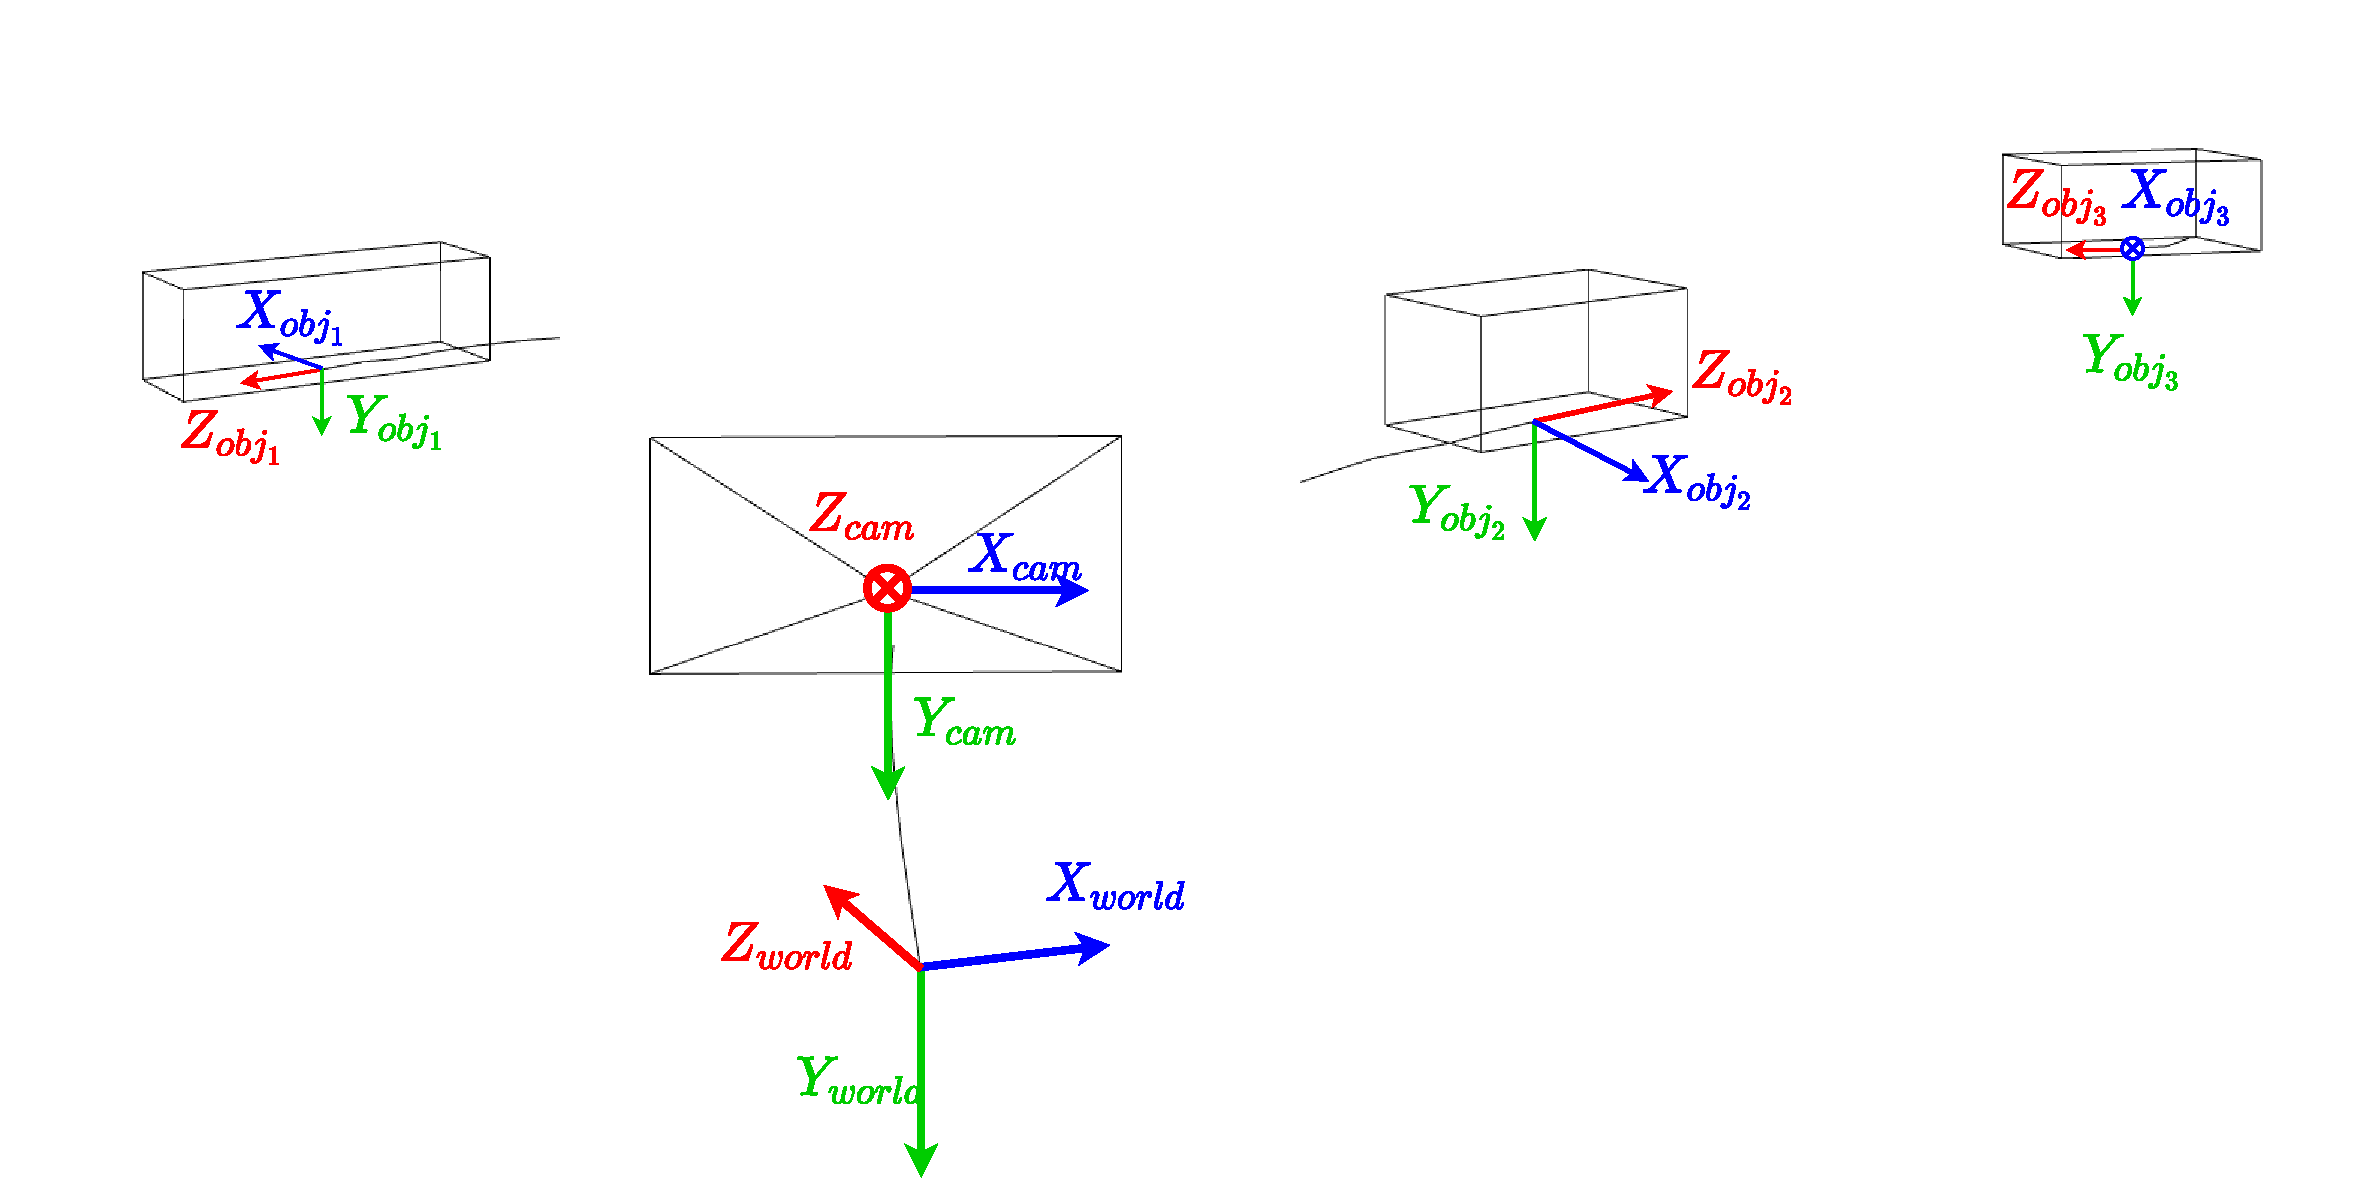
\includegraphics[width=.9\linewidth]{figures/cosys.pdf}
\caption{\label{fig:cosys}An illustration of the different coordinate systems/poses at a given time \(t\). The world frame is initialized to the first camera pose and kept fixed. The other poses are updated every frame.}
\end{figure}

As mentioned in \cref{modat}, a 3D object is typically expressed by an \gls{oobb}
This \gls{oobb} comprises the object location \({}^w\mathbf{t}\) in world coordinates, the object's dimensions (height, width, length) and its yaw (i.e., rotation around its vertical y-axis). 
We give a visualization of such an \gls{oobb} in \cref{fig:oobb}.
We estimate the \gls{oobb} for each time step. Connecting the object's locations over time forms a 3D trajectory.

\begin{figure}[htbp]
\centering
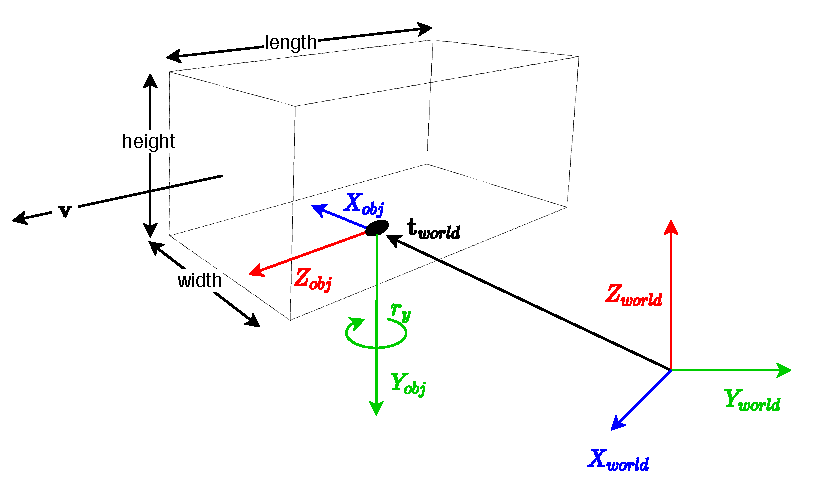
\includegraphics[width=.9\linewidth]{figures/oobb.pdf}
\caption{\label{fig:oobb}The \gls{oobb} typically describes objects for the 3D \gls{mot} task. Note that this state simplification does not allow a pitch rotation and hence assumes level roads.}
\end{figure}


\section{System Overview}
\label{sec:org13b094a}
   The proposed method for 3D \gls{mot}, termed \gls{bamot}, combines several techniques from related problems: 2D \gls{od} and tracking (see \cref{modat}), and visual SLAM (see \cref{slam}).
The suggested overarching system is a composition of the following functionalities:

\begin{samepage}
\begin{enumerate}
\item stereo multi-object detection
\item detection-track association
\item 3D object tracking
\end{enumerate}
\end{samepage}

The division of \gls{bamot} into these loosely-coupled subsystems allows easy interchangeability of all subsystems with updated procedures, e.g., an improved 2D object detector, a different method for associating tracks with detections, 
or other feature point extraction or matching techniques. The boundaries between the subsystems allow these types of changes and facilitate incremental development and improvements along any of these
three dimensions. A rough qualitative overview of the proposed system is given in \cref{fig:system-overview}.

Note that the sensors used as input to the system potentially create further inter-dependencies and requirements for the subsystems.

\begin{figure}[htbp]
\centering
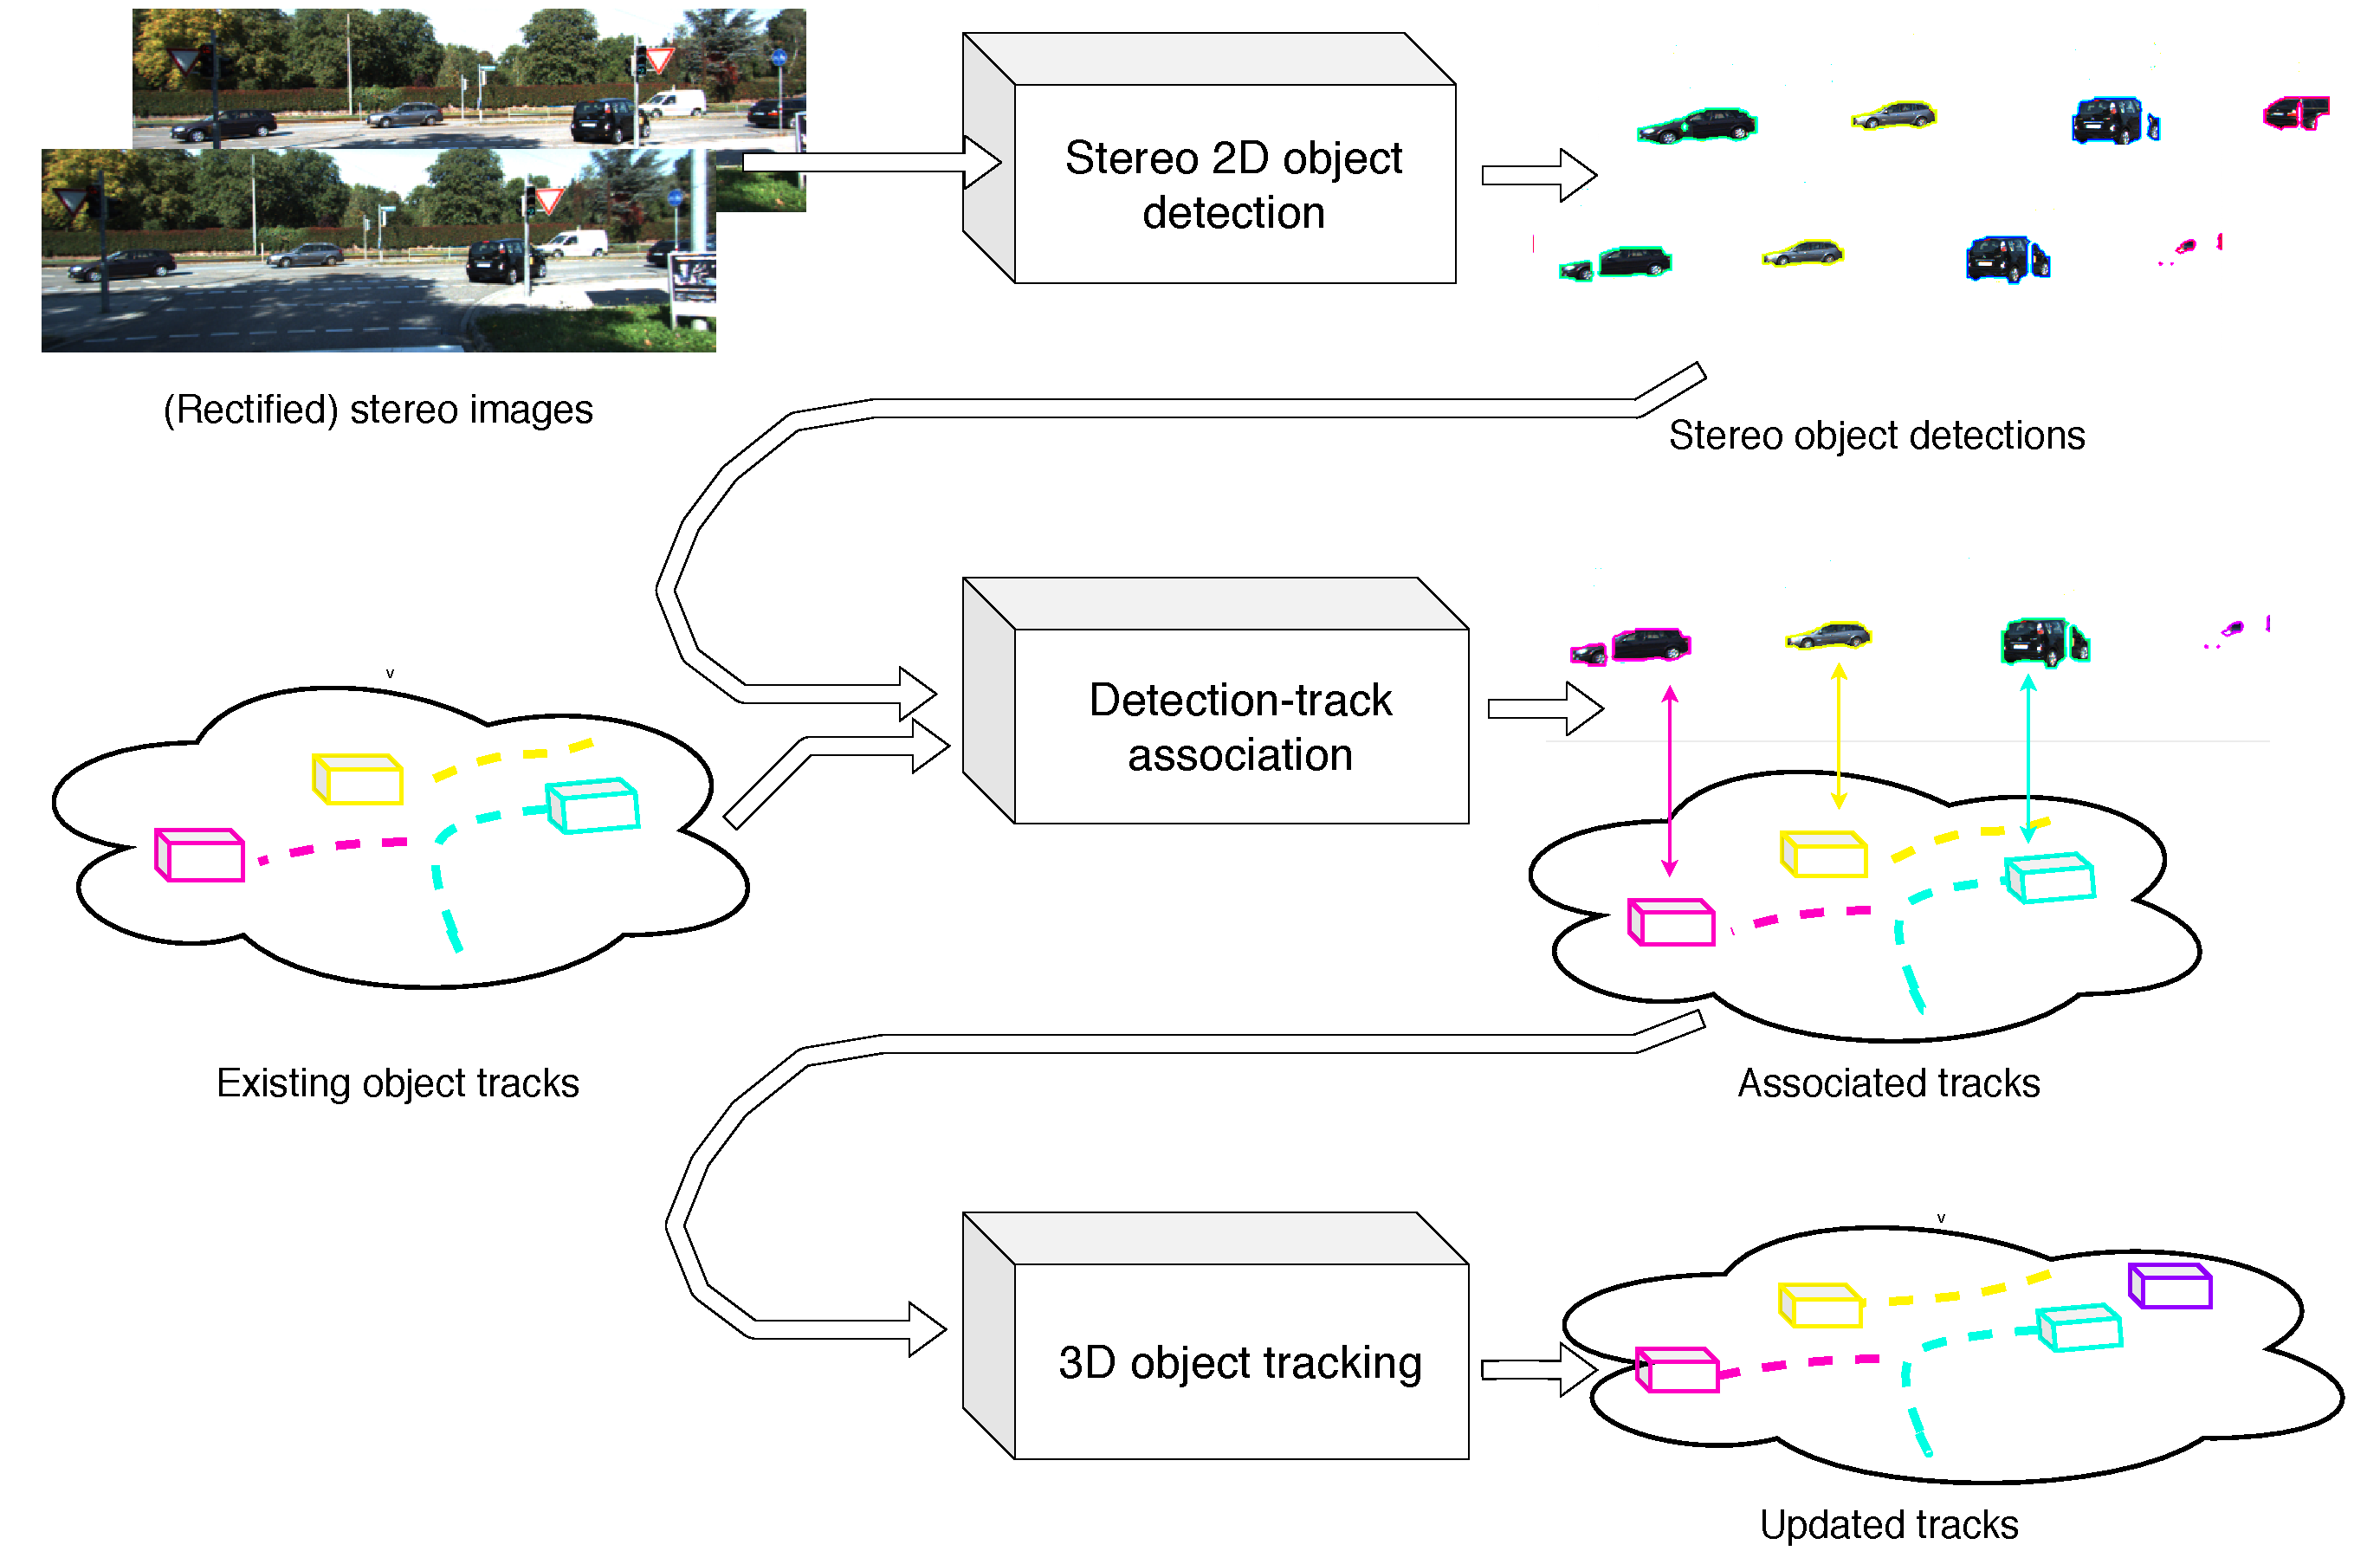
\includegraphics[width=0.9\textwidth]{figures/system-overview.pdf}
\caption{\label{fig:system-overview}A coarse sketch of BAMOT. The proposed process consists of three steps: 2D stereo object detection, detection-track association, and 3D object tracking.}
\end{figure}

\section{Sensors}
\label{sec:org186f36f}
    In this work, two stereo-calibrated RGB cameras are the sensory input in form of a stream of rectified images. 
This rectification is not principally necessary: 
one can also achieve 2D object detection, feature point extraction and matching, and stereo triangulation using non-rectified (but calibrated) cameras.
However, we evaluate this thesis on the popular KITTI dataset (see \cref{kitti-dataset}), which provides rectified images.
\section{Stereo 2D Multiple Object Detection \label{stereo-2d-mod}}
\label{sec:org5d5e62c}
    The first step in BAMOT is detecting objects from both stereo images, \(I_l\), and \(I_r\), in 2D and associating left and right object detections. The resulting detections are now 2D stereo object detections.
The object detector used in BAMOT is the deep-learning-based TrackR-CNN introduced in \Cite{voigtlaenderMOTSMultiObjectTracking2019} which extends MaskR-CNN \cite{heMaskRCNN2018} with association capabilities. 
This 2D tracker outputs pixel-wise segmentation masks and object classes per detection. 
Both left and right images pass through the detection network. The result is two collections of segmentation masks, \(M_l^i\) and \(M_r^j\), of sizes \(s_l\) and \(s_r\), respectively.

\begin{figure}[htbp]
\centering
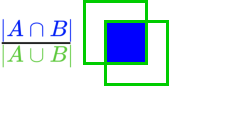
\includegraphics[width=0.25\textwidth]{figures/iou.pdf}
\caption{\label{fig:iou}The Jaccard Index comes from set theory, but one often uses it as a similarity measure in object detection and association tasks. In this context, it is more commonly known as the Intersection-Over-Union measure.}
\end{figure}

Since the left and right masks are in different image domains and there is no way to transform a mask from the left image onto the right image without any depth information,
a simple area-based similarity score such as the widely-used Jaccard Index \cite{jaccardDISTRIBUTIONFLORAALPINE1912} or, its more common name in \gls{cv} tasks, Intersection-over-Union (see \cref{fig:iou}),
will produce erroneous associations, especially with many neighboring objects (see \cref{fig:bad-2d-association} as a qualitative example).

Thus, we use an appearance-based heuristic in addition to the \gls{iou} score. 
Feature points (see \cref{feature-points}) encode appearance and we already use these in the subsequent track-detection association and 3D multi-object tracking steps. 
Hence, we exploit this redundancy by using such features in multiple parts of the system and caching results in between steps.
We compute the appearance score as follows: first, we detect ORB \cite{rubleeORBEfficientAlternative2011} features in both images. This results in two sets of feature points \(f_l\) and \(f_r\) with sizes \(n_l\) and \(n_r\), respectively. 
Next, we match these features as described in \cref{feature-points}. This then leads to to \(n_m\) stereo matches. 
Finally, the ``normalized'' matched features score \(\lambda_f\) is:

\begin{equation}
\label{eq:appearance-score}
\lambda_f = \frac{n_m}{\max(1, \min(n_l, n_r))} 
\end{equation}

This score is zero if there are no feature matches and maximized to 1 if at least one collection of features (left or right) is matched perfectly (unless there are zero matches in either the left or right image).
This score puts more weight on the number of matched features per object than on the number of matched features in total and allows to match objects that are occluded or truncated in one image but not (or less so) in the other. Putting more weight on the total number of matches would, for example, result in \cref{eq:appearance-score-alt}.
Note that as an additional measure, detections with different class predictions receive a score of 0.

\begin{equation}
\label{eq:appearance-score-alt}
\lambda_f = \frac{n_m}{\max(1, \max(n_l, n_r))} 
\end{equation}

Using the former equation vs. the latter empirically proved to result in superior associations. 
The resulting final score is in the range of \([0, 2]\):

\begin{equation}
\label{eq:final-score-2d-association}
\lambda = \lambda_f + IoU(M_l^i, M_r^j)~\text{with}~IoU(A, B) = \frac{|A \cap B|}{|A \cup B|}
\end{equation}

\begin{figure}[htbp]
\centering
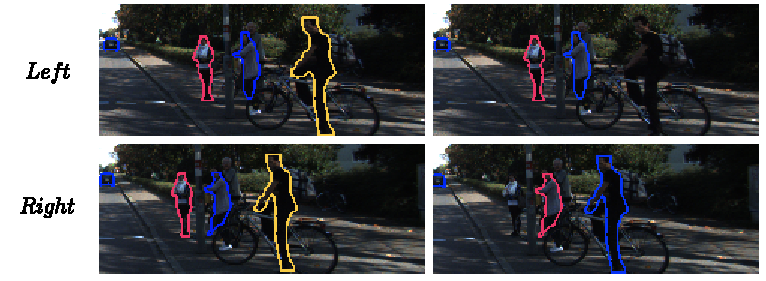
\includegraphics[width=.9\linewidth]{figures/bad-2d-association.pdf}
\caption{\label{fig:bad-2d-association}\emph{Left}: Left-right object association is done using the similarity measure from \cref{eq:final-score-2d-association}. \emph{Right}: Using only IoU as a similarity measure results in bad associations as areas from different image domains cannot be compared. Note that in this qualitative example unmatched detections that are ``extrapolated'' into the other image domain are left out for simplicity.}
\end{figure}

After association, there may still be unmatched detections in both the left and the right image. 
To keep these potentially correct detections, we ``transform'' the segmentation mask of an unmatched detection in the left or right image to the respective other image.
This transformation is simply a dilation of the mask followed by a removal of pixels that they are already part of a different detection.
The resulting set of masks are thus non-overlapping. 
The introduced system dilates the mask by a dynamic number of pixels. This amount is inversely proportional to the mask's size \(m_s\).
The notion behind this heuristic is that as the object becomes smaller, the likelihood of correctly ``hitting'' parts of the object in the other image becomes smaller
and vice versa. Setting the proportionality factor to 2\% of the image area \(A=h \cdot w\) works well empirically. 
Additionally, we set the dilation to be at least 1px and at most 5\% of the smaller image dimension \(d_s=\min(h, w)\). Again, we determined these values experimentally.
The resulting number of pixels \(p_d\) the system dialates mask is then:

\begin{equation}
\label{eq:dilate-px}
p_d = \min(\lfloor 0.05 \cdot d_s \rfloor, \max(1, \lfloor\frac{0.02 \cdot h \cdot w}{m_s}\rfloor)))
\end{equation}

If the dilated mask is empty (because other detections fully occlude it), the detection remains unmatched, and the system subsequently discards it.
A flow diagram of the 2D stereo object detection process is given in \cref{fig:flow-2d-detection}. 

\begin{figure}[htbp]
\centering
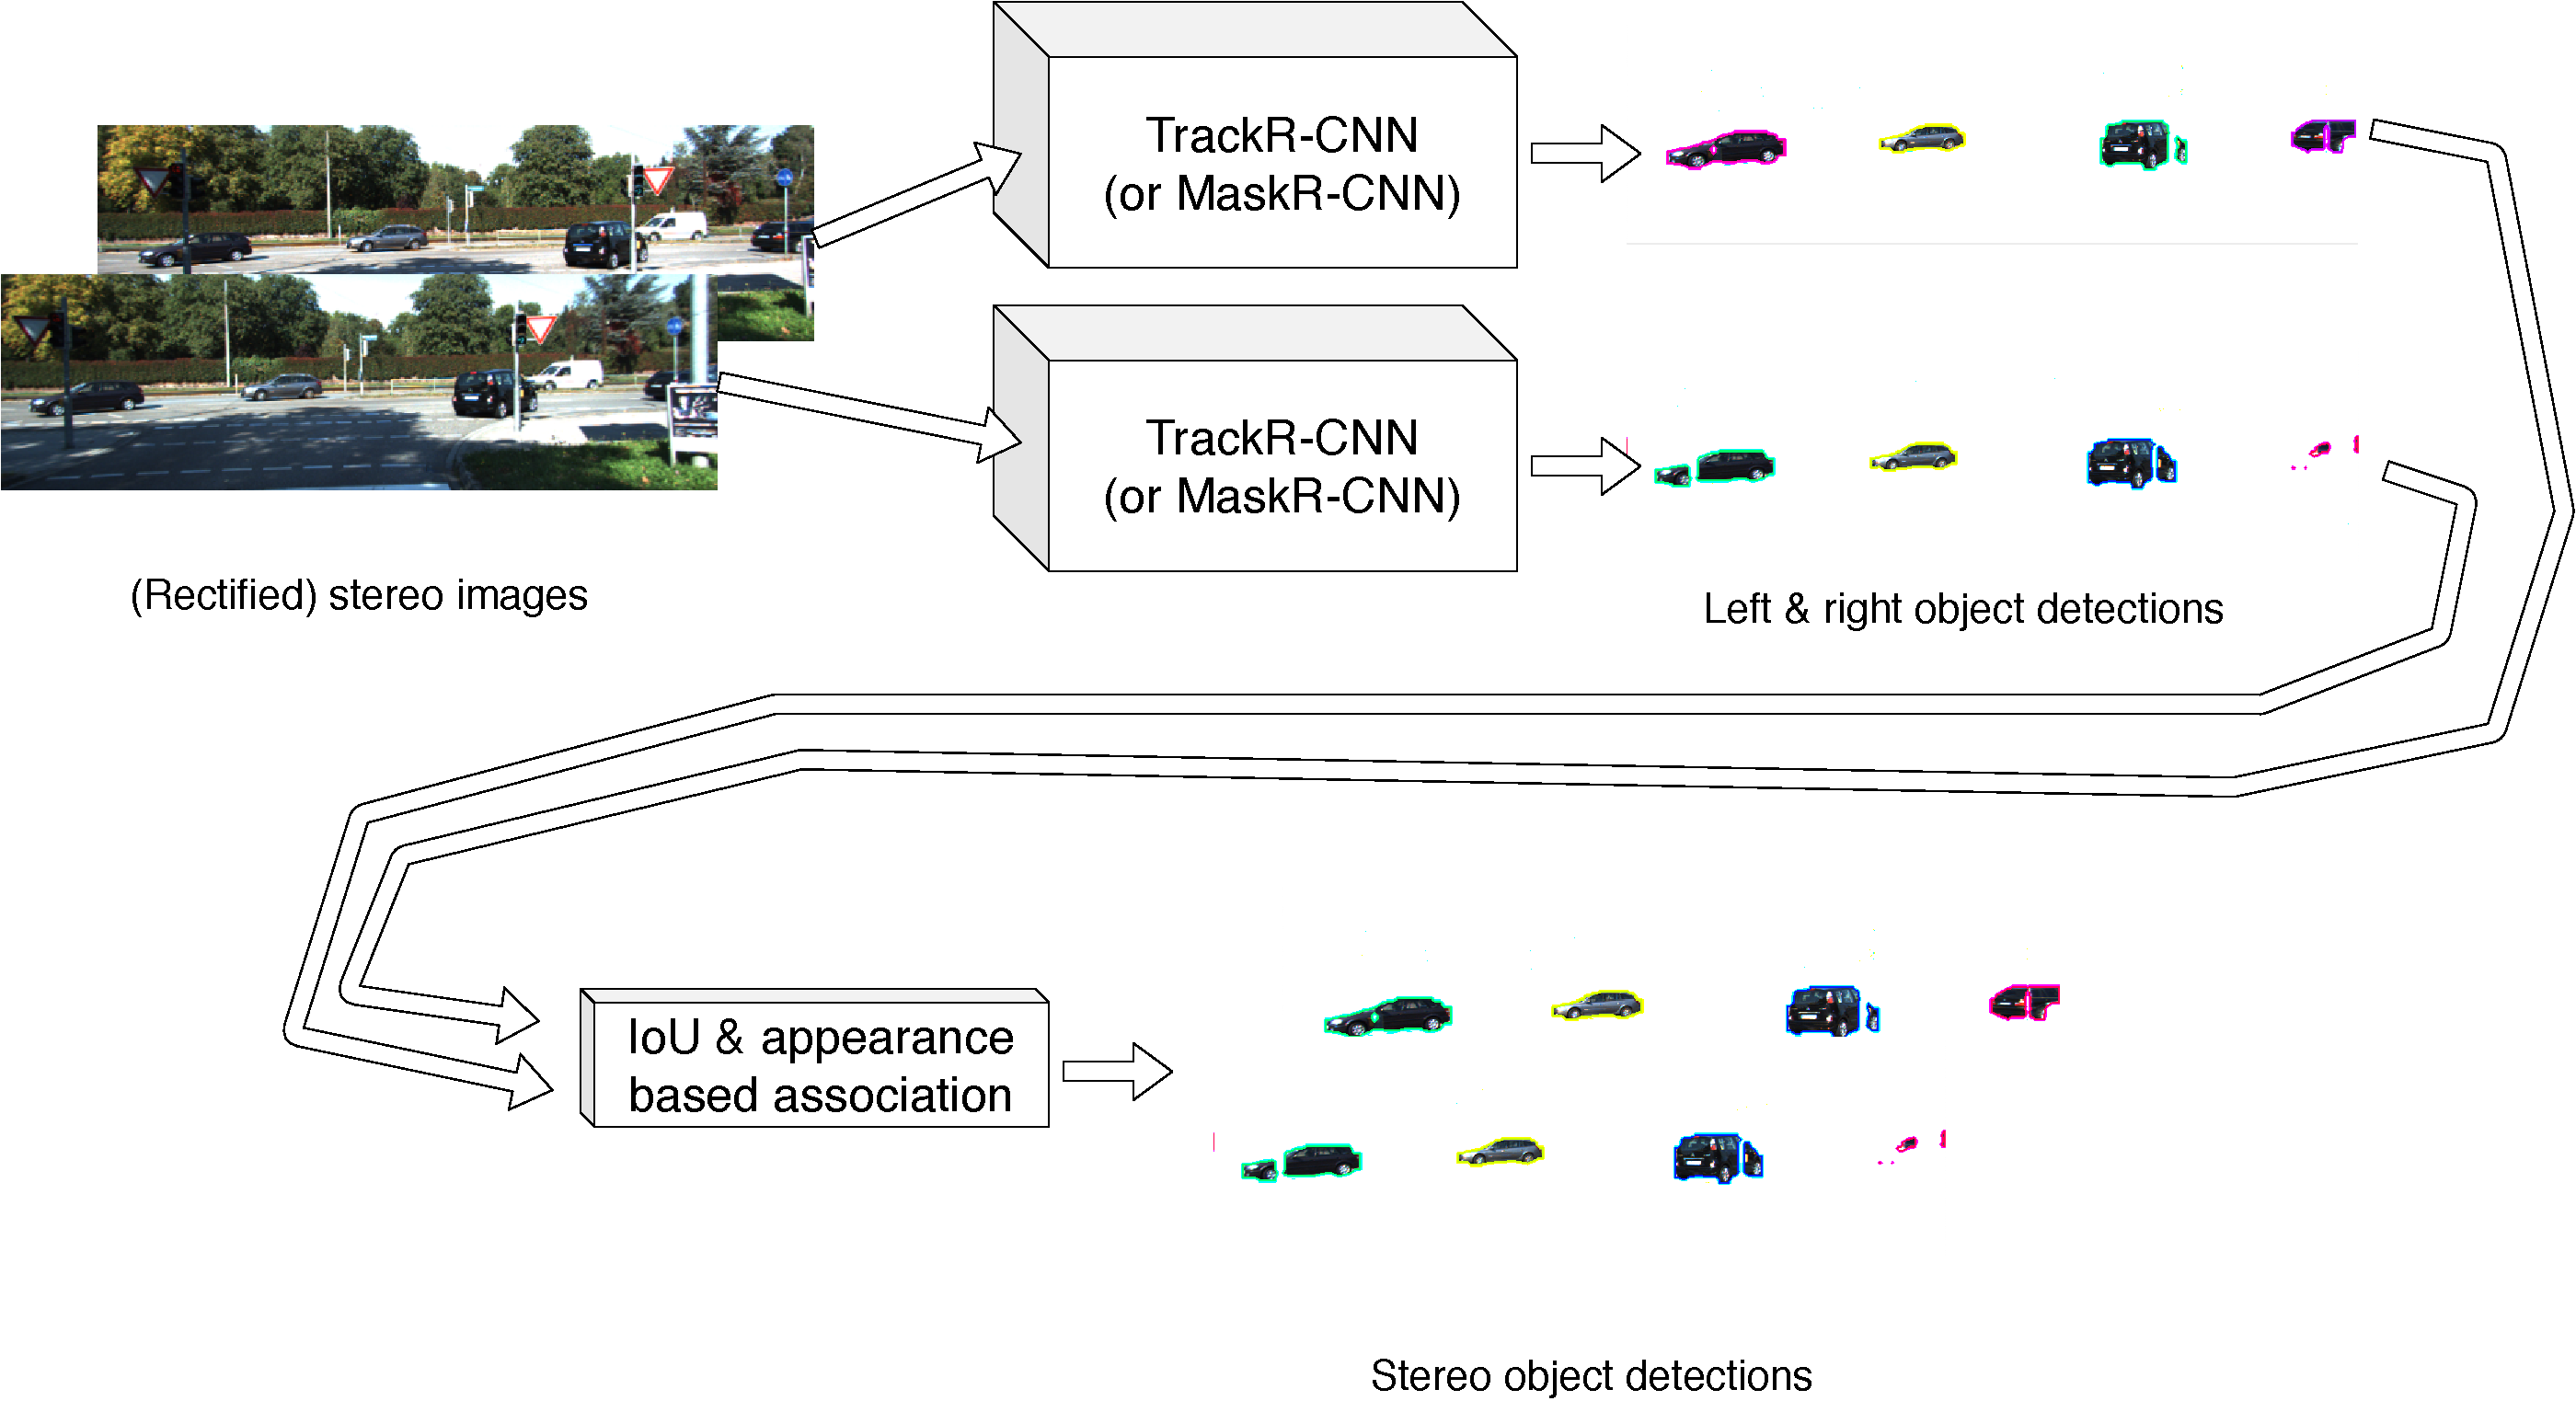
\includegraphics[width=.9\linewidth]{figures/flow-2d-detections.pdf}
\caption{\label{fig:flow-2d-detection}First, left and right images pass through a 2D object detector. Then the system associates the resulting detections between the two images using a similarity measure consisting of a proposed combination of the classical IoU and a ``normalized'' matched feature ratio score.}
\end{figure}

\section{Detection-Track Association \label{detection-track-assoc}}
\label{sec:orgc041b59}
   As the name suggests and as previously mentioned, the object detector we employ in \cref{stereo-2d-mod}, TrackR-CNN, is in fact a two-stage 2D multi-object tracker that extends the 2D multi-object detector MaskR-CNN.
In its first stage, TrackR-CNN detects segmentation masks and encodes the appearance of each object.
The association step of TrackR-CNN happens in the second-stage of the network. In this stage, the network learns to associate the encoded appearance vectors of the detected objects from the first stage.
For many cases, this works well; however, several scenarios exist where this process fails, e.g., for objects that look similar (resulting in false positives) or for those that change their subjective appearance resulting from a substantially different viewing angle (false negatives). 
Another error source is partial (or complete) occlusions and truncations and their effect on the encoded appearance.

Additionally, as the network learns this association, it adds another non-explainable component to possibly safety-critical applications (unlike, say, associations based on \gls{iou}). 
Fortunately, our proposed system has additional 3D information that it can utilize to supplement or altogether replace the learned associations from TrackR-CNN.
The proposed detection-track association consists of several consecutive association steps:

\begin{enumerate}
\item association based on the combination of appearance and 3D location
\item 3D corroborated 2D association (optional, only if the object detector is an object tracker such as TrackR-CNN)
\item association using only 3D location
\end{enumerate}

Note that the proposed system discards track-detection combinations for the first and second step where the track's object class does not match that of the detection. 
Additionally, we remove out-of-view tracks: track for which no landmarks can be projected to valid left image coordinates.

\subsection{Association via Combined Appearance \& Location \label{combined-assoc}}
\label{sec:org9fe6625}
    Tracking based either entirely on appearance or the location (both 2D and 3D) of objects is sub-optimal. Appearance changes or is non-unique (to a certain degree), projected 2D positions (e.g., masks or bounding boxes) lose
valuable depth information, and both 2D and 3D locations can become ambiguous when objects appear close to one another (especially at greater distances).
Therefore, combining these two similarity measures is desirable as it presumably leads to a more robust association less susceptible to either measure's shortcomings. 
One approach to a unified measure would be to calculate the similarity of appearance and location separately and then merge these two scores in some fashion.
However, this merging into a single similarity measure for an association is not straightforward and requires some underlying parameterized model. BAMOT uses such a scheme for 
stereo object association (see \cref{stereo-2d-mod}) in 2D which works sufficiently well in practice; however, in the case at hand, associations are not merely snapshot-based 
(i.e., objects only have to be matched between a single left and a single right image) but detections have to be robustly re-matched to tracks that have potentially become occluded for several frames 
(and conversely,  detections of new tracks should not wrongly be associated to existing tracks which have become occluded).
Hence, it is preferable to use a measure that incorporates appearance and 3D location ``out-of-the-box''. 

One such procedure is \gls{pnp} (see \cref{pnp}):
\gls{pnp} estimates a transformation given a set of 2D-3D correspondences. Typically (i.e., in \gls{vo} or \gls{slam}), the 3D points are landmarks in a static map, the 2D points are observations of these
points on an image plane of a camera, and the resulting transformation is the camera pose w.r.t. the static map.
In the proposed implementation, the 3D points are landmarks of an object w.r.t. that object's coordinate frame, and the resulting transformation is the object pose w.r.t. the fixed world frame.
The reasoning behind adopting \gls{pnp} (over, say point cloud alignment via 3D-3D correspondences using, e.g., \gls{icp} \cite{chenObjectModellingRegistration1992}) is that we already employ this procedure in the following 3D object tracking step.
See \cref{3d-ot} for a full description of the adjusted \gls{pnp} method. 
Hence, we can reuse the computed poses. 
\gls{pnp} uses appearance (feature points-landmark matches) and 3D information (object landmarks and the resulting pose \({}^{c}_{o}T_t \in \mathbb{R}^3\)). 
As mentioned above, we cache the feature points per object detection from the previous 2D stereo object detection step. 
We match these with the landmarks of each existing track.
The following Section on 3D object tracking (\cref{3d-ot}) explains our features-landmark matching method.

\gls{pnp} doesn't directly result in a similarity measure that the system can employ for associations. 
However, it does output a normalized ratio of success: the inlier ratio \(\lambda_i=\frac{n_i}{n}\) from the underlying \gls{ransac} scheme (see \cref{ransac}) where \(n_i\) is the number of inliers, and \(n\) is the total number of points used in the estimation (i.e., the number of 2D-3D matches). 
Nonetheless, we cannot use the inlier ratio directly as a measure of similarity: take, as a concrete example, an object-track combination with five 2D-3D correspondences and an inlier ratio of 1.0 vs. an object-track 
combination with 100 2D-3D matches and an inlier ratio of 0.99.
Adding a third object-track combination with 200 2D-3D correspondences and an inlier ratio of 0.5 illustrates that using the raw number of inliers also doesn't work as a proxy for similarity.
Thus, we need to normalize the number of inliers in some other way. 
Two factors limit the maximum number of inliers \(n_{max}\), or, equivalently, the maximum number of 2D-3D correspondences. 
First, the number of landmarks \(n_l\) of an object, and second, the number of features \(n_f\) in a detection. Consequently, \(n_{max} = \min(n_l, n_f)\). 
This allows for both occluded objects (\(n_l\) will be high, but \(n_f\) small) and objects 
coming into view (\(n_l\) will be low, but \(n_f\) high).
Thus, the resulting similarity measure is:
\begin{equation}
\lambda = \frac{n_i}{n_{max}} 
\end{equation}
If the pose estimation fails, we set the measure to 0.

As an additional criterion to check the success of the pose estimation, our system assesses the validity of the translational component.
We consider a pose estimate valid if the relative object translation w.r.t. the previous pose at time \(t-1\) is within a certain distance \(d_{max}\):
\begin{equation}
|\mathbf{t}_{rel}| <= d_{max} ~ \text{with} ~ ({}^{c}_{o}T_t)^{-1}{}^{c}_{o}T_{t-1}={}^{o_t}_{o_{t-1}}T = \begin{bmatrix}\mathbf{R}_{rel} & \mathbf{t}_{rel} \\ \mathbf{0}^T & 1 \end{bmatrix}
\end{equation}

If this ``motion'' is deemed invalid, we set the similarity measure to 0.

Three parameters influence the heuristical function behind \(d_{max}\): 

\begin{enumerate}
\item the object type (i.e., a pedestrian is slower than a car)
\item the distance of the object from the camera \(d_c\) (i.e., the accuracy of pose estimation decreases with distance to the camera)
\item the number of consecutive frames that BAMOT was not able to associate a track to a detection (see the following \cref{3d-ot})
\end{enumerate}

Each object-type \(i\) has a fixed maximum expected speed of \(v_i\). 
This speed multiplied by the frame rate \(T\) gives a baseline maximum translation \(\tilde{d}_{max} = T \cdot v_i\).
This baseline defines the radius of a sphere around the previous location that an object is expected to maximally travel between two frames.
We multiply this radius by a factor which conceptually acts as a measure of uncertainty (as determined by parameters two and three of the preceding listing) of the previous location, 
e.g., if the ambiguity of the last position is high, this factor is greater than 1.
The uncertainty arising from the distance to the camera \(d_c\) stems from fewer features detected on a smaller object (hence the pose estimation can use fewer 2D-3D associations as well). Additionally, 
triangulation accuracy decreases with distance. The authors of ORB-SLAM \cite{mur-artalORBSLAMVersatileAccurate2015a,mur-artalORBSLAM2OpenSourceSLAM2017} empirically determined that up until a distance of \textasciitilde{}20 times the baseline \(b\) of the stereo cameras (see \cref{epipolar-geometry})
triangulation is accurate. For this reason the distance component \(f_d\) is as given in \cref{eq:dist-factor}. It is 1 for distances beneath the threshold \(d_b = 20 \cdot b\) and the distance divided by \(d_b\) 
for greater distances. 

\begin{equation}
\label{eq:dist-factor}
f_d(c_d) = 
\begin{cases}
1{}\text{, if }{}d_c < d_b \\
\frac{d_c}{d_b}{}\text{, else}
\end{cases}
\end{equation}

The third parameter, the number of frames \(n_{bad}\) for which no 2D stereo detections exist, is another source of uncertainty of the object location. 
BAMOT incorporates this into the final multiplicative factor by multiplying \(n_{bad}\) by a factor \(f_{bad}\) and adding one to the fraction (s.t. the multiplier doesn't become zero when the object's location uncertainty is due to its distance from the camera and not due to missing detections).
Additionally, the multiplicative factor is limited by a constant \(f_{max}\) to restrict the possible locations and avoid false-positive associations. This cutoff essentially gives an upper bound to the maximally
acceptable uncertainty of an object's location when associating it to detections.
Overall, the resulting allowed distance is:

\begin{equation}
\label{eq:max-dist}
d_{max} = f \cdot \tilde{d}_{max} = \min(f_{max}, f_d(c_d) \cdot (f_{bad} \cdot n_{bad} + 1)) \cdot T \cdot v_i
\end{equation}

A complete flow diagram of this process is presented in \cref{fig:pnp-assoc-flow}.

\begin{figure}[htbp]
\centering
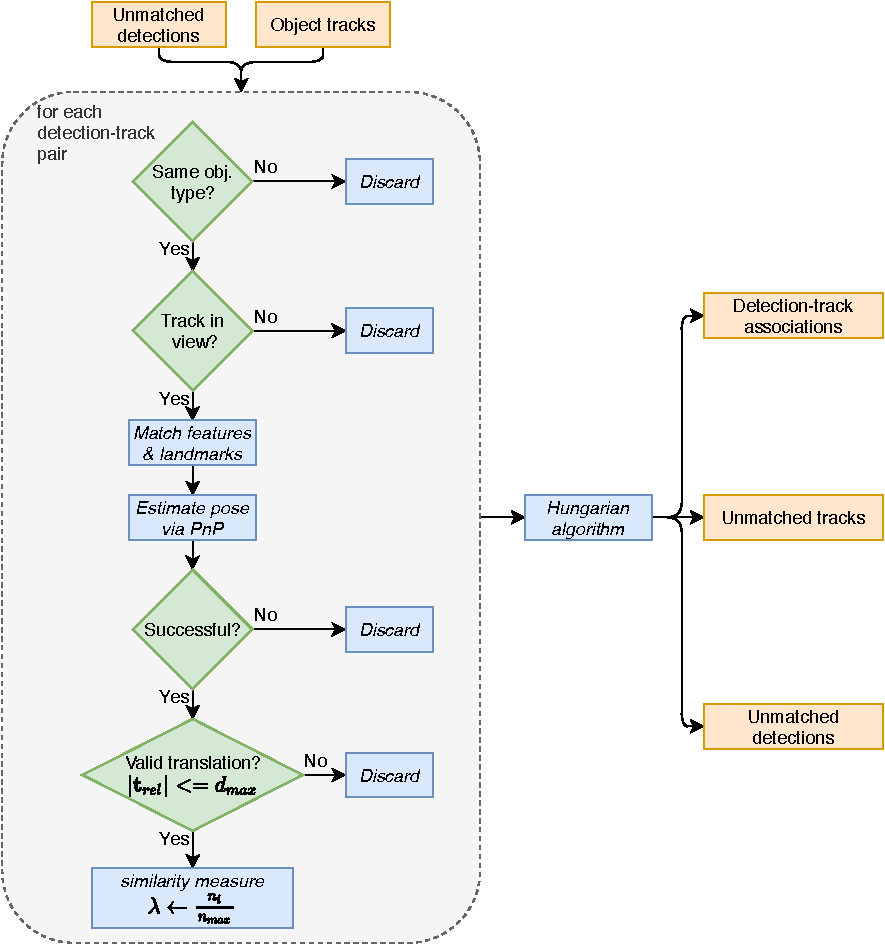
\includegraphics[width=.9\linewidth]{figures/match_detections_tracks_pnp.pdf}
\caption{\label{fig:pnp-assoc-flow}A flowchart of the detection-track association step based on PnP as described in \cref{combined-assoc}.}
\end{figure}



\subsection{3D Corroborated 2D Assocations}
\label{sec:org376927d}
    This next step is employed when the object detector is, in fact, a 2D object tracker such as TrackR-CNN. 
The idea behind this association step is to supplement the given 2D information (by the 2D tracker) with the available 3D information. 
We achieve this merging by corroborating (or discarding) 2D associations with the 3D location of a given detection and the associated object track as follows:
First, for every stereo detection, our system uses the stereo feature matches from the stereo detection association step (see \cref{stereo-2d-mod}) to localize the object in 3D space.
The proposed system accomplishes this localization by triangulating each stereo feature (see \cref{triangulation}) to compute a point cloud for a given detection. 
If we cannot successfully triangulate any points (and, hence, have no 3D information), the 2D association is discarded. 
Otherwise, the median point of the resulting point cloud is the location estimate. 
The median is more robust to outliers s.t. the accuracy of the resulting location will not suffer from few badly triangulated (because badly matched) features.
We then check whether the relative translation between the current location \(\mathbf{t}_0\) and the estimated location \(\mathbf{t}_{-1}\) from the previous frame (see \cref{3d-ot}) is valid:
\begin{equation}
|\mathbf{t}_{rel}| = |\mathbf{t} - \mathbf{t}_{-1}| \leq d_{max}
\end{equation}

The preceding association step does an equivalent validation when it verifies the PnP-estimated pose's resulting translational component. 
If the translation is acceptable, we adopt the association emanating from the 2D tracker.
Lastly, if the 2D tracker initializes a new track, we respect this, and the system creates a new track. 
Again, we provide a flowchart of this process in \cref{fig:2d-corroborated-flow}. 

\begin{figure}[htbp]
\centering
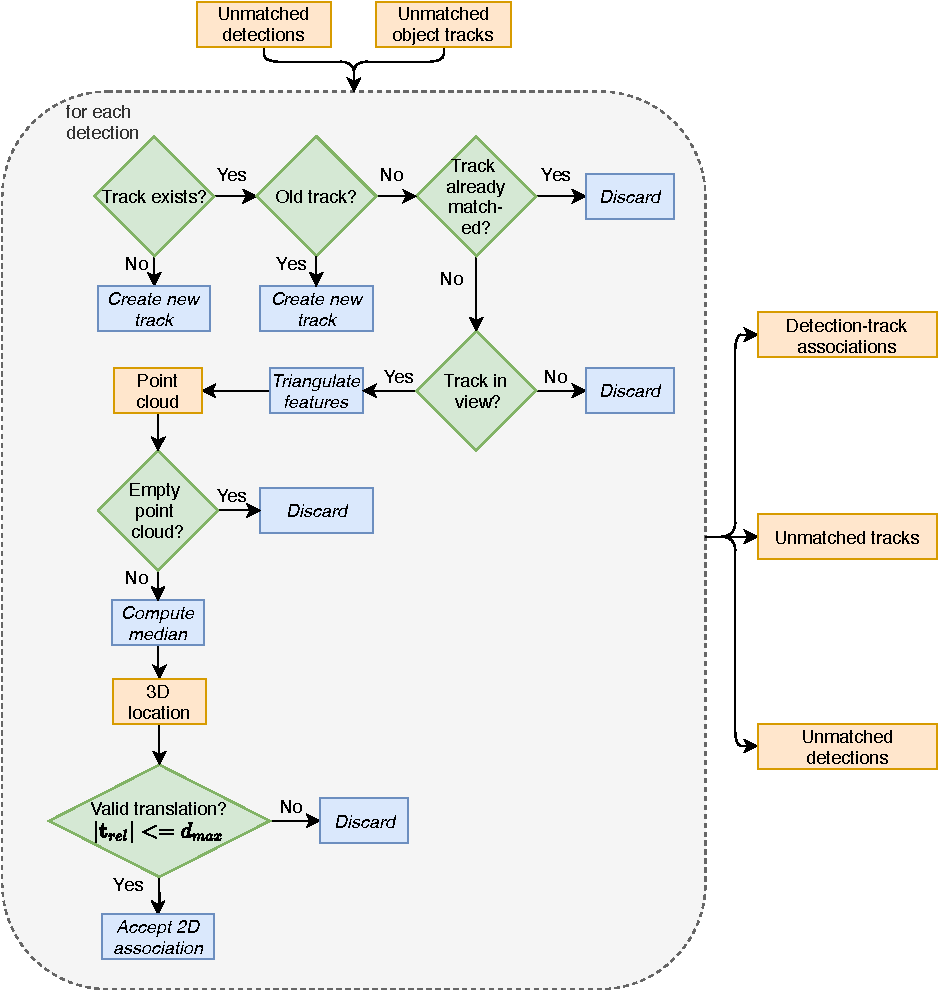
\includegraphics[width=.9\linewidth]{figures/match_detections_tracks_2d.pdf}
\caption{\label{fig:2d-corroborated-flow}If the 2D object detector is a tracker (such as TrackR-CNN), the second step in the association method corroborates the 2D associations using 3D information. This flow diagram depicts this procedure.}
\end{figure}

\subsection{Association via 3D location}
\label{sec:org14836d6}
    The association pipeline's final step is to associate tracks and detections using only their respective locations in 3D space.
For each detection-track combination, the similarity measure used by the Hungarian algorithm (see \cref{object-tracking}) is the 3D distance between the estimated track and the detection.
We estimate the location for a given detection via its point cloud's median point. As in the previous step, we create the point cloud by triangulating the stereo matches.
In line with the preceding stages, the distance between a detection-track pair needs to fall within a threshold \(d_{max}\) (see \cref{eq:max-dist}) to be considered a successful association. 
\cref{fig:3d-assoc-flow} shows an overview of this final phase.

\begin{figure}[htbp]
\centering
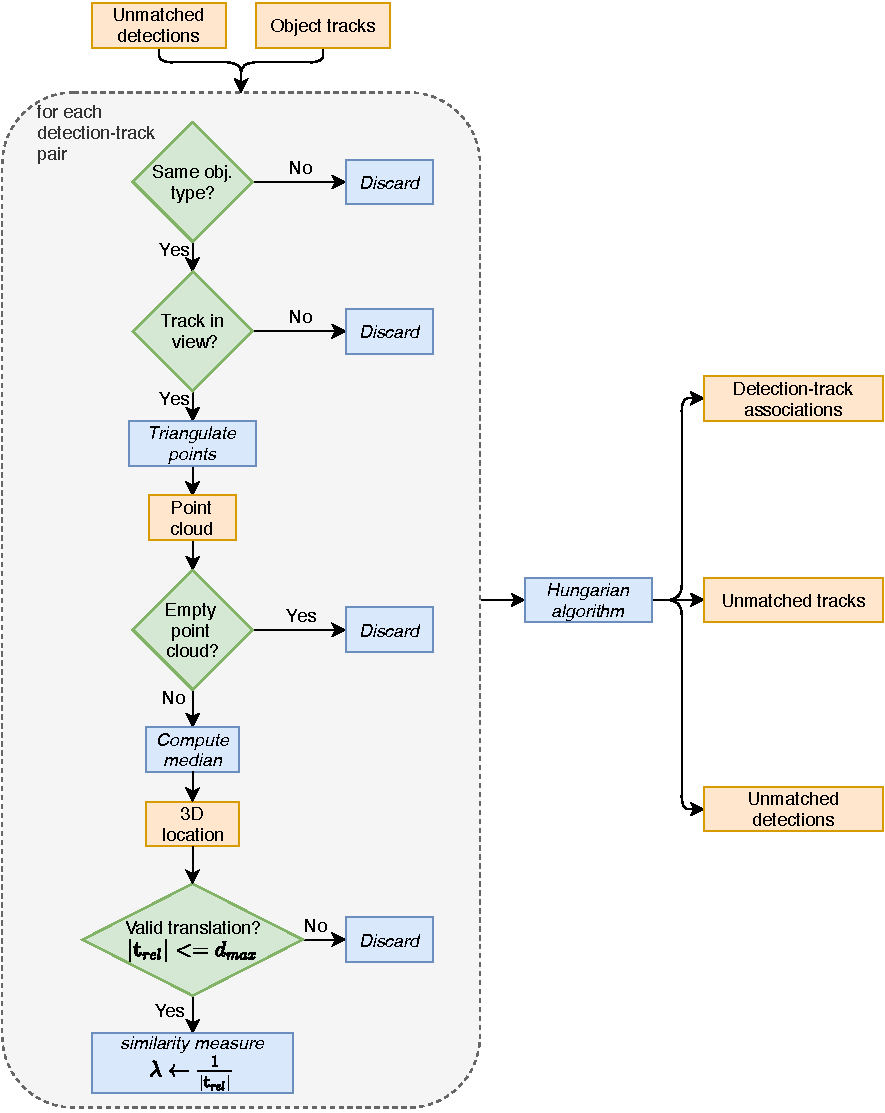
\includegraphics[width=.9\linewidth]{figures/match_detections_tracks_3d.pdf}
\caption{\label{fig:3d-assoc-flow}The final stage in the association pipeline: detections and tracks are associated solely by their similarity in 3D space. Note that BAMOT already performs some of these steps (e.g., creating point clouds) in a previous stage. However, the steps are shown here for completeness.}
\end{figure}

BAMOT creates new tracks from detections that remain unmatched after this three-step association pipeline.

\section{3D Object Tracking \label{3d-ot}}
\label{sec:org2b8c4a1}
   The proposed 3D object tracking amounts to object-level \gls{slam} with modifications rooted in a priori knowledge of the object types' geometry and dynamics.
Landmarks of a given object are defined w.r.t. its coordinate system, i.e., its current pose. Every landmark can have multiple observations, i.e., 2D feature points matched to this landmark. 
For each frame, we estimate an object's pose w.r.t. the world frame.
Initially (i.e., when BAMOT initializes an object track), the object pose coincides with the current camera pose. 
Additionally, each object has a location associated with it.
As in the association pipeline, an object's location is its median landmark. This location is always given in the current frame at time \(t\) w.r.t. the world coordinate frame.
The previous locations make up an object's trajectory and we use it to compute an object's \gls{oobb}. 

Three track categories exist after associating 2D detections to existing tracks: unmatched tracks, matched tracks, and new tracks.

\subsection{Extrapolating Motion For Unmatched Tracks}
\label{sec:org9bb640c}
    For unmatched tracks, i.e., tracks with no corresponding 2D detection, BAMOT extrapolates the locations. This extrapolation rests on a constant (local) motion assumption across a span of \(n_{rel}\) frames.
That is, for a track with \(n_p\) poses we take the previous poses \({}^{w}_{o}\mathbf{T}_{t-1}\) and \({}^{w}_{o}\mathbf{T}_{t_0}\) from time \(t - 1\) and \(t_0 = t - \min(n_{rel}, n_p)\), and then determine the average relative translation between these:
\begin{equation}
\overline{\mathbf{t}}_{rel} = \frac{\mathbf{t}_{t-1} - \mathbf{t}_{t_0}}{\min(n_{rel}, n_p)}
\end{equation}
We then compute the next pose \({}^{w}_{o}T_t\) by keeping the rotational component \({}^{w}_{o}\mathbf{R}_{t-1}\) equivalent and adding \(\overline{\mathbf{t}}_{rel}\) 
to the previous translational vector \(\mathbf{t}_{t-1}\):
\begin{equation}
{}^{w}_{o}\mathbf{T}_t = \begin{pmatrix}{}^{w}_{o}\mathbf{R}_{t-1} & (\mathbf{t}_{t-1} + \overline{\mathbf{t}}_{rel}) \\ \mathbf{0}^T & 1 \end{pmatrix}
\end{equation}
For tracks with only a single pose we have no translational estimate so the extrapolated pose is kept equivalent to the previous pose (\({}^{w}_{o}\mathbf{T}_t={}^{w}_{o}\mathbf{T}_{t-1}\)).
Additionally, we consider these unmatched tracks as poorly tracked and record the number of consecutively poorly tracked frames per object. If this counter goes above a certain threshold \(t_{bad}\), 
we consider the track inactive, remove it from future association steps, and do not record its \gls{oobb}.

\subsection{Object Pose Estimation}
\label{sec:org8e7e12a}
    The tracking procedure is broadly equivalent for new and matched tracks and we henceforth describe it for a single track.
First, the system resets the badly tracked frames counter to zero. Then it estimates the current pose. 
For matched tracks, the pose extrapolation procedure explained in \cref{detection-track-assoc} is the initial pose guess. 
We then refine this guess using \gls{pnp} estimation in a \gls{ransac} scheme (see \cref{pnp} and \cref{ransac}, respectively). 
However, we reframe the typical PnP problem as we are interested in the object and not in the camera motion.
Note that our system assumes the camera pose \({}^{w}_{c}\mathbf{T}_t\) to be given. 
In addition to the camera pose, we require the feature-landmark matches for this. These are available from the preceding detection-track association step (see \cref{detection-track-assoc}).
Also, notice that as the system performs four-point PnP (and not, e.g., the underdetermined P3P \cite{xiao-shangaoCompleteSolutionClassification2003}), our initial pose guess remains unchanged if there are fewer than four matches.
Usually, PnP estimates the camera pose w.r.t. landmarks of a static map. However, in this application, each object is its own static map, i.e., landmarks are in object coordinates. 
The poses that BA optimizes are the relative poses between the camera and the object. 
\cref{eq:pnp-bamot} gives the corresponding optimization objective of minimizing the reprojection loss function where \(\mathbf{p}_i\) and \({}^o\mathbf{P}_i\) are a 2D feature-object landmark combination.

\begin{equation}
\label{eq:pnp-bamot}
\min_{{}^c_o\mathbf{T}} \sum_i^n||\mathbf{p}_i - \pi({}^c_o\mathbf{T}{}^o\mathbf{P}_i)||_2^2
\end{equation}

If PnP successfully estimates a transformation, and the inlier ratio is greater than \(\lambda_{pnp}\), the system re-runs the procedure on the entire inlier set from the initial RANSAC optimization. 
Additionally, as in the first stage of the detection-track association procedure (see \cref{detection-track-assoc}), the translational component of the optimized pose is verified to be
less than \(d_{max}\) from \cref{eq:max-dist}. If the optimization is unsuccessful, has an inlier ratio below \(\lambda_{pnp}\), or the relative translation is too great, the initial guess (extrapolated pose) remains unchanged.

\subsection{Adding Landmarks and Observations \label{adding-lms-and-obs}}
\label{sec:orgc423021}
    We utilize stereo matches (see \cref{stereo-2d-mod}) and interest point-landmark matches (see \cref{detection-track-assoc}) to create new landmarks of an object and add observations of existing landmarks, respectively.
As explained in \cref{feature-points}, we require a descriptor for each landmark to perform descriptor matching between landmarks and (left) features. 
Our descriptor calculation for a landmark with \(n\) observations is inspired by ORB-SLAM \cite{mur-artalORBSLAMVersatileAccurate2015a,mur-artalORBSLAM2OpenSourceSLAM2017}: 
for each observation, we compute the distance of its descriptor to all other observations. Then, we determine the median of those distances per observation. Finally, 
we choose the observation's descriptor with the smallest median distance to all other observations as the landmark's representative descriptor. 
Unlike ORB-SLAM, there is no concept of ``keyframes'': BAMOT considers all frames for a given track. Consequently, landmarks may have many more observations than in a 
SLAM setting. Since the descriptor computation mentioned above has a runtime of \(O(n^2)\), the proposed system limits the number of descriptors used for comparison \(\tilde{n}\) to \(n_{max}\).
We sample the \(\tilde{n} \leq n_{max}\) descriptors uniformly from all available \(n\) observations.
Once (left) features have been matched to landmarks, we can add the features as observations. 
However, these features must fulfill two criteria: first, when transforming the matched object landmark to the current camera pose,
the point must not be behind the camera, and, second, its distance must not exceed a given threshold \(d_{max}^c\).
The system adds a stereo observation of the landmark if there exist a corresponding right feature point (i.e., the feature is also a stereo match) 
and if the left-right feature correspondence does not violate the epipolar constraint (as detailed in \cref{epipolar-geometry}).

After the preceding step, the system triangulates new landmarks (see \cref{triangulation}) from stereo matches (feature-feature matches from the left and right camera frames) 
that it did not yet add as observations to existing landmarks in the preceding step. 
Several conditions must hold for these newly created landmarks to be valid as well: they need to fulfill the epipolar constraint, the triangulated point must not lie behind the cameras, and finally, the distance of the point to the cameras may not exceed the threshold of \(d_{max}^c\). 
\cref{fig:add-lm-and-obs} shows the process of adding observations and landmarks.

\begin{figure}[htbp]
\centering
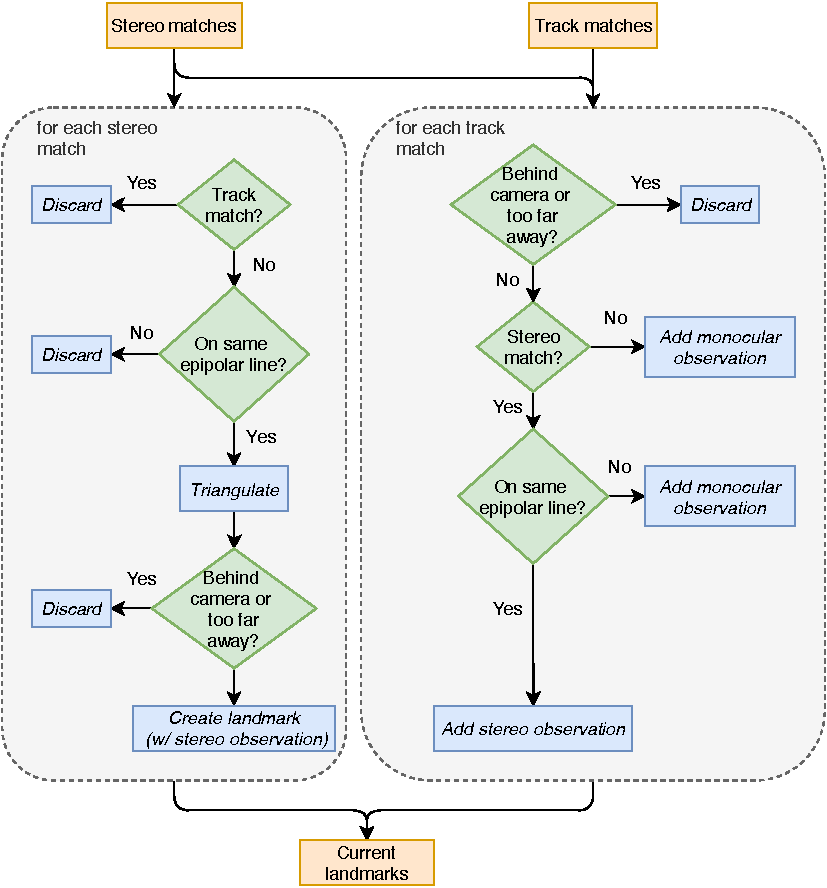
\includegraphics[width=.9\linewidth]{figures/add-lm-and-obs-flow.pdf}
\caption{\label{fig:add-lm-and-obs}The qualitative process of adding new observations to existing landmarks from feature matches between the left camera and landmarks and creating new landmarks from matches between the left and right camera frames. \cref{adding-lms-and-obs} explains the procedure in detail.}
\end{figure}


The set of newly created landmarks and observed landmarks, termed the current landmarks, are then used to remove stale landmarks in the following manner:
first, the center of the current landmarks is their median. 
Then, we mark all landmarks that are further from this center than an object-specific threshold as invalid and consequently delete them.
This object-specific threshold is the maximum expected object dimension for a given type (e.g., the length for cars and height for pedestrians).
Such a threshold ensures that even if the current landmarks are at the very edge of an object, the process does not remove existing landmarks at the object's opposing edge. 
This thresholding-based culling process proves to be a simple and powerful way to remove outlier landmarks based on known object dimensions. 
This is a deviation from regular SLAM systems as they do not have such geometric knowledge of the static map a priori.

As mentioned above, we set the object's initial pose to the current camera pose. 
However, once the object contains landmarks, we translate the coordinate system, so its origin lies at the median of the object's point cloud. 
This translation is necessary to limit the effect of camera rotation on motion estimates for far away objects. 
Finally, if the system did not create more than \(l_{min}\) landmarks, it discards the newly created track. 
This conservative track creation ensures more robust initialization at the potential cost of later than necessary initialization. 

\subsection{Object-level Bundle Adjustment \label{object-lvl-ba}}
\label{sec:org160d92d}
The classical SLAM problem consists of simultaneously finding the world positions of a collection of landmarks and the world poses of a set of camera poses where each pose observes some subset of the landmarks. One approach to solve this problem is through Bundle Adjustment (see \cref{slam}), a graph-based solution.

In the proposed system, each object \(k\) has \(n_k\) landmarks that are fixed w.r.t. the object's coordinate frame under the rigidity assumption.
Also, each object has \(t_k\) pose estimates w.r.t. the fixed world frame.
In order to simultaneously optimize the landmark positions and the object poses, we need to make some mathematical adjustments s.t. the problem can be solved via Bundle Adjustment.
Since the pose of the camera at time \(t\) is given as \({}^{w}_{c}\mathbf{T}_t\), estimating the relative pose between the camera and the object \(k\) at time \(t\) \({}^{o_k}_{c}\mathbf{T}_t\) results in the desired pose: 
\begin{equation}
{}^{w}_{o_k}\mathbf{T}_t = {}^{w}_{c}\mathbf{T}_t ({}^{o_k}_{c}\mathbf{T}_t)^{-1}
\end{equation}
Thus, we introduce a Bundle Adjustment scheme where both landmarks and camera poses are optimized w.r.t. the object frame. 
Since the camera poses w.r.t. the world frame are known, the system can deduce the needed object poses and landmarks w.r.t. the world frame.
\cref{eq:ba-bamot} displays the adjusted objective function for a single object \(k\) with \(n\) landmarks tracked over \(t\) frames with known camera poses over these frames. 
Note that \(\pi(.)\) is the known projection function, \(\mathbf{p}_{t}^{n}\) is the observed feature point for the landmark \(n\) at frame \(t\), and \(\rho(.)\) is the robust Huber kernel \cite{huberRobustEstimationLocation1964}. 
The Huber kernel limits outliers' influence: their residual is linear instead of quadratic.
The set of all landmarks is \(\mathbf{P}\) and the set of all object poses is \({}^o_c\mathbf{T}\).

\begin{equation}
\label{eq:ba-bamot}
    {}^{o}_{c}\mathbf{T}^*, \mathbf{P}^* = \min \sum_{n, t}\rho(||\mathbf{p}_{t}^{n} - \pi({}^{o}_{c}\mathbf{T}_{t}{}^{o}\mathbf{P}_{n})||^2)
\end{equation}

We further adjust this objective function via the addition of an error term that penalizes non-smooth trajectories. 
The idea is that objects are expected to have constant velocity, at least locally, and further that adding this requirement has a positive regularizing effect on the optimization problem. 
We express this constant motion requirement as follows: 
for three poses at times \(t\), \(t-1\), and \(t-2\), the relative object motion from \(t-2\) to \(t-1\) and from \(t-1\) to \(t\) must be identical.
The equality from \cref{eq:const-motion} shows that the necessary poses are \({}^{o}_{c}\mathbf{T}_{\tilde{t}}\) and \({}^{w}_{c}\mathbf{T}_{\tilde{t}}\) for \(\tilde{t} \in \{t-2, t-1, t\}\).
\({}^{o}_{c}\mathbf{T}_{\tilde{t}}\) are the poses that the \gls{ba} procedure optimizes and \({}^{w}_{c}\mathbf{T}_{\tilde{t}}\) are the known camera poses that we use as constants in the graph-optimization.

\begin{equation}
\label{eq:const-motion}
\begin{gathered}
{}^{o^{t-1}}_{o^{t-2}}\mathbf{T} = {}^{o^{t}}_{o^{t-1}}\mathbf{T} \\
{}^{o}_{w}\mathbf{T}_{t-1}({}^{o}_{w}\mathbf{T}_{t-2})^{-1} = {}^{o}_{w}\mathbf{T}_{t}({}^{o}_{w}\mathbf{T}_{t-1})^{-1} \\
{}^{o}_{c}\mathbf{T}_{t-1}({}^{w}_{c}\mathbf{T}_{t-1})^{-1}({}^{o}_{c}\mathbf{T}_{t-2}({}^{w}_{c}\mathbf{T}_{t-2})^{-1})^{-1} = 
{}^{o}_{c}\mathbf{T}_{t}({}^{w}_{c}\mathbf{T}_{t})^{-1}({}^{o}_{c}\mathbf{T}_{t-1}({}^{w}_{c}\mathbf{T}_{t-1})^{-1})^{-1} \\ 
{}^{o}_{c}\mathbf{T}_{t-1}({}^{w}_{c}\mathbf{T}_{t-1})^{-1}{}^{w}_{c}\mathbf{T}_{t-2}({}^{o}_{c}\mathbf{T}_{t-2})^{-1} = 
{}^{o}_{c}\mathbf{T}_{t}({}^{w}_{c}\mathbf{T}_{t})^{-1}{}^{w}_{c}\mathbf{T}_{t-1}({}^{o}_{c}\mathbf{T}_{t-1})^{-1} \\
\end{gathered}
\end{equation}

To arrive at an error term from the equality condition given in \cref{eq:const-motion}, a notion of infinitesimal deviation must exist. 
As explained in \cref{3d-geometry} for Lie groups (such as the transformations at hand from the Special Euclidean Group SE(3)), a Lie group's tangent space at the identity, its Lie algebra, represents elements in a Euclidean-like space where differentiation is possible, and a notion of distance between two transformations exists.
As shown in \cref{se3}, the so-called log map transforms an element \(\mathbf{T}\) from \(SE(3)\) to its Lie algebra \(\boldsymbol{\xi}^\wedge \in \mathfrak{se}(3)\).
The resulting representation can be parametrized by its twist coordinates \(\boldsymbol{\xi} \in \mathbb{R}^6\). 
Transforming the identity transformation to its Lie algebra representation results in the zero vector and thus the length of the vector can be seen as the residual \(e\): 
\begin{equation}
e_t = |\boldsymbol{\epsilon}_t| = |\log(({}^{o^{t}}_{o^{t-1}}\mathbf{T})^-1{}^{o^{t-1}}_{o^{t-2}}\mathbf{T})| 
\end{equation}
The first three entries of \(\boldsymbol{\xi}\) encode translation and rotation whereas the last three entries are linked to rotation only (see \cref{se3} for details). 
This is an important property as the error stemming from rotation is bounded by \(2 \pi\) but the translational error is principally unbounded.
Furthermore, the velocity of an object influences the translational error.
Let us assume two objects traveling at speeds \(\mathbf{v}_1\) and \(\mathbf{v}_2 > \mathbf{v}_1\), respectively. 
If both objects deviate by \(x\%\) from the constant motion assumption (i.e., they exhibit non-zero acceleration between frames) this will result in two translational errors \(e^t_1\) and \(e^t_2 > e^t_1\). 
However, if we want to treat both errors as identical (to their identical \emph{relative} deviation), we need to employ some form of normalization.
\footnote{On the other hand, one may also argue that a deviation at a higher velocity must be penalized more heavily than a relatively identical deviation at a lower speed.}
The proposed system uses the ratio of the estimated object velocity \(\mathbf{v}_{est}^i\) for object \(i\) over the maximum expected speed of a given object type \(j\), \(v_{max}^j\), for normalization. 
Thus, the normalized velocity equals one when the object is moving at maximum speed and 0 when it is standing still. 
We derive the estimated object velocity by computing the median translation between frames over the previous \(n_v\) frames and multiplying this by the camera system's frame rate.
To avoid this ratio reaching either zero or exceeding one (if an object is moving faster than the maximum expected velocity), it is smoothed to arrive at a normalizing factor
\(\lambda_c\) for the translational residual as given in \cref{eq:norm-trans} and visualized in \cref{fig:norm-trans}.

\begin{equation}
\label{eq:norm-trans}
\lambda_c = \frac{1}{2}(\tanh(\frac{4 \cdot |\mathbf{v}_{est}^i|}{v_{max}^j} - 2)+1)
\end{equation}

\begin{figure}[htbp]
\centering
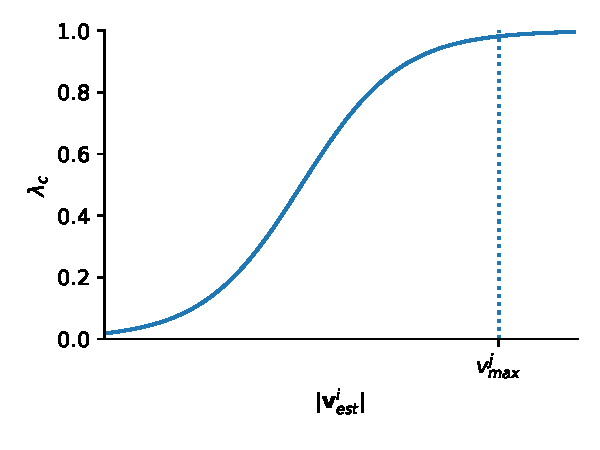
\includegraphics[width=0.6\textwidth]{figures/norm-trans.pdf}
\caption{\label{fig:norm-trans}The result of evaluating this function for an estimated object velocity is used as the normalizing factor for the translational residual from the constant motion assumption.}
\end{figure}

We make another adjustment to the objective function: as every landmark-feature pair creates a residual for a given frame, but there exist only a single constant motion residual, we scale the constant motion residual proportionally to the number of observations in a frame (or vice versa, the residuals of each observation needs to be inversely scaled by the number of total observations \(o_t\) in frame \(t\)).
Finally, we multiply both the translational and the rotational residual of the constant motion assumption by fixed object-specific (for object \(i\)) constants \(c^i_t\) and \(c^i_R\), respectively.
\cref{eq:bamot-final} gives the final objective function for the Bundle Adjustment optimization.

\begin{equation}
\label{eq:bamot-final}
    \min \sum_{n, t}\frac{1}{o_t}\rho(||\mathbf{p}_{t}^{n} - \pi({}^{o}_{c}\mathbf{T}^{t}{}^{o}\mathbf{P}_{n})||^2) 
+ \lambda_c \cdot c^i_t \cdot |\begin{bmatrix} \mathbf{I}^3 & \mathbf{0}^3 \\ \mathbf{0}^3 & \mathbf{0}^3 \end{bmatrix} \boldsymbol{\epsilon}_t|
+ c^i_R \cdot |\begin{bmatrix} \mathbf{0}^3 & \mathbf{0}^3 \\ \mathbf{0}^3 & \mathbf{I}^3 \end{bmatrix} \boldsymbol{\epsilon}_t|
\end{equation}

We employ the open-source framework g2o \cite{kummerleG2oGeneralFramework2011} for our object-level graph optimization.
BAMOT adapts a sliding window approach to limit the number of parameters in the optimization problem: 
the proposed system only performs \gls{ba} on the past \(n_w\) frames for a given object while it is active. 
The optimization keeps the oldest pose in this sliding window fixed s.t. the resulting trajectory remains connected.
Limiting the number of parameters, in turn, decreases runtime.

\subsection{Estimating OOBBs}
\label{sec:org9376cc2}
At every step, we estimate \glspl{oobb} in an online fashion, which we use for later performance evaluation.
As previously mentioned, an \gls{oobb} consists of a 3D location, the dimensions of an object, and the object's orientation w.r.t. its height (assumed to be parallel to gravity).
To estimate an object's location, we compute the entire object point cloud median and the current landmarks' median. We then take the mean of these two medians.
We use the object pose and landmark locations after \gls{ba} to benefit fully from this optimization result.
For objects that the system did not detect in a given frame, we only use the median of all existing landmarks as no notion of ``current'' landmarks exists.
To calculate the orientation, we use the direction of an estimated velocity vector. We base this velocity vector on the previous \(n_v\) frames: 
similar to our motion extrapolation method, we compute the relative translation in the current ego frame between the current frame and frame at time \(t_0 = t - \min(n_v, n_p)\) where \(n_p\) are the number of detections
of an object (i.e., the length of the track). We then project the resulting velocity vector onto the x,z-plane of the current camera coordinate system.
Finally, we calculate the angle between the projected velocity vector \(\tilde{\mathbf{v}}\) and the x-axis of the ego frame:
\begin{equation}
r_{y} = \text{arccos}(\begin{pmatrix}1 & 0 \end{pmatrix} \tilde{\mathbf{v}})
\end{equation}

This angle \(r_{y}\) is the \gls{oobb} orientation.

We do not estimate object dimensions. Instead, we employ constant dimensions per object class. 
We set these dimensions to roughly match the median dimensions of objects in the dataset we evaluate on.

\chapter{Results \label{results}}
\label{sec:orgab14fbb}
   The Appendix tabulates the system's hyperparameters' configuration (as discussed in \cref{method}) for the following results. 
The code is publicly available.\footnote{\url{https://github.com/AnselmC/bamot}}

\section{KITTI Dataset \label{kitti-dataset}}
\label{sec:org3c430b4}
   The KITTI benchmark suite \cite{geigerVisionMeetsRobotics2013}\footnote{\url{http://www.cvlibs.net/datasets/kitti/index.php}} encompasses datasets and evaluation procedures for various computer vision applications, 
including odometry, 3D object detection, and 2D multi-object tracking. The datasets are created by driving around a car through Karlsruhe (Germany), surrounding suburban areas, and highways. The result is a variety of real-world situations with alternating amounts of other traffic participants (e.g., cars, pedestrians, and cyclists). The vehicle is equipped with two grayscale cameras, two RGB cameras, a GPS sensor, an IMU sensor,
and a \gls{lidar} (see \cref{fig:kitti-car} for the setup). The authors calibrate the car's cameras and provide both raw and rectified (see \cref{epipolar-geometry}) image data and the corresponding calibration parameters.
Additionally, the datasets include the \gls{lidar} data and the ego vehicle's ground truth poses (derived from the GPS and IMU sensors). Different datasets provide further data specific to the task at hand.

\begin{figure}[htbp]
\centering
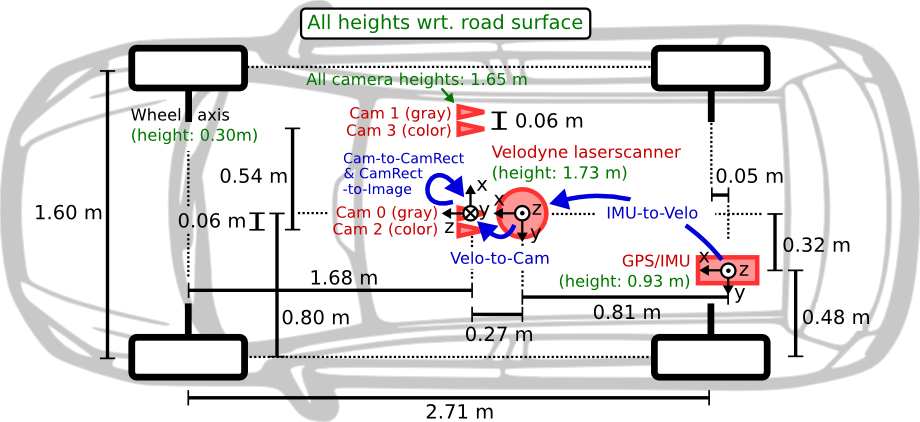
\includegraphics[width=0.75\textwidth]{figures/kitti-car.png}
\caption{\label{fig:kitti-car}The car setup for the KITTI dataset \cite{geigerVisionMeetsRobotics2013}.}
\end{figure}

We evaluate the proposed system on the multi-object tracking dataset.\footnote{\url{http://www.cvlibs.net/datasets/kitti/eval\_tracking.php}}
The dataset encompasses 21 training scenes, each of which includes ground truth object detections for every frame.
Each detection consists of a track ID (s.t. ground truth tracks are available), the \gls{oobb} for the detection, the class of the detected object, 
the 2D bounding box around the detection, and (in its multi-object tracking and segmentation extensions) 2D segmentation masks.
There are also 29 scenes for testing for which only the input data (i.e., images and LiDAR) are openly available.
Performance on this test set can only be evaluated by uploading results to the official KITTI benchmark servers.

\section{Quantitative results}
\label{sec:orge52f5ee}
    Although KITTI provides \gls{oobb} for detections and includes a benchmark for 3D \gls{mod} and 2D \gls{mot}, evaluation for 3D \gls{mot} is notably absent.
As mentioned in \cref{related-work}, \cite{wengBaseline3DMultiObject2019} introduced a benchmark for this purpose which is based on KITTI and uses adjusted CLEAR metrics (see \cref{clear-metrics})
with a 3D \gls{iou} similarity score.
Nonetheless, as such a non-generalized \gls{iou} doesn't take distance of non-overlapping bounding boxes into account (see \cref{matching-by-detection} for an explanation) 
we adopt a normalized 3D \gls{giou} \cite{rezatofighiGeneralizedIntersectionUnion2019} to calculate similarity: 

\begin{equation}
\label{eq:normed-giou}
S(d_{gt}, d_{est}) = \frac{1 + IoU(d_{gt}, d_{est}) - \frac{|C \setminus (d_{gt} \cup d_{est})|}{|C|}}{2}
\end{equation}

In \cref{eq:normed-giou}, \(d_{gt}\) is a ground truth detection in a given frame, \(d_{est}\) is an estimated detection, and \(C\) is the minimal \gls{oobb} which includes both \(d_{gt}\) and \(d_{est}\).

We evaluate system performance w.r.t. cars and pedestrians on both \gls{hota} \cite{luitenHOTAHigherOrder2021} and CLEAR \cite{bernardinEvaluatingMultipleObject2008}.
However, we set the system parameters to optimize for \gls{hota}. 
We then compare the results of \gls{bamot} to the LiDAR-based method AB3DMOT \cite{wengBaseline3DMultiObject2019} as the authors readily provide 3D tracking results.
We compare performance on the validation scenes of the learned system AB3DMOT from KITTI: \(\{1, 6, 8, 10, 12, 13, 14, 15, 16, 18, 19\}\).
Because AB3DMOT depends on confidence threshold filtering, we evaluate using the confidence threshold that maximizes its performance for the given metric.

We evaluate via the official scripts of \gls{hota}\footnote{\url{https://github.com/JonathonLuiten/TrackEval}} with a custom implementation for 3D \gls{oobb} with the above mentioned normalized 3D \gls{giou}.\footnote{based on work from Nikita Korobov (\url{https://github.com/nekorobov/HOTA-metrics})} 
The official 2D KITTI evaluation removes ``acceptable'' \gls{fp} detections in crowded areas or smaller than 25 pixels. The script determines these \gls{fp} detections by matching estimated and ground-truth detections
and considering all matches with \gls{iou} scores below 0.5 as unmatched and potential \gls{fp}.
This removal arguably makes sense in 2D (but it also originates from the fact that the original CLEAR metric evaluation only counts a detection with an \gls{iou} greater than 0.5 as a \gls{tp}). 
However, for small (i.e., far away) detections, the depth estimates are less accurate than their 2D projections. 
Thus, considering detections with normalized 3D \gls{giou} similarities below 0.5 as unmatched and then deeming them as \glspl{fp} if they fall slightly below the 25-pixel height harms performance.
Since this preprocessing step is supposed to be a positive contribution to overall performance in its original application, and this is not the case by one-to-one application in 3D, we adjust the threshold to be 0.25 vs. 0.5. 
\cref{tab:thresholds} shows that this has a positive, if negligible, effect on the method we compare against w.r.t. to the primary evaluation metric \gls{hota}.

The confidence thresholds determined to maximize AB3DMOT performance on 3D \gls{giou} are 2.34 for cars (both \gls{hota} and \gls{mota}) and 1.50 (\gls{hota})/2.0 (\gls{mota}) for pedestrians (note that AB3DMOT does not normalize confidences).

\begin{table}
\centering
\adjustbox{max width=\linewidth} {

\begin{tabular}{llrllllll}
 & HOTA & DetA & AssA & DetRe & DetPr & AssRe & AssPr & LocA\\
\hline
\cite{wengBaseline3DMultiObject2019} (car, \(\alpha \geq 0.5\)) & 74.4 & 72.5 & \textbf{76.9} & 79.1 & 83.8 & \textbf{79.9} & \textbf{91.0} & \textbf{89.0}\\
\cite{wengBaseline3DMultiObject2019} (car, \(\alpha \geq 0.25\)) & \textbf{74.5} & \textbf{72.6} & 76.8 & 79.1 & \textbf{83.9} & \textbf{79.9} & 90.9 & \textbf{89.0}\\
\cite{wengBaseline3DMultiObject2019} (car, \(\alpha \geq 0.1\)) & 74.3 & 72.5 & 76.6 & \textbf{79.2} & 83.7 & \textbf{79.9} & 90.7 & 88.9\\
\hline
\cite{wengBaseline3DMultiObject2019} (ped., \(\alpha \geq 0.5\)) & \textbf{55.5} & 55.3 & \textbf{55.9} & \textbf{59.9} & \textbf{76.0} & \textbf{57.5} & \textbf{84.4} & \textbf{82.5}\\
\cite{wengBaseline3DMultiObject2019} (ped., \(\alpha \geq 0.25\)) & \textbf{55.5} & 55.3 & \textbf{55.9} & \textbf{59.9} & \textbf{76.0} & \textbf{57.5} & \textbf{84.4} & \textbf{82.5}\\
\cite{wengBaseline3DMultiObject2019} (ped., \(\alpha \geq 0.1\)) & \textbf{55.5} & \textbf{55.4} & \textbf{55.9} & \textbf{59.9} & \textbf{76.0} & \textbf{57.5} & 84.3 & 82.4\\
\end{tabular}

}
\caption{Adjusting the preprocessing similarity threshold $\alpha$ for filtering \gls{fp} to match the new setting (i.e., normalized 3D \gls{giou} vs. 2D \gls{iou}) also has a slightly positive effect on AB3DMOT}.
\label{tab:thresholds}
\end{table}

\subsection{HOTA}
\label{sec:org6245977}
    \cref{tab:hota} tabulates a performance comparison between AB3DMOT and \gls{bamot}. As to be expected, the LiDAR-based method outperforms our vision-based method.
This superiority arises from the fact that the underlying depth data from \gls{lidar} is far more accurate than triangulated landmarks from RGB data. 
Additionally, the discrepancy in accuracy increases with distance.
Finally, the \gls{lidar} input density compared to feature-based landmark sparsity allows for more accurate location and shape estimates and thus inferred bounding boxes. 
This not only affects the location accuracy LocA (\cref{eq:hota-loca}) but also the detection accuracy DetA (\cref{eq:hota-deta}), association accuracy AssA (\cref{eq:hota-assa}),
and thus \gls{hota} (\cref{eq:hota}).
This widespread effect comes from the similarity score (in our case given in \cref{eq:normed-giou}) upon which all metrics are based.
The maximally achievable similarity \(S_{max}\) of a given \gls{mot} system gives an upper bound for \gls{hota} and its derivative metrics.
This is easily shown. For a given threshold \(\alpha\), 

\begin{equation}
\text{LocA}_\alpha = \frac{\sum_{c \in \{TP_\alpha\}}S(c)}{|\{TP_\alpha\}|} \leq S_{max}.
\end{equation}
Additionally, for \(\alpha > S_{max}\),

\begin{equation}
\text{LocA}_{\alpha > S_{max}} = 0.
\end{equation}

This inequality follows from assuming (at best) constant similarities \(S_{max}\) for all \gls{tp} detections.
Integrating over \(\alpha\) to calculate \(\text{LocA}\), then yields 
\begin{equation}
\text{LocA} = \int_0^1\text{LocA}_\alpha d\alpha \leq S_{max}^2.
\end{equation}

Similarly, for \(\text{DetA}\) the upper-bound for a single threshold \(\alpha\) is 1: 
\begin{equation}
    \text{DetA}_\alpha = \frac{|\{TP_\alpha\}|}{|\{TP_\alpha\}|+|\{FN_\alpha\}|+|\{FP_\alpha\}|} \leq 1.
\end{equation}
Again, assuming a maximally attainable similarity score \(S_{max}\), it follows that 
\begin{equation}
\text{DetA}_{\alpha > S_{max}} = 0
\end{equation}
and thus 
\begin{equation}
 \text{DetA} = \int_0^1\text{DetA}_\alpha d\alpha \leq S_{max}.
\end{equation}

The same inequality holds for \(\text{AssA}\) and \gls{hota}, i.e., \(\text{AssA} \leq S_{max}\) and \(\text{HOTA} \leq S_{max}\).

In practice, \(\text{LocA}\) is larger than the other measures as it disregards \glspl{fn} and \glspl{fp}. 
Nonetheless, the presented inequalities give a sense of how high similarity scores strongly influence all evaluation metrics' dimensions.

When comparing our system for the car object class to AB3DMOT, one also sees that while the detection accuracy decreases by \(\frac{65.8-35.8}{65.8} \approx 46 \%\), association accuracy merely decreases by
\(\frac{77.8-48.2}{77.8} \approx 38 \%\). This indicates that \gls{bamot} comparatively improves association.
Another key insight is that tracking performance w.r.t. pedestrians is considerably worse. 
This inferiority has two reasons. First, our sparse feature-based approach detects fewer features on smaller objects which negatively affects both localization accuracy and robust association.
Second, people violate our model's non-rigidity assumption, i.e., landmarks detected on arms and legs change their location w.r.t. the fixed object coordinate-frame.
Non-static landmarks lead to either estimating wrong object poses via \gls{pnp} or removing such landmarks, thus increasing pedestrian point clouds' sparsity.
Hence, unless pedestrians are fully visible (i.e., landmarks on the more-or-less rigid torso can be redetected and used for localization and association) or stationary, our system has trouble tracking them over time.
It often loses track of the pedestrian and reinitializes a new object track. 
This instability results in a lower association accuracy vs. detection accuracy for pedestrians.
For cars the opposite is true: association accuracy is higher than detection accuracy.
Additionally, the localization accuracy (i.e., average similarity score for \gls{tp} detections at a given similarity threshold) for pedestrians is only slightly below that of cars (65.0 vs. 66.6).

\begin{table}
\centering
\adjustbox{max width=\linewidth} {

\begin{tabular}{lllllllll}
 & HOTA & DetA & AssA & DetRe & DetPr & AssRe & AssPr & LocA\\
\hline
\textbf{BAMOT} (car) & 40.7 & 35.8 & 48.2 & 40.9 & 49.0 & 53.8 & 59.9 & 66.6\\
\cite{wengBaseline3DMultiObject2019} (car) & \textbf{71.3} & \textbf{65.8} & \textbf{77.8} & \textbf{83.1} & \textbf{71.5} & \textbf{81.5} & \textbf{90.0} & \textbf{88.5}\\
\hline
\textbf{BAMOT} (ped.) & 19.7 & 22.7 & 18.4 & 27.2 & 39.6 & 21.2 & 46.0 & 65.0\\
\cite{wengBaseline3DMultiObject2019} (ped.) & \textbf{55.5} & \textbf{55.3} & \textbf{55.9} & \textbf{59.9} & \textbf{76.0} & \textbf{57.5} & \textbf{84.4} & \textbf{82.5}\\
\end{tabular}

}
\caption{As expected, the LiDAR-based AB3DMOT is superior to our vision-based approach. However, the superiority especially stems from more accurate localization.
Because we implement a feature-based approach for both 3D localization and association, the resulting sparsity makes it harder to track smaller, non-rigid pedestrians than cars.}
\label{tab:hota}
\end{table}


\cref{tab:hota-ablation} tabulates how various parts of \gls{bamot} influence overall performance. 
We alternately ``switch-off'' the following characteristics:

\begin{itemize}
\item improving TrackR-CNN's association with our three-step association pipeline detailed in \cref{detection-track-assoc}
\item initializing tracks only when the number of successfully triangulated landmarks surpasses a threshold
\item the local constant motion error term in object-level \gls{ba} (see \cref{object-lvl-ba})
\item keeping tracks in memory and thus, ``re-matchable'', after not being successfully localized for a specified number of frames
\end{itemize}

For cars, our association pipeline's effect is a \textasciitilde{}16\% improvement in association accuracy, translating to a \textasciitilde{}9\% increase in the resulting \gls{hota} score. 
This improvement comes at a slight (arguably negligible) cost in localization accuracy and, thus, in detection accuracy. 

However, our association pipeline hurts pedestrian tracking. 
While association accuracy increases slightly (the number of \glspl{fpa} significantly decreases, leading to much higher association recall), detection accuracy decreases.
This is because we are often unable to successfully associate a detection to a track in 3D and, thus, forgo adding the detection.
Using the image-based associations from TrackR-CNN will not result in this behavior leading to a performance increase of \textasciitilde{}5\% for \gls{hota}.
This is not surprising and another effect of our sparse object representation approach.

The constant motion error term in object-level \gls{ba} penalizes non-smooth trajectories. 
This has a significant effect on pedestrians since they contain a larger outlier ratio w.r.t. feature-landmark associations because of their non-rigidity.
This mainly manifests itself in the resulting detection accuracy, which increases by \textasciitilde{}97\%.
Thus, they benefit from this regularizing error term. For cars, the effect is negligible.

The removal of robust initialization (i.e., initializing new objects once the system triangulates a single landmark) results in overall more but inaccurate detections.
Comparatively, for low similarity thresholds, this increases \glspl{tp} and decreases \glspl{fn} leading to higher detection recall. 
However, for higher similarity thresholds, such inaccurate detections lead to \glspl{fp} and \glspl{fn}, resulting in lower detection precision and lower recall (compared to robust initialization).
Thus, although both metrics are affected, the effect on detection precision is more severe in total as it is not counter-balanced by the improved recall at lower \(\alpha\).
We plot the impact of the different number of minimum landmarks for initializing cars in \cref{fig:min-lm-plot}.

Lastly, retaining tracks after they are lost has a more significant effect on association vs. detection. 
This comparative improvement in associating detections is because \gls{bamot} can reassociate such lost tracks to detections in the future, 
increasing the \glspl{tpa} for a given detection (i.e., avoiding an identity switch).
\cref{fig:keep-track-plot} shows the effect of retaining a car track for a differing number of frames before removing it from the system.
While the outcome is positive for both cars and pedestrians overall, one can see that the detection and association precision, as well as the localization accuracy improves when we delete tracks quickly.
This is because we have less false positive detections that result from not being able to track an existing track and, thus, estimating its position in a given frame incorrectly.
However, if we continuously reinitialize tracks, we can more accurately localize each detection as the localization is unconstrained from past detections (and associated landmarks and object poses).

\begin{table}
\centering
\adjustbox{max width=\linewidth}{

\begin{tabular}{lllllllll}
 & HOTA & DetA & AssA & DetRe & DetPr & AssRe & AssPr & LocA\\
\hline
\textbf{BAMOT} (car) & \textbf{40.7} & 35.8 & \textbf{48.2} & 40.9 & 49.0 & \textbf{53.8} & 59.9 & 66.6\\
no impr. assoc. (car) & 37.2 \(\downarrow\) & \textbf{35.9} \(\uparrow\) & 41.2 \(\downarrow\) & 41.6 \(\uparrow\) & 47.7 \(\downarrow\) & 52.6 \(\downarrow\) & 52.5 \(\downarrow\) & 66.4 \(\downarrow\)\\
no const. motion (car) & 40.4 \(\downarrow\) & 36.1 \(\uparrow\) & 47.1 \(\downarrow\) & 40.7 \(\downarrow\) & 50.3 \(\uparrow\) & 52.7 \(\downarrow\) & 60.4 \(\uparrow\) & 66.9 \(\uparrow\)\\
no track retention (car) & 39.1 \(\downarrow\) & 35.8 - & 44.8 \(\downarrow\) & 39.8 \(\downarrow\) & \textbf{51.2}  \(\uparrow\) & 49.2 \(\downarrow\) & \textbf{61.8}  \(\uparrow\) & \textbf{66.9} \(\uparrow\)\\
no robust init. (car) & 39.1 \(\downarrow\) & 35.9 \(\uparrow\) & 44.6 \(\downarrow\) & \textbf{42.7} \(\uparrow\) & 46.0 \(\downarrow\) & 50.2 \(\downarrow\) & 57.9  \(\downarrow\) & 66.0  \(\downarrow\)\\
none of the above (car) & 35.0 \(\downarrow\) & 34.9 \(\downarrow\) & 37.3 \(\downarrow\) & 40.2 \(\downarrow\) & 46.3 \(\downarrow\) & 49.0 \(\downarrow\) & 48.5  \(\downarrow\) & 65.6  \(\downarrow\)\\
\hline
\textbf{BAMOT} (ped.) & 19.7 & 22.7 & 18.4 & 27.2 & 39.6 & 21.2 & 46.0 & 65.0\\
no impr. assoc. (ped.) & \textbf{20.7} \(\uparrow\) & \textbf{24.3} \(\uparrow\) & 18.1 \(\downarrow\) & \textbf{30.7} \(\uparrow\) & 36.4 \(\downarrow\) & \textbf{29.4}  \(\uparrow\) & 27.6 \(\downarrow\) & 64.2     \(\downarrow\)\\
no const. motion (ped.) & 13.7   \(\downarrow\) & 11.5  \(\downarrow\) & 17.0  \(\downarrow\) & 12.9  \(\downarrow\) & 35.6  \(\downarrow\) & 19.3   \(\downarrow\) & 44.4 \(\downarrow\) & 63.6    \(\downarrow\)\\
no track retention (ped.) & 11.6   \(\downarrow\) & 11.4  \(\downarrow\) & 12.5  \(\downarrow\) & 12.0  \(\downarrow\) & \textbf{45.0} \(\uparrow\) & 13.3   \(\downarrow\) & \textbf{59.0}     \(\uparrow\) & \textbf{65.4}  \(\uparrow\)\\
no robust init. (ped.) & 14.6   \(\downarrow\) & 12.0  \(\downarrow\) & 18.6  \(\uparrow\) & 13.4  \(\downarrow\) & 36.0   \(\downarrow\) & 20.9   \(\downarrow\) & 45.9   \(\downarrow\) & 63.5   \(\downarrow\)\\
none of the above (ped.) & 15.5   \(\downarrow\) & 12.4  \(\downarrow\) & \textbf{19.8} \(\uparrow\) & 13.7  \(\downarrow\) & 37.0  \(\downarrow\) & 28.8  \(\uparrow\) & 30.7     \(\downarrow\) & 64.0      \(\downarrow\)\\
\end{tabular}

}
\caption{An ablation study comparing how different high-level notions of our system influence its overall performance.
Overall \gls{bamot} benefits from a $\sim17\%$ (cars) and $\sim27\%$ (pedestrians) performance increase from using improved associations, robustly initializing new tracks, assuming constant local motion in object-level \gls{ba},
and keeping lost tracks in memory s.t. \gls{bamot} can redetect them.}
\label{tab:hota-ablation}
\end{table}

\begin{figure}[htbp]
\centering
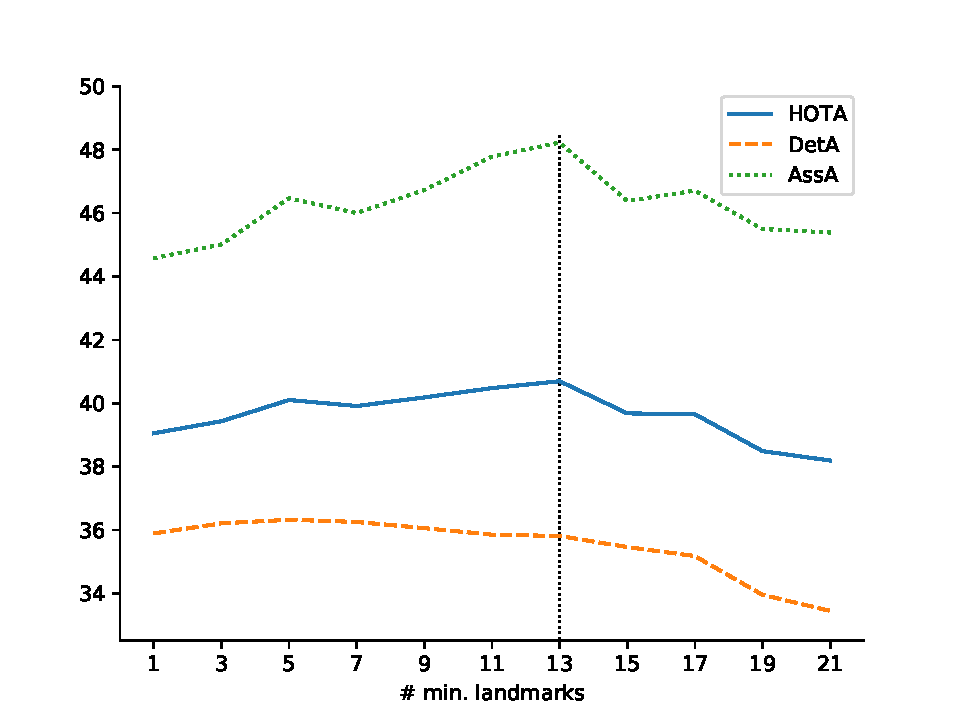
\includegraphics[width=0.9\textwidth]{figures/min-lm-plot.pdf}
\caption{\label{fig:min-lm-plot}Robustly initializing objects with a minimal number of required landmarks leads to improved association and, thus, improved \gls{hota}. However, as the number increases, the \gls{tp} detection count decreases along with performance. This plot shows how the number of minimum landmarks affects our system's car tracking performance. \emph{Best viewed in color}.}
\end{figure}


\begin{figure}[htbp]
\centering
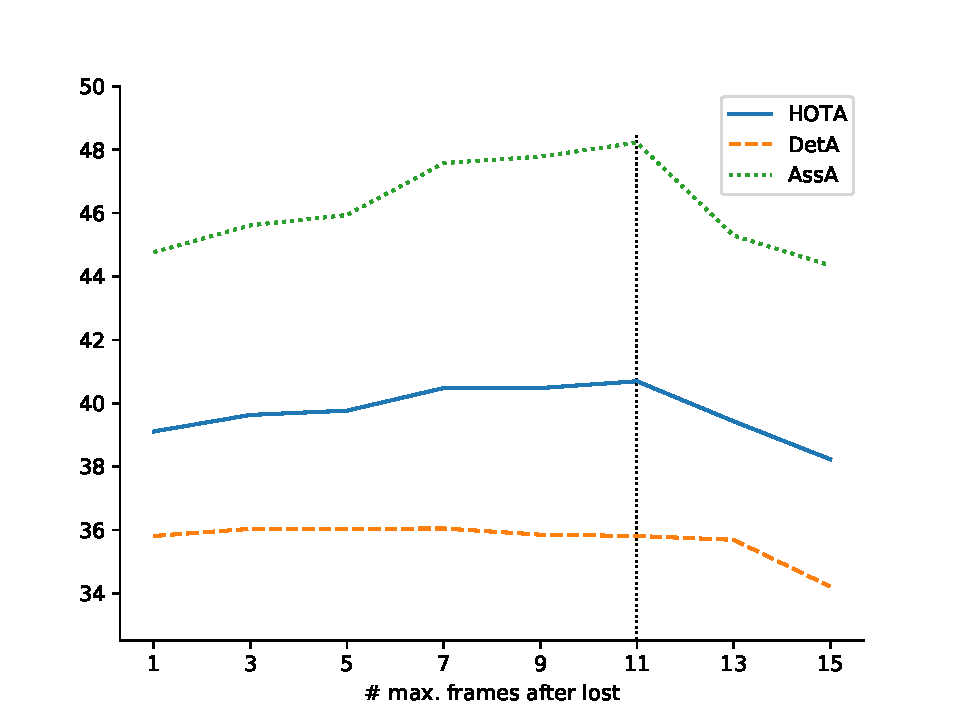
\includegraphics[width=0.9\textwidth]{figures/keep-track-plot.pdf}
\caption{\label{fig:keep-track-plot}Keeping tracks after the system cannot associate a 2D detection to it (e.g., because the object is occluded), allows us to associate future detections to a track. Again, there is a trade-off: if we keep tracks too long in memory, we increase the likelihood of erroneously matching detections of new tracks to old tracks. This plot shows how this trade-off manifests itself in the performance for 3D multi-object tracking for cars. \emph{Best viewed in color}.}
\end{figure}


\subsection{MOTA}
\label{sec:org4d21e64}
    For completeness, we also evaluate 3D \gls{mota}. 
\cref{tab:clear-car} and \cref{tab:clear-ped} show results based on the CLEAR \cite{bernardinEvaluatingMultipleObject2008} metrics (see \cref{clear-metrics}). 
The 2D CLEAR metrics deem a detection a \gls{tp} if its \gls{iou} is at least 0.5. Unlike \gls{hota}, the CLEAR metrics only evaluate a single similarity threshold.
If we keep this threshold for 3D \gls{giou}, our vision-based method performs very poorly as many estimated detections ``fall under the table'' and get counted as both a \gls{fp} and a \gls{fn}.
However, if we count detections with a similarity score of at least 0.25 (\(S \geq \alpha = 0.25\)), this paints a very different picture. 
For cars and pedestrians, the MOTA score increases by large margins: from \(-0.0954\) to \(69.4\) for cars and from \(-18.5\) to \(31.6\) for pedestrians.
This is because, at a lower minimally required similarity, many more estimated detections can be matched to their ground truth counterparts, thus increasing \glspl{tp}.
At the same time, both MOTP scores drop. The reasoning being that MOTP measures the average similarity of \glspl{tp} detections. At a high minimum similarity threshold, this is necessarily higher, as only 
very precise detections are considered. 
Pedestrians exhibit fewer such precise \glspl{oobb} compared to cars. This leads to both lower MOTA and MOTP performance.
Disabling the minimum similarity score altogether still increases MOTA; however, it also decreases MOTP to the same degree, arguably rendering that final step inconsequential.
The effect for AB3DMOT is less severe as its \gls{oobb} estimates are decidedly more accurate due to the precision of \gls{lidar}.

\begin{table}
\centering
\adjustbox{max width=\linewidth} {

\begin{tabular}{lrrrrrrr}
 & MOTA & MOTP & MT (\%) & PT (\%) & ML (\%) & IDSW & FRAG\\
\hline
BAMOT  (\(\alpha=0.5\)) & -0.0954 & 62.2 & 4.9 & 54.6 & 40.5 & 21 & 421\\
\cite{wengBaseline3DMultiObject2019} (\(\alpha=0.5\)) & 81.0 & 88.1 & 71.9 & 27.0 & 1.08 & 22 & 149\\
\hline
BAMOT  (\(\alpha=0.25\)) & 69.4 & 52.1 & 53.5 & 38.4 & 8.11 & 39 & 92\\
\cite{wengBaseline3DMultiObject2019} (\(\alpha=0.25\)) & 81.1 & 87.6 & 71.9 & 27.1 & 1.08 & 29 & 147\\
\hline
BAMOT  (\(\alpha=0\)) & 76.6 & 48.9 & 61.1 & 34.1 & 4.86 & 67 & 72\\
\cite{wengBaseline3DMultiObject2019} (\(\alpha=0\)) & 83.0 & 81.9 & 77.8 & 22.2 & 0 & 129 & 159\\
\end{tabular}

}
\caption{ Comparison of cars' performance on the KITTI dataset via the detection-biased CLEAR metrics using 3D GIoU as a similarity measure.
When setting the minimum threshold $\alpha$ to 0.5, the evaluation disregards many detections. The CLEAR metrics then count each unmatched detection \emph{both} as a TP and as a FN, resulting in a low MOTA score.}
\label{tab:clear-car}
\end{table}

\begin{table}
\centering
\adjustbox{max width=\linewidth} {

\begin{tabular}{lrrrrrrr}
 & MOTA & MOTP & MT (\%) & PT (\%) & ML (\%) & IDSW & FRAG\\
\hline
BAMOT  (\(\alpha=0.5\)) & -18.5 & 61.0 & 4.23 & 45.8 & 50 & 259 & 497\\
\cite{wengBaseline3DMultiObject2019} (\(\alpha=0.5\)) & 66.7 & 80.5 & 44.4 & 40.8 & 14.8 & 85 & 235\\
\hline
BAMOT  (\(\alpha=0.25\)) & 31.6 & 48.2 & 21.1 & 60.6 & 18.3 & 366 & 355\\
\cite{wengBaseline3DMultiObject2019} (\(\alpha=0.25\)) & 66.9 & 79.9 & 45.1 & 40.8 & 14.1 & 88 & 233\\
\hline
BAMOT  (\(\alpha=0\)) & 58.7 & 33.1 & 33.1 & 53.5 & 13.4 & 326 & 242\\
\cite{wengBaseline3DMultiObject2019} (\(\alpha=0\)) & 68.8 & 69.6 & 48.6 & 39.4 & 12.0 & 156 & 251\\
\end{tabular}

}
\caption{For pedestrians, the effect of setting the minimum threshold $\alpha$ below 0.5 has a similar effect as it does for cars.
Overall, pedestrian tracks are often incorrectly tracked, as can be seen in the large number of IDSWs.}
\label{tab:clear-ped}
\end{table}




\section{Qualitative results}
\label{sec:org1975eeb}
   This section discusses and illustrates the qualitative results of this work. 
We create visualizations with Open3D \cite{zhouOpen3DModernLibrary2018} \footnote{\url{http://open3d.org}}.

As stated above, \gls{bamot} can track cars significantly better than small, non-rigid people. 
However, as our system orients bounding boxes based on the object's velocity vector, the orientation and detection accuracy increase as an object continues to be tracked for multiple frames and has an estimated velocity.
Additionally, the localization depends on the accuracy of triangulated landmarks and the object's distance from the camera.
\cref{fig:bounding-box-regression} shows how the orientation estimate improves for both close and far away objects as the system tracks them for a longer time; 
the figure also demonstrates how the camera's distance influences localization accuracy.

The dependency of orientation estimates on accurate velocity vectors results in a problem for stationary objects: here, the estimated movement of the object in 3D space is small but present, s.t. orientation estimates
are erroneous, resulting in imprecise \glspl{oobb}. Aligning \glspl{oobb} based on the geometry of the point cloud could result in improved alignment in such cases.
\cref{fig:stationary-objects} gives examples of the difficulties \gls{bamot} has with parked cars. Incorrect velocity vectors are less of an issue for pedestrians since \gls{oobb} orientation consists only of the yaw (i.e., rotation w.r.t. gravity) and
pedestrians have similar dimensions in the relevant axes.

\begin{figure}[htbp]
\centering
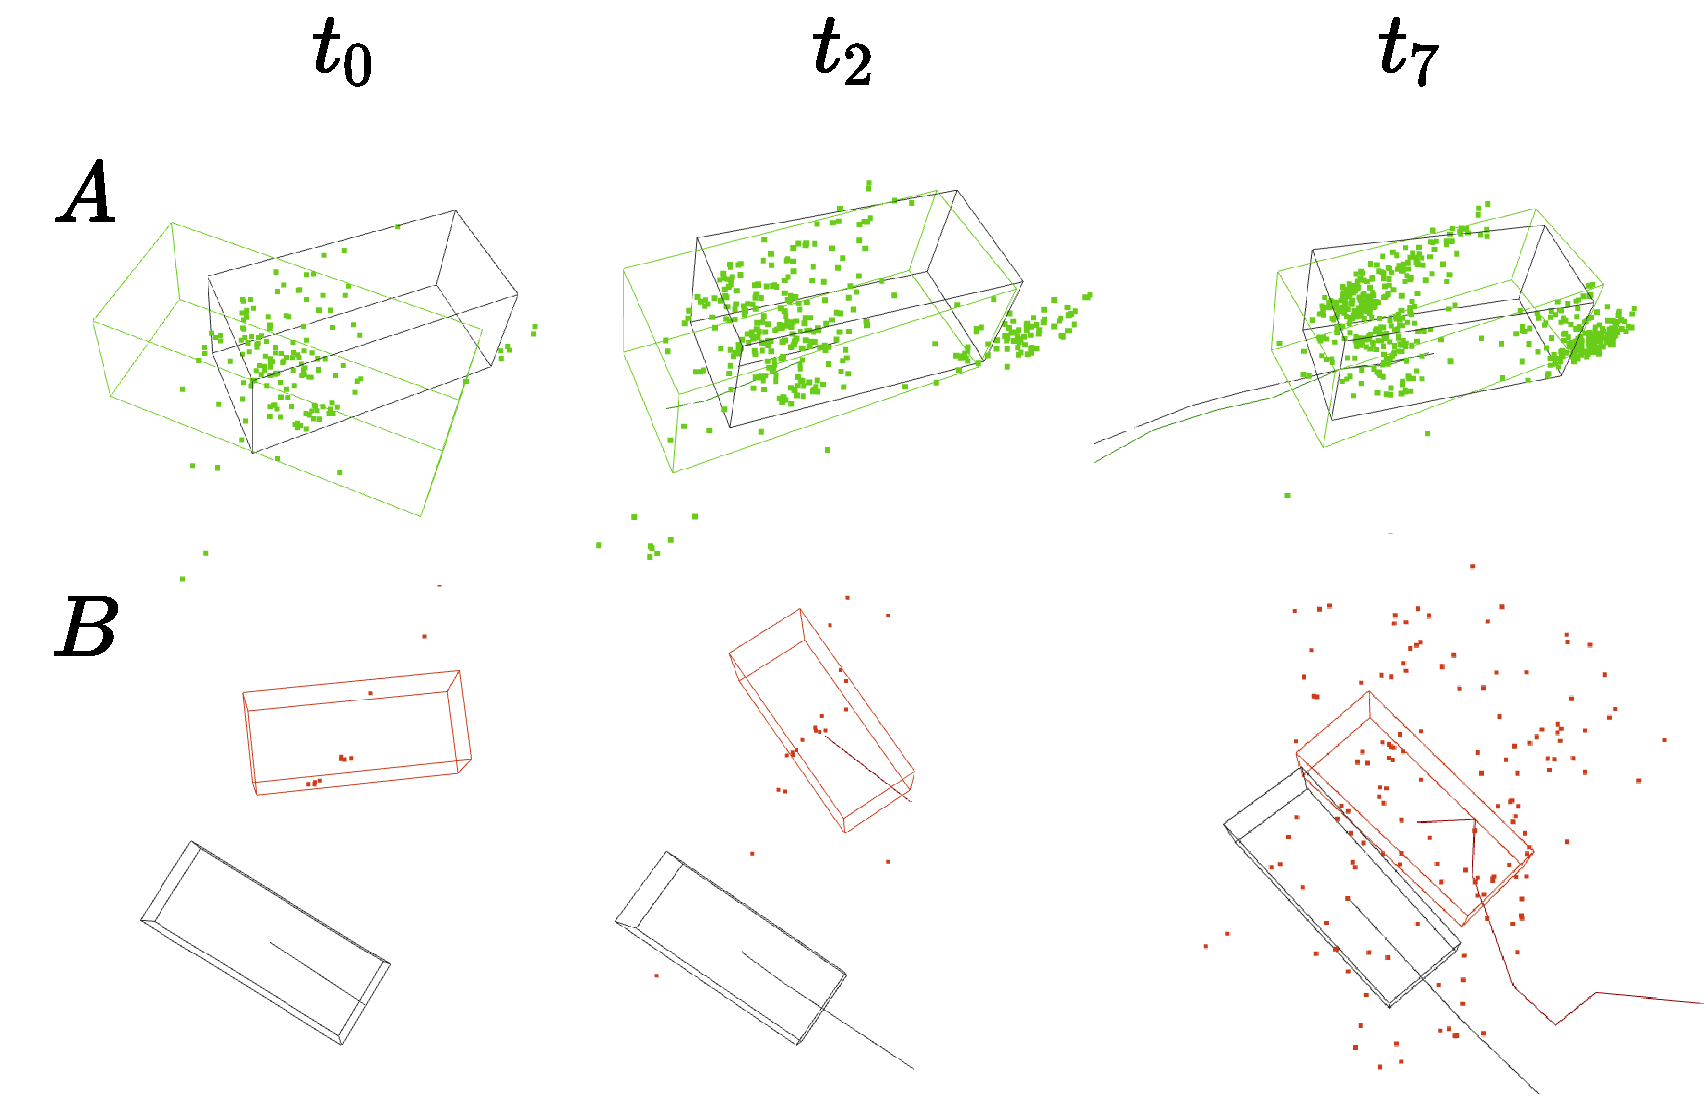
\includegraphics[width=\textwidth]{figures/bounding-box-regression.pdf}
\caption{\label{fig:bounding-box-regression}This figure demonstrates how the length of an object track and its distance to the camera influences the accuracy of \glspl{oobb}. \(t_0\) is the first frame containing the object detection. \(t_2\) and \(t_7\) show the object two and seven frames after initialization, respectively. Ground truth \glspl{oobb} and ground truth trajectories are drawn in black, estimated \gls{oobb} and trajectories in color. \emph{Top (A):} For close objects (approx. up to 20 times the stereo camera baseline), the localization of triangulated landmarks is precise. Additionally, as the system observes the object for several frames, the orientation of the bounding box improves. \emph{Bottom (B):} For far-away objects (\textasciitilde{}30m in this example), \gls{bamot} triangulates fewer and less-precise landmarks resulting in an inaccurate \gls{oobb}. Still, the estimate improves as more observations of the object are added. \emph{Best viewed in color}.}
\end{figure}

\begin{figure}[htbp]
\centering
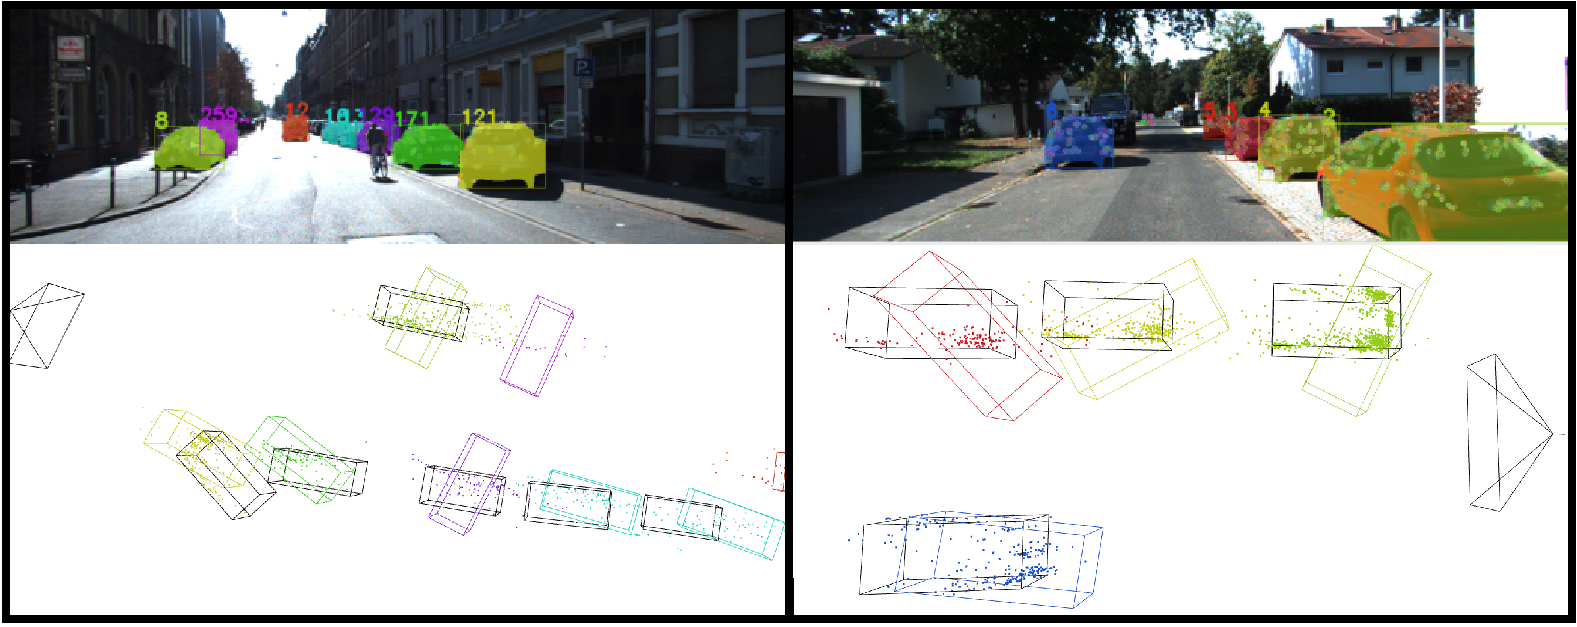
\includegraphics[width=\textwidth]{figures/stationary-objects.pdf}
\caption{\label{fig:stationary-objects}Estimating orientation from a velocity vector does not work for stationary objects. Ground truth \glspl{oobb} and trajectories are in black; their estimated counterparts are in color. \emph{Best viewed in color}.}
\end{figure}

\cref{fig:qualitative-scene} illustrates how the system can handle varying degrees of difficulties in \gls{mot}. Objects in the image domain (and potentially also detected by the object detector)
are not initialized by the system if not enough landmarks can be successfully triangulated. 
Even for initialized objects, one can see the landmark count's significant influence on its localization accuracy. 
Furthermore, for objects with several frames-long trajectories, the orientation of the sliding-window velocity vector accurately estimates the ground truth orientation.
Additionally, even if objects leave the image domain, \gls{bamot} continues to know their estimated locations in 3D space. 
This memorization has the negative side effect of \gls{fp} detections. Although we do not record not-in-view detections, objects leave our field-of-view typically after KITTI considers them gone.

\begin{figure}[htbp]
\centering
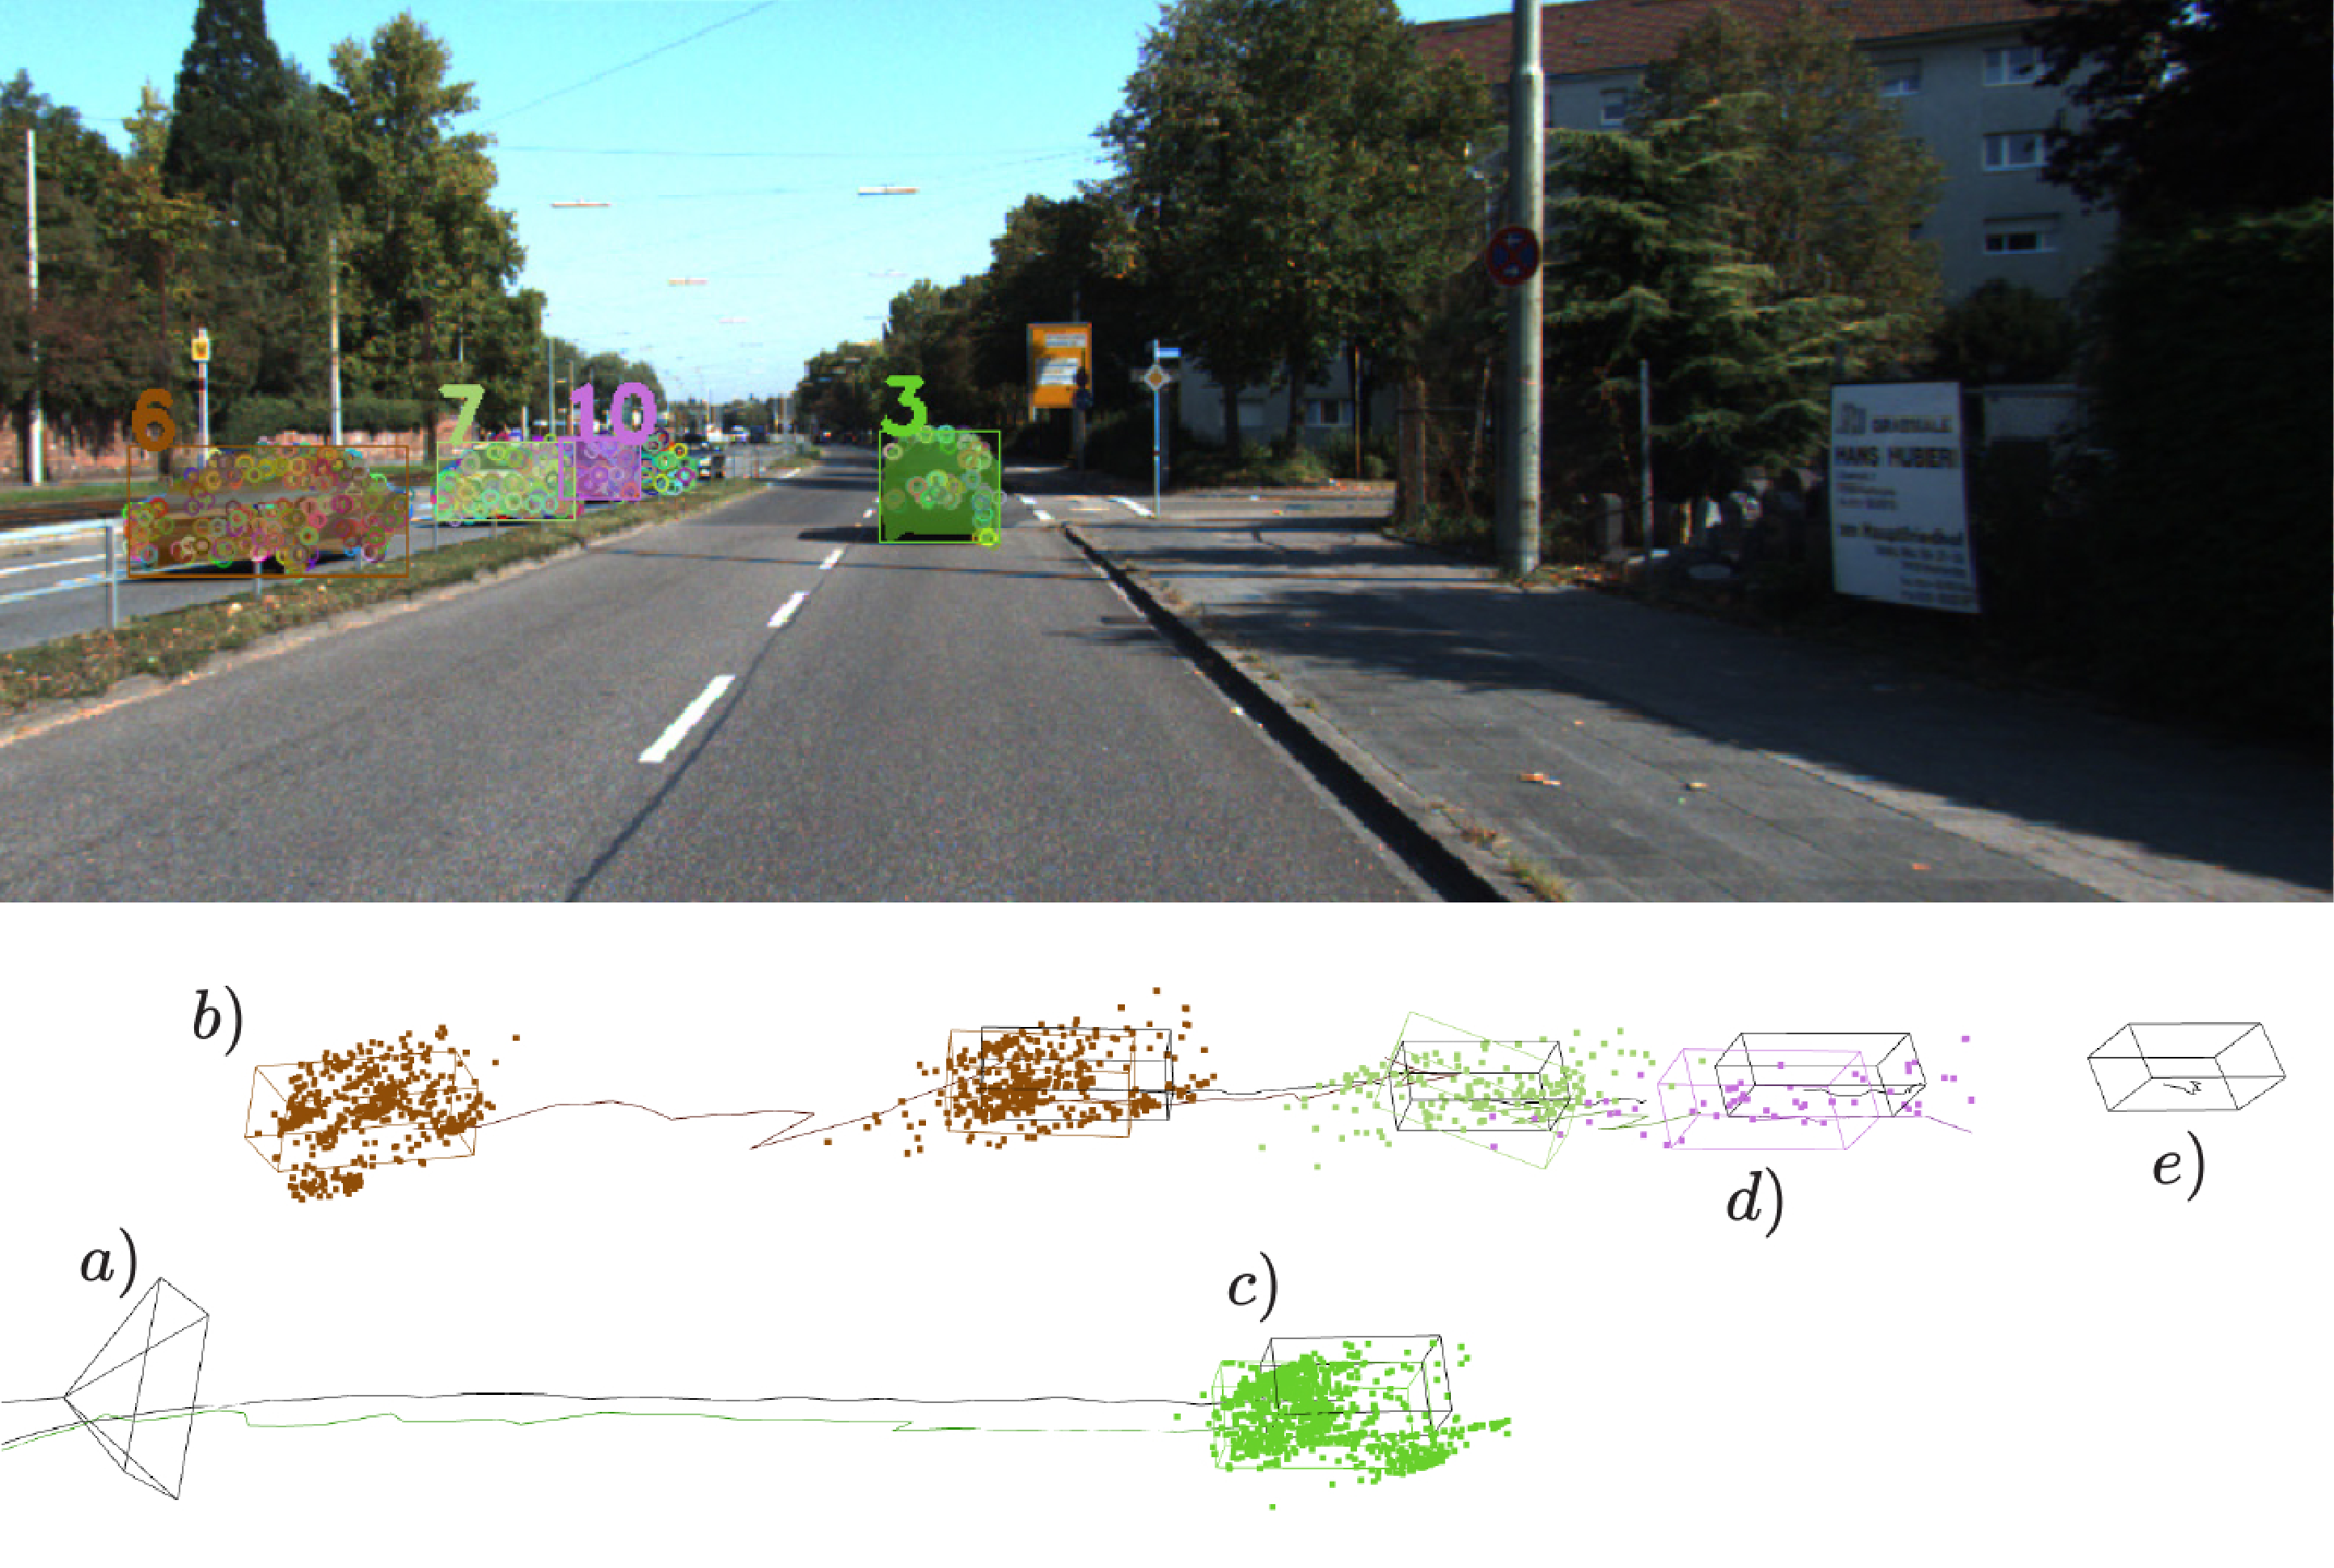
\includegraphics[width=\textwidth]{figures/qualitative-scene-stacked.pdf}
\caption{\label{fig:qualitative-scene}\emph{Top}: The current frame including the detected object segmentation masks and the associated object track IDs. Additionally, we draw the extracted ORB features onto the image. \emph{Bottom}: A 3D visualization of the ego-vehicle (a)), the ground truth \glspl{oobb} and trajectories (black), and the estimated object tracks (colorized). b) Even if the object leaves the image domain (no ground truth box exists) \gls{bamot} continues to track it for several frames and can reassociate it. c) A non-occluded object that isn't too far away and has been tracked for several frames is accurately (for vision-based systems) estimated, whereas objects with fewer landmarks exhibit less precise localization (d)). e) If we cannot triangulate enough landmarks, the system does not initialize an object even if detected in the image domain. \emph{Best viewed in color.}}
\end{figure}

\cref{fig:more-scenes} visualizes several other examples of our system's tracking capabilities w.r.t. different traffic scenarios for cars.
\begin{figure}[htbp]
\centering
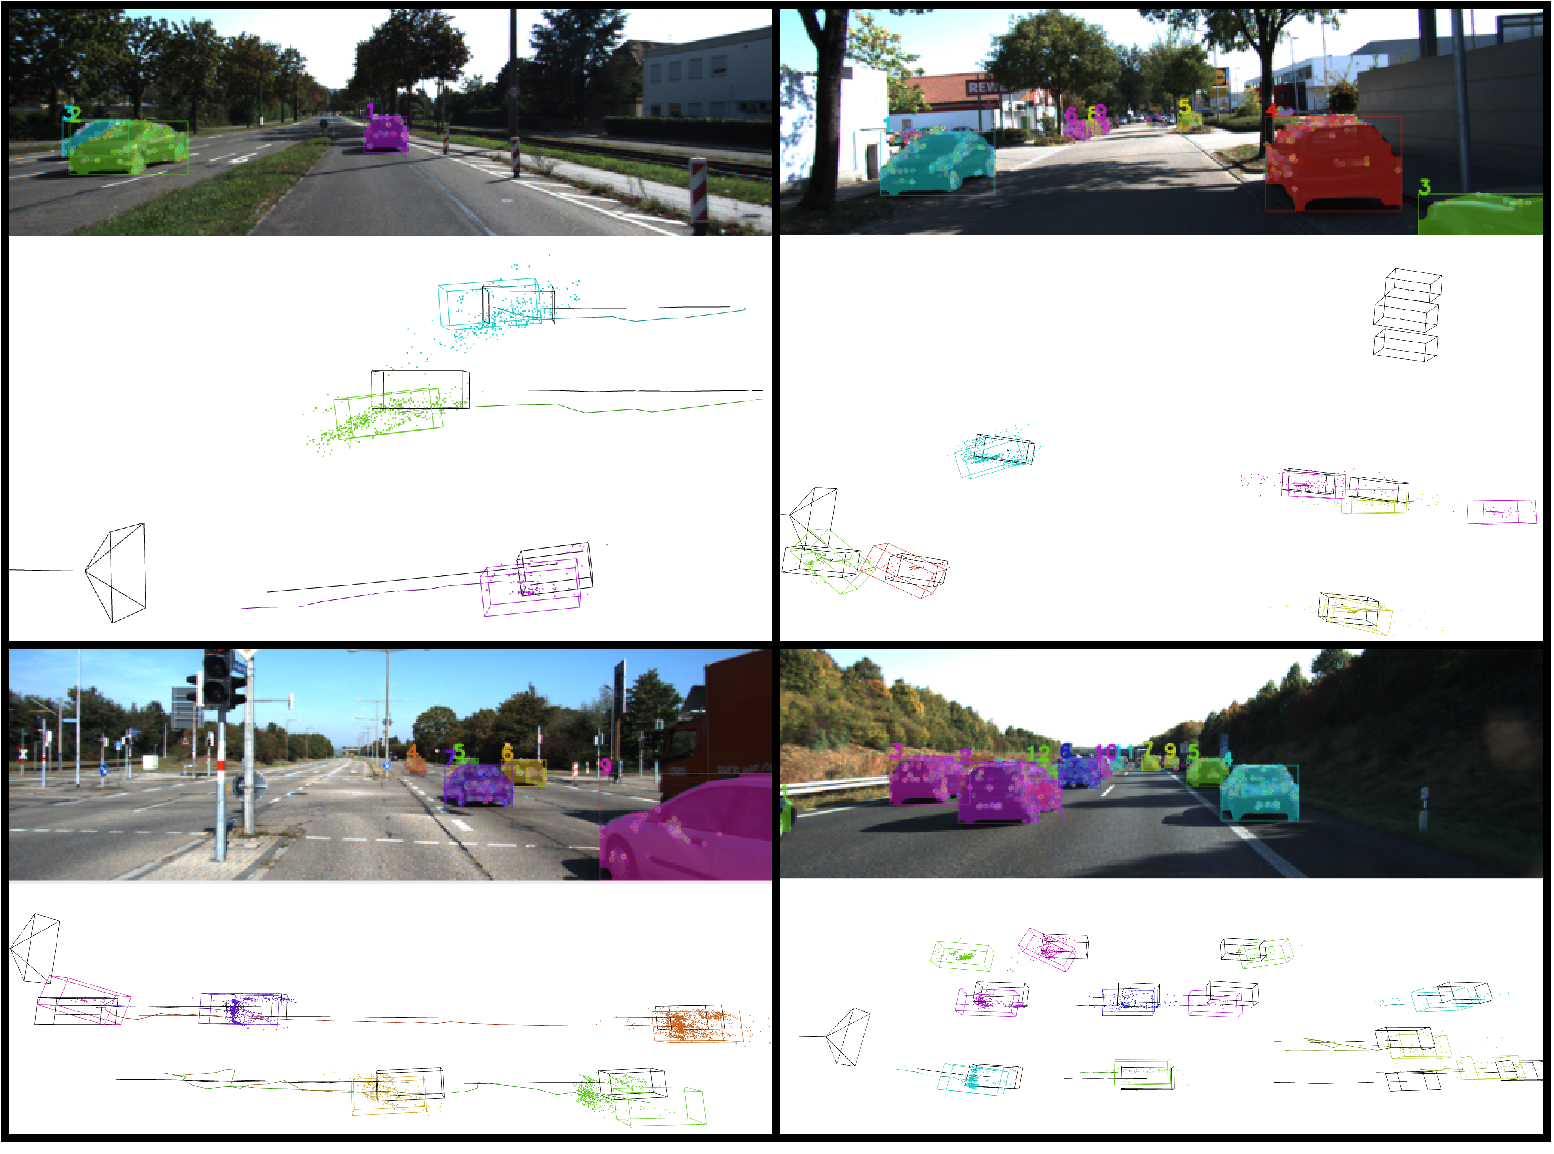
\includegraphics[width=\textwidth]{figures/more-scenes.pdf}
\caption{\label{fig:more-scenes}Several examples of BAMOT's ability to track cars. Each example consists of the RGB image and 2D detections above the 3D visualization of object tracks. Ground truth objects are in black; estimated tracks in color. \emph{Best viewed in color.}}
\end{figure}


As explained above, the sparsity of the proposed system and pedestrians' non-rigidity make it more difficult for \gls{bamot} to accurately track pedestrians compared to cars.
To track pedestrians well, enough of their nearly-rigid torso must be visible across frames to precisely localize and associate them. 
Compared to cars, single frame localization is also less precise since \gls{bamot} creates fewer landmarks on smaller objects. 
\cref{fig:pedestrians-good} shows some examples where the system is capable of localizing and tracking pedestrians. 
\cref{fig:pedestrians-bad} displays weak tracking ability scenarios: pedestrians are either localized imprecisely or lost and created as new tracks.


\begin{figure}[htbp]
\centering
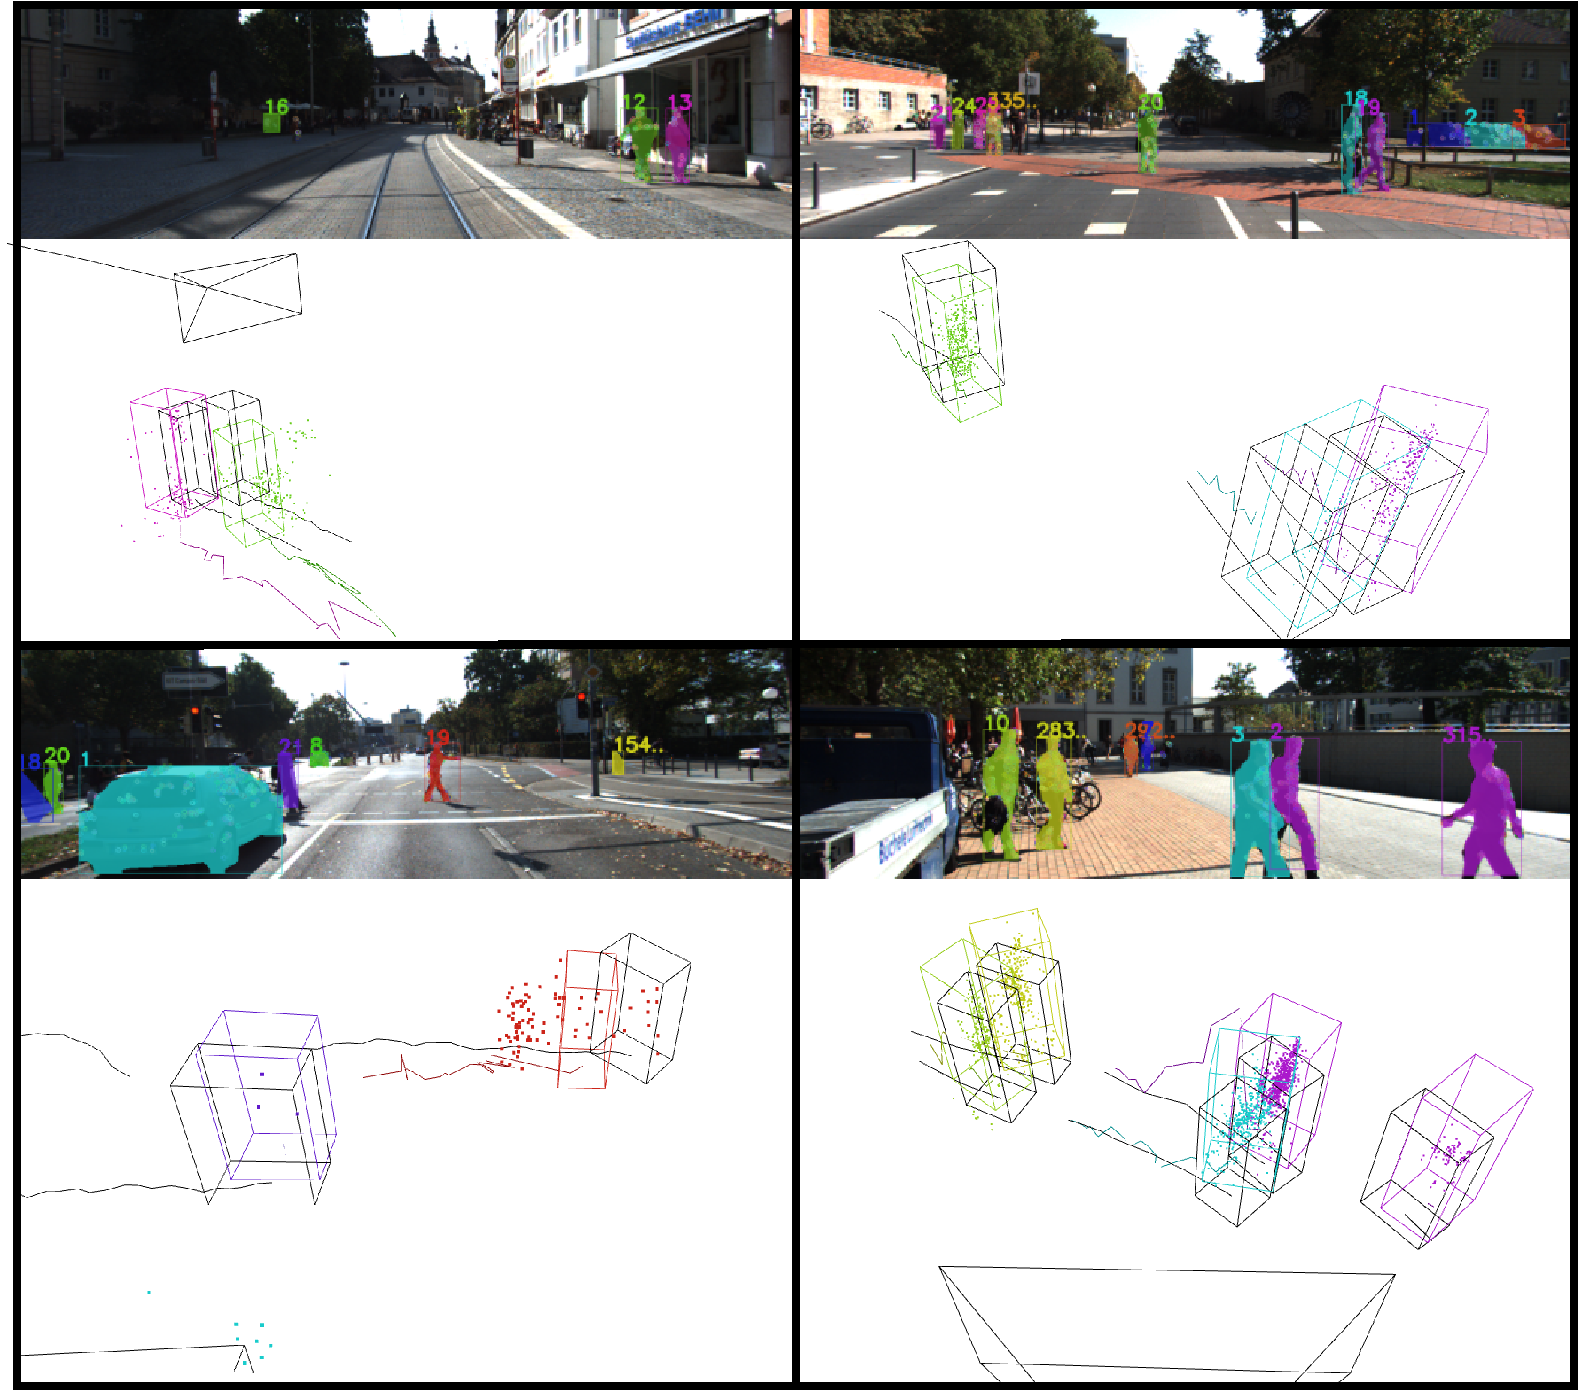
\includegraphics[width=\textwidth]{figures/peds-good.pdf}
\caption{\label{fig:pedestrians-good}When pedestrians are not occluded, \gls{bamot} can create enough landmarks to localize them accurately. Additionally, if they remain unoccluded for several frames, the system can track landmarks on their torso over time. \emph{Best viewed in color}.}
\end{figure}

\begin{figure}[htbp]
\centering
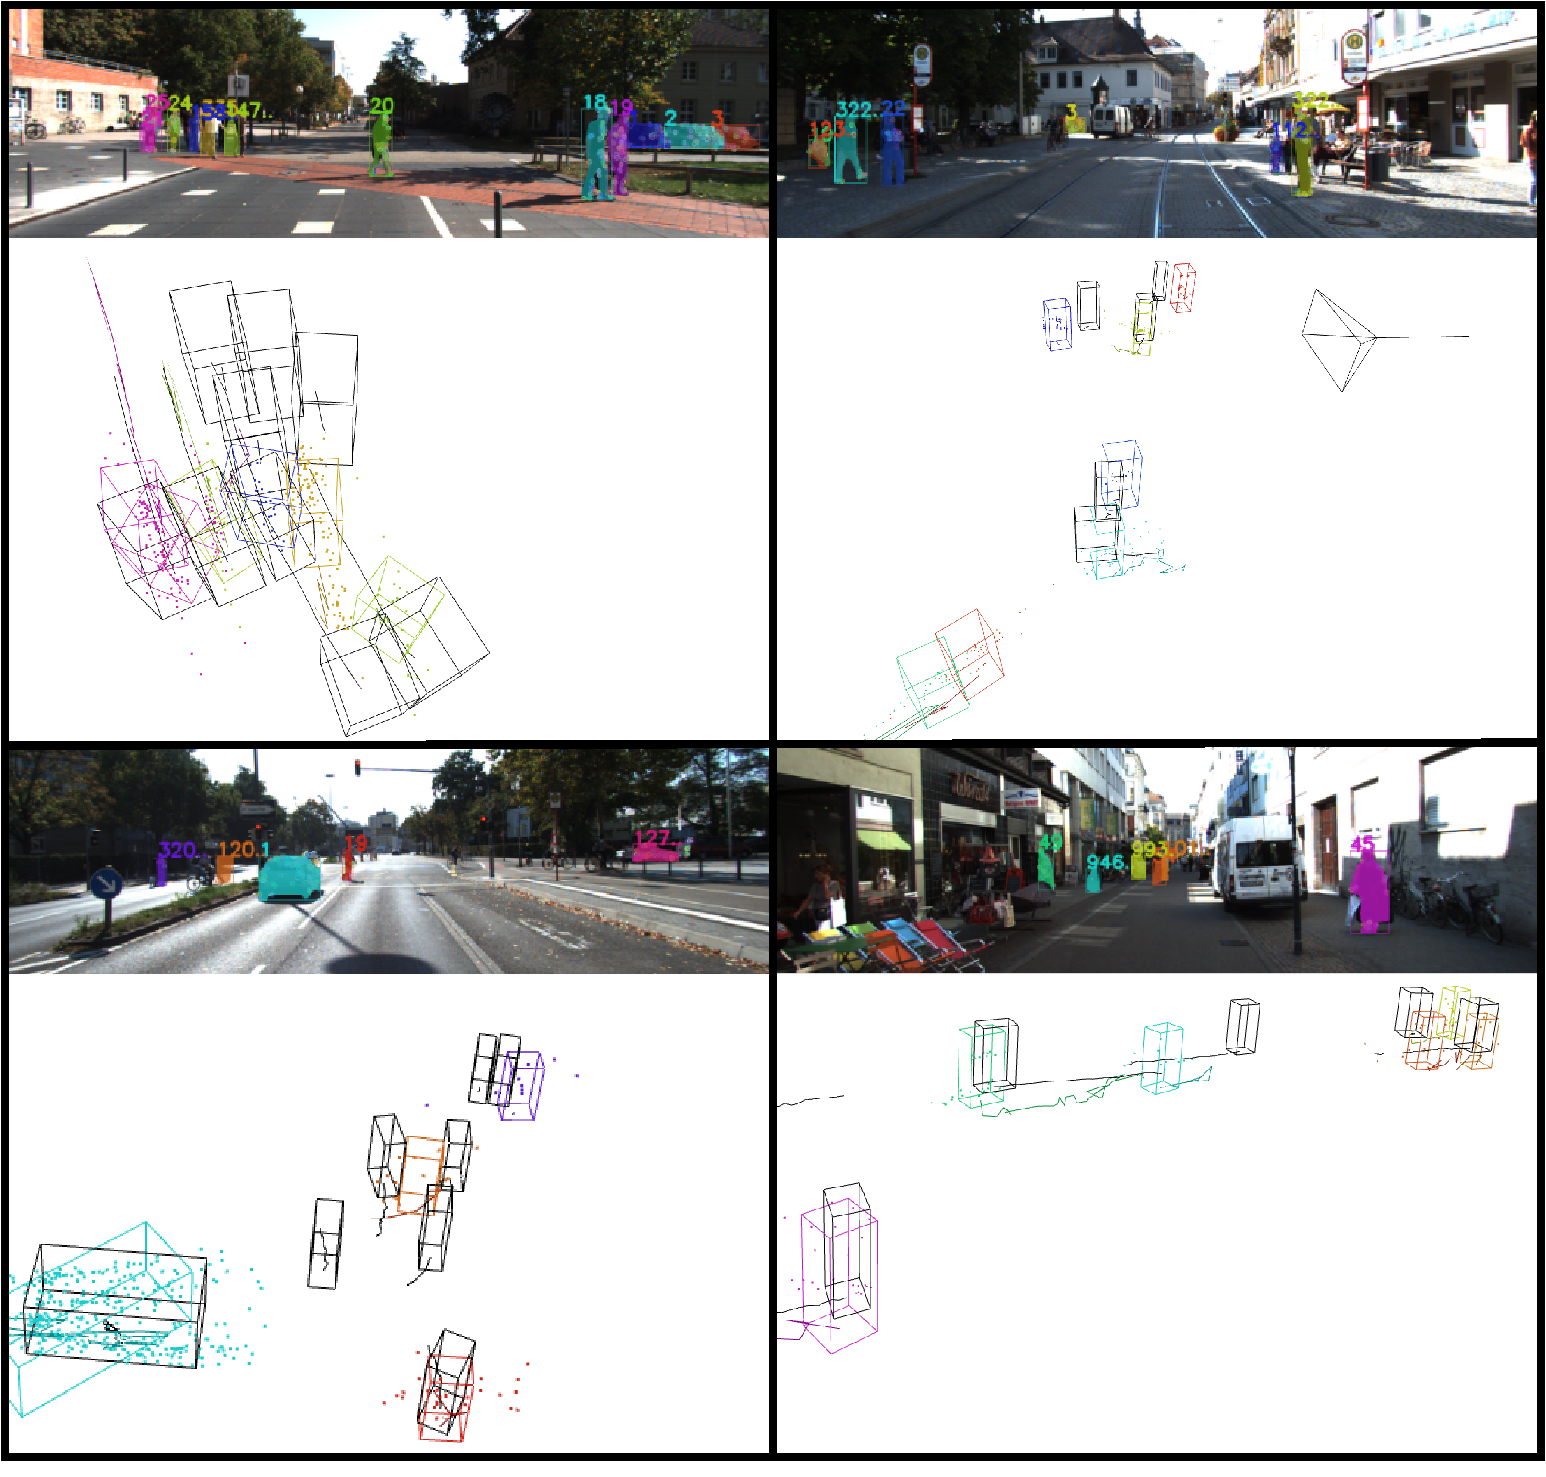
\includegraphics[width=\textwidth]{figures/peds-bad.pdf}
\caption{\label{fig:pedestrians-bad}The non-rigidity of pedestrians combined with our sparse approach makes association difficult. Often, pedestrian tracks are also not initialized because they are heavily occluded, and hence, our proposal cannot match enough features between the left and right image. This figure illustrates some difficult examples. \emph{Best viewed in color}.}
\end{figure}

The combination of appearance and 3D information for associating existing tracks to stereo detections improves association in several situations compared to the appearance-only procedure from TrackR-CNN.
One such example is shown in \cref{fig:improved-tracking}.

\begin{figure}[htbp]
\centering
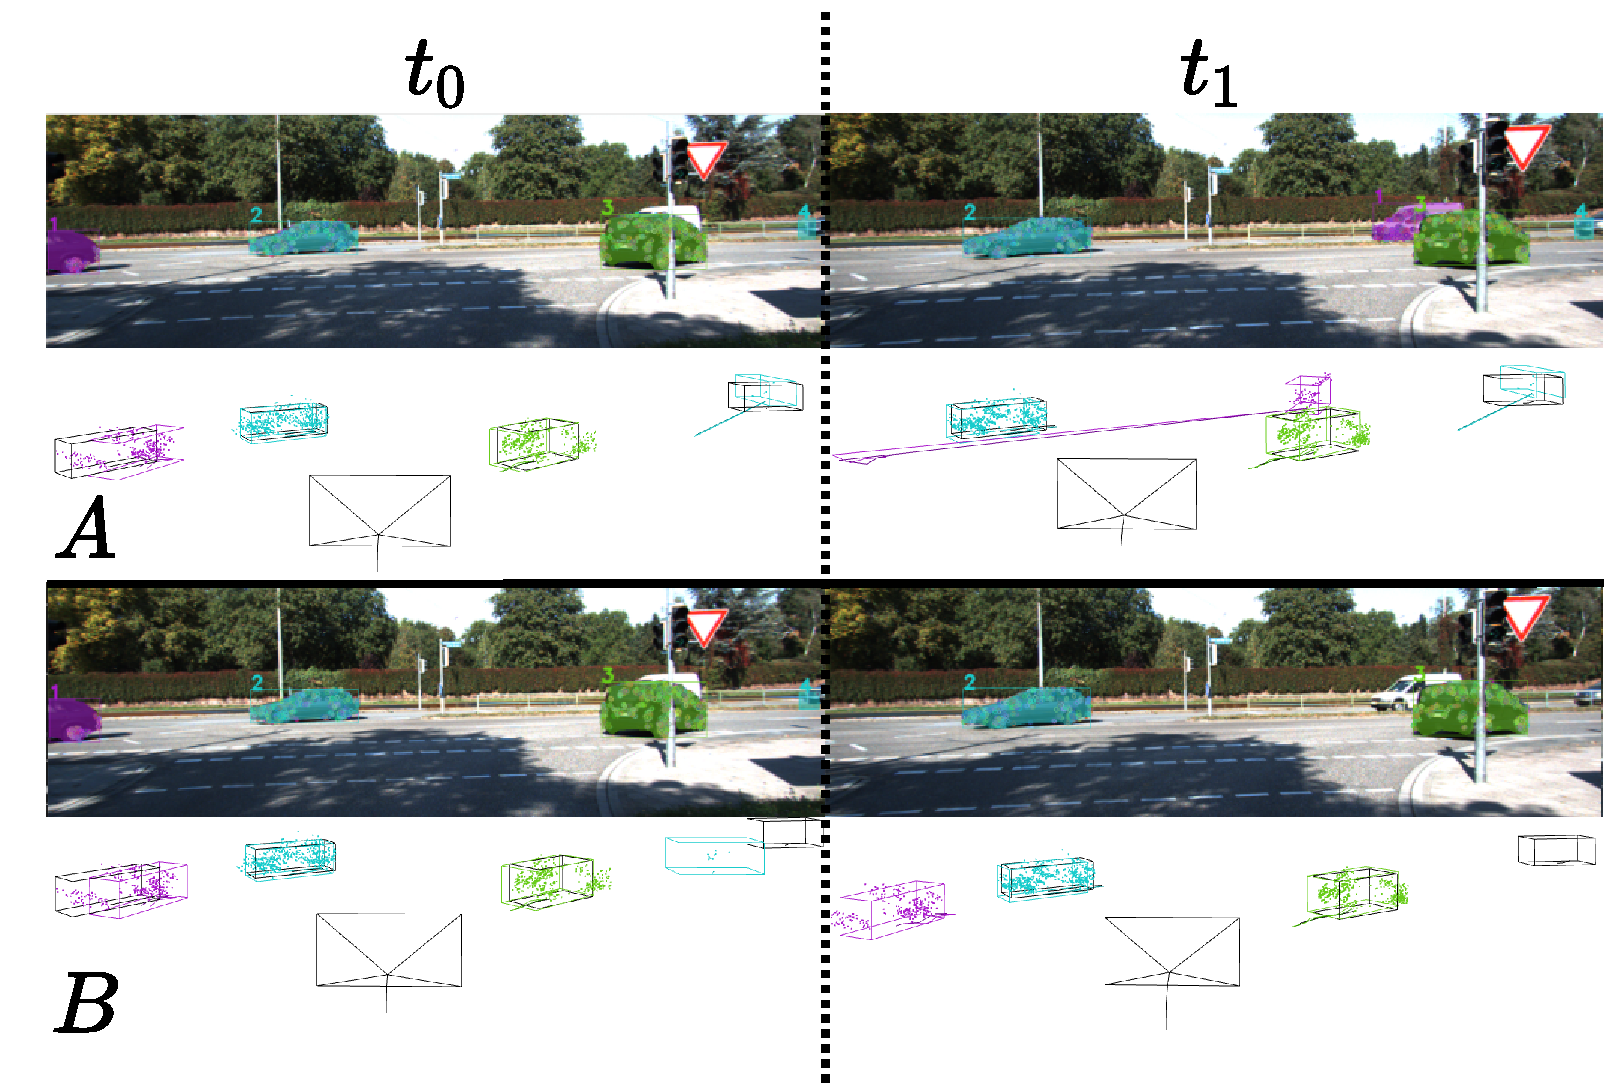
\includegraphics[width=\textwidth]{figures/improved-tracking.pdf}
\caption{\label{fig:improved-tracking}\emph{Top (A)}: Associations by TrackR-CNN are only appearance-based. Hence, associations between two frames \(t_0\) and \(t_1\) that make no sense in 3D are possible (far-left, purple bounding box). \emph{Bottom (B)}: Our association pipeline does take 3D information into account and, hence, the erroneous association from TrackR-CNN does not occur. Also, note the motion (and absence thereof) of the far-left (blue) bounding box: our system filtered a second incorrect association from TrackR-CNN in previous frames. \emph{Best viewed in color}.}
\end{figure}

Despite the discussed problems, \gls{bamot} works well in many cases, especially when considering localization only (i.e., object trajectories vs. \gls{oobb}). 
\cref{fig:trajs-10} and \cref{fig:trajs-4} illustrate such cases of accurately estimated trajectories. 
They also depict difficult situations such as parked cars or scenarios where IDSWs can occur.
\cref{fig:trajs-6} showcases how localization accuracy decreases with distance from the camera. The Figure, however, also shows how this is less of an issue if the track
is first localized close to the camera and then moves away from it.
Localization accuracy further declines when the landmark count decreases. 
For the trajectory figures, we match estimated trajectories to ground truth trajectories based on the average distance between detections weighted by the number of frames that tracks overlap.

\begin{figure}[htbp]
\centering
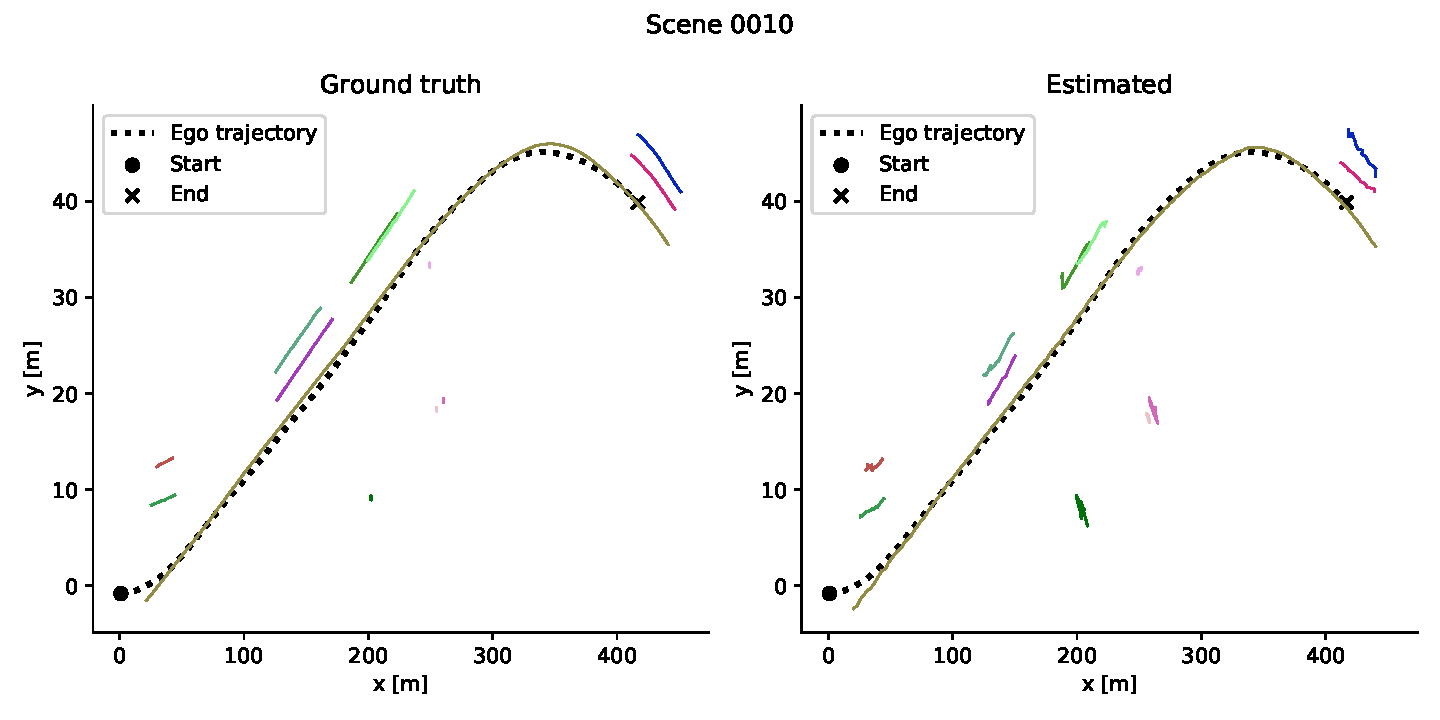
\includegraphics[width=.9\linewidth]{figures/trajs_10.pdf}
\caption{\label{fig:trajs-10}Our system performs well for moving cars as exemplified by these trajectories. However, parked cars at a distance often lead to jagged trajectories rather than points. One can also see how estimates become more accurate (and trajectories smoother) as we track the object for a longer period of time. \emph{Best viewed in color.}}
\end{figure}

\begin{figure}[htbp]
\centering
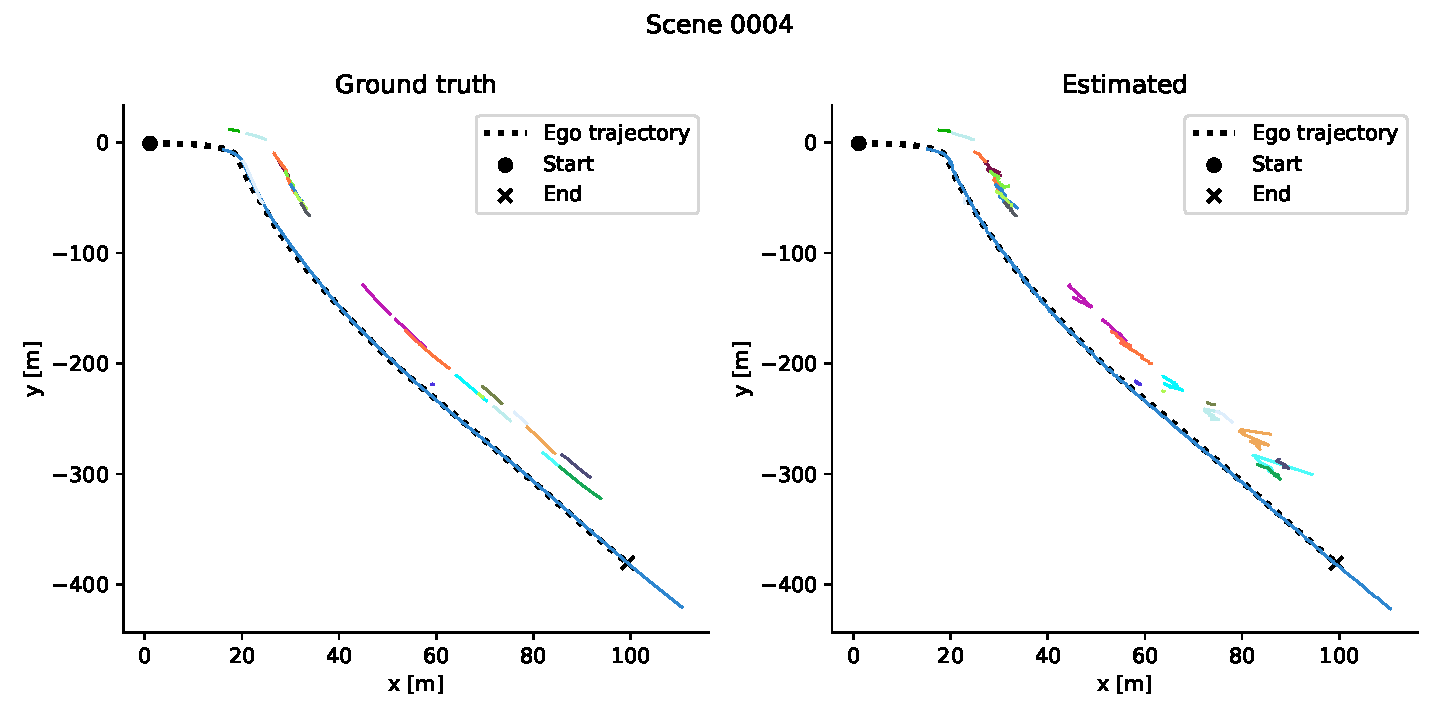
\includegraphics[width=.9\linewidth]{figures/trajs_4.pdf}
\caption{\label{fig:trajs-4}When an object is not tracked for several frames and far from the camera, our system allows for larger 3D motions. Generally, this improves performance. However, in some cases this can lead to IDSWs as exemplified by some of the inconsistent trajectories. \emph{Best viewed in color.}}
\end{figure}

\begin{figure}[htbp]
\centering
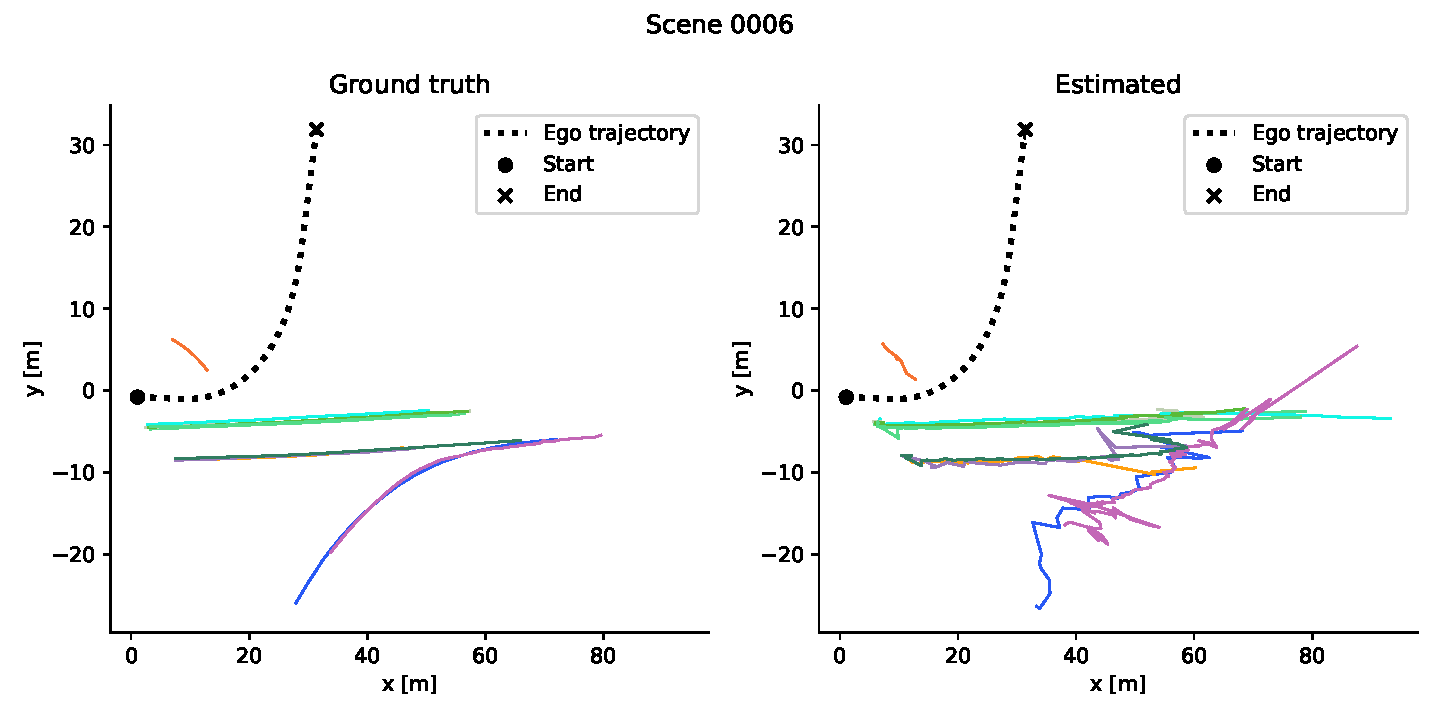
\includegraphics[width=\textwidth]{figures/trajs_6.pdf}
\caption{\label{fig:trajs-6}For most of the time, the ego-vehicle is at the left of this plot. This figure shows how the distance of objects w.r.t. the camera affects localization accuracy. Notice that the system can track trajectories longer than KITTI expects them to. However, in this scenario this does not count negatively towards the evaluation as both \gls{hota} and CLEAR ignore objects that are smaller than 25 pixels in the image domain. \emph{Best viewed in color.}}
\end{figure}



\chapter{Conclusion \& Future Work}
\label{sec:org32d6d7e}

\section{Conclusion}
\label{sec:org988f08c}
  In this thesis, we present a stereo-based approach for 3D \gls{mot}. 
Employing object-level \gls{ba} on sparse point clouds, a DL-based object detector, a novel hierarchical association pipeline that combines the objects' appearance and 3D information, and a priori assumptions about objects' shapes and dynamics,
we show encouraging results w.r.t. moving cars: object localization benefits from multi-frame tracking, as does orientation estimation leading to accurate \glspl{oobb}. 
Additionally, our association pipeline removes erroneous appearance-based associations by exploiting the available 3D knowledge our system keeps of objects.

We compare our system to the LiDAR-based AB3DMOT \cite{wengBaseline3DMultiObject2019} on the KITTI dataset \cite{geigerVisionMeetsRobotics2013}.
Since there exists no official 3D \gls{mot} benchmark for KITTI, and the adjustments presented in \cite{wengBaseline3DMultiObject2019} use the CLEAR \cite{bernardinEvaluatingMultipleObject2008} metrics with the flawed similarity measure of 3D \gls{iou},
we evaluate using a normalized 3D \gls{giou} on the recently introduced \gls{hota} \cite{luitenHOTAHigherOrder2021} metrics. We also present the corresponding CLEAR results.

While \cite{wengBaseline3DMultiObject2019} can more accurately localize objects due to the superior depth estimates of \glspl{lidar} vs. stereo-cameras, we show a possible comparative advantage when it comes to tracking.
Furthermore, we explore the impact of various implementation aspects of \gls{bamot}.
Due to our sparse approach and pedestrians' non-rigidity, \gls{bamot} demonstrates its capability to a greater degree for larger, rigid objects, namely cars.
The system's ability is most profound when the cars are moving (vs. parked) and initialized at not too-great distances (below \textasciitilde{}20 times the stereo baseline).

\section{Future Work}
\label{sec:org16677d7}
   Several approaches are possible to improve performance further.
First, orientation estimates for slow objects or those that haven't been detected in sufficiently many frames to estimate velocity accurately should be revised. 
Applying \gls{pca} to determine the dominant landmark point cloud axes may achieve this improvement in the before-mentioned situations. Second, there exists considerable research on extracting \glspl{oobb} from point clouds, e.g., \cite{qiFrustumPointNets3D2018,shiPointRCNN3DObject2019a}.
While these approaches assume dense \gls{lidar} point clouds, their results hint at the possibility of successfully training a similar network on sparse-point clouds. 
Adding our current \gls{oobb} estimates as initial guesses from which the network regresses may prove invaluable.

Also, comparing our approach to a dense stereo-based system, e.g., an adjusted MOTSFusion \cite{luitenTrackReconstructReconstruct2020} that stores \glspl{oobb}, should be insightful.
Ultimately,  KITTI adding a 3D \gls{mot} benchmark will allow us to compare against a wide variety of proposals. 

As discussed in \cref{related-work}, static \gls{slam} systems benefit from removing dynamic parts of the sensor input, so integrating our work with an existing visual \gls{slam} implementation is another possible direction of work.
For such integration to make the most sense, it is necessary to make \gls{bamot} real-time capable first.
This can be accomplished by performing object tracking in separate threads or processes and implementing \gls{bamot} in a compiled language.


\chapter{Appendix}
\label{sec:org975fd3e}
\begin{sidewaystable}[hb]
\centering
\footnotesize
\begin{tabular}{llrl}
Variable name & Description & Value & SI Unit\\
\hline
\(h^{ped}\) & fixed height of pedestrians & 1.9 & m\\
\(w^{ped}\) & fixed width of pedestrians & 0.7 & m\\
\(l^{ped}\) & fixed length of pedestrians & 0.9 & m\\
\(h^{car}\) & fixed height of cars & 1.6 & m\\
\(w^{car}\) & fixed width of cars & 1.8 & m\\
\(l^{car}\) & fixed length of cars & 4.3 & m\\
\(k^{car}_{min}\) & min. number of landmarks required to initialize track (car) & 13 & -\\
\(k^{ped}_{min}\) & min. number of landmarks required to initialize track (ped) & 3 & -\\
\(c_t^{car}\) & const. motion weight for translation in Bundle Adjustment (car) & 0.0015 & -\\
\(c_R^{car}\) & const. motion weight for rotation in Bundle Adjustment (car) & 50 & -\\
\(c_t^{ped}\) & const. motion weight for translation in Bundle Adjustment (ped) & 0.0005 & -\\
\(c_R^{ped}\) & const. motion weight for rotation in Bundle Adjustment (ped) & 0.005 & -\\
\(v_{max}^{car}\) & max. expected velocity (car) & 40 & m/s\\
\(v_{max}^{ped}\) & max. expected velocity (ped) & 8 & m/s\\
\(t_{bad}\) & max. number of consecutive frames w/ no detection before track is deleted & 11 & -\\
\(d_{max}^{c}\) & max. distance to current camera frame for newly triangulated landmark & 55 & m\\
\(n_w\) & sliding window size for Bundle Adjustment & 15 & -\\
\(n_v\) & sliding window size for calculating velocity vector & 10 & -\\
\(n_{rel}\) & sliding window size for calculating mean relative translation & 10 & -\\
\(n_{max}\) & size of uniform sample for computing landmark descriptor & 50 & -\\
\(f_{max}\) & constant in max. dist d\textsubscript{max} & 0.75 & -\\
\(\lambda_{pnp}\) & min. inlier ratio for PnP to be considered successful & 0.25 & -\\
\end{tabular}
\label{tab:hyperparameters}

\end{sidewaystable}

\microtypesetup{protrusion=false}
\listoffigures{}
\listoftables{}
\microtypesetup{protrusion=true}
\glsaddall
\printglossaries{}
\printbibliography{}
\end{document}
